% Preambel
\documentclass[a4paper,,openany,parskip=full]{scrreprt}
\usepackage[a4paper,left=3cm,right=3cm,top=3cm,bottom=3cm]{geometry}
%Sprache=deutsch, utf8 oder ansinew(Windows) für Umlaute
%code formatting
%Sourcecode Highlighting
%\usepackage{minted}
\usepackage{listings}
\usepackage[T1]{fontenc}
\usepackage[ngerman]{babel}
\usepackage[utf8]{inputenc}
%Schönschrift beim PDF erstellen
\usepackage{lmodern}
%Grafikunterstützung
\usepackage{graphicx}

%LandscapeGrafiken
\usepackage{wrapfig}
\usepackage{lscape}
\usepackage{rotating}
\usepackage{epstopdf}

%Farbliche Texte
\usepackage{xcolor}

%Zitate
\usepackage{csquotes}
%Farbige Hervorhebungen
\usepackage{soul}
\sethlcolor{blue}
%Tools
\usepackage{paralist}
\usepackage{enumitem}
\usepackage{caption}
\usepackage[section]{placeins}
\usepackage{float}

%Klickbare Links
\usepackage{hyperref}
\hypersetup{pdftitle={Pflichtenheft},
colorlinks=true, bookmarks, bookmarksnumbered}

\usepackage[nonumberlist, toc]{glossaries}
\makenoidxglossaries


% Versionierung
\newcommand{\version}{1.0}

\usepackage{color}
%Dokumentanfang


%% Json Formatting:
\colorlet{punct}{red!60!black}
\definecolor{background}{HTML}{EEEEEE}
\definecolor{delim}{RGB}{20,105,176}
\colorlet{numb}{magenta!60!black}

\lstdefinelanguage{json}{
    basicstyle=\normalfont\ttfamily,
    numbers=left,
    numberstyle=\scriptsize,
    stepnumber=1,
    numbersep=8pt,
    showstringspaces=false,
    breaklines=true,
    frame=lines,
    backgroundcolor=\color{background},
    literate=
     *{0}{{{\color{numb}0}}}{1}
      {1}{{{\color{numb}1}}}{1}
      {2}{{{\color{numb}2}}}{1}
      {3}{{{\color{numb}3}}}{1}
      {4}{{{\color{numb}4}}}{1}
      {5}{{{\color{numb}5}}}{1}
      {6}{{{\color{numb}6}}}{1}
      {7}{{{\color{numb}7}}}{1}
      {8}{{{\color{numb}8}}}{1}
      {9}{{{\color{numb}9}}}{1}
      {:}{{{\color{punct}{:}}}}{1}
      {,}{{{\color{punct}{,}}}}{1}
      {\{}{{{\color{delim}{\{}}}}{1}
      {\}}{{{\color{delim}{\}}}}}{1}
      {[}{{{\color{delim}{[}}}}{1}
      {]}{{{\color{delim}{]}}}}{1},
}



\begin{document}
\title{
	\huge{Entwurfsdokumentation}
	}
\subtitle{
	\vspace{1cm}
	  \Large {PSEKochbuch}\\
		\LARGE{Exzellenzkoch}
	\vspace{2cm}
	}
\date{
	\vspace{3cm}
	Wintersemester 2019/2020, \today \\
	\vspace{1cm}
	\vspace{1cm}
	}
\author{
		Magnus Bühler
		\and Wolf H. Lauppe
		\and Pascal Maier
		\and Thomas Weidmann
		\and Lea Strauch
		}
\maketitle

% ---------------------------------------------------------- Revisions-Historie

\newpage
\begin{table}[b]
\centering
\begin{tabular}{|l|l|l|l|p{0.4\textwidth}|}\hline
	\textbf{Version}	&\textbf{Autor}	&\textbf{Datum}	&\textbf{Status}	&\textbf{Kommentar}
\\\hline	1.0		&PSE3		&22.12.2019		&Abgabe				&Pflichtenheft v1.0 mit Ergänzung der Admin-Rolle
\\\hline	1.1		&PSE3		&07.01.2020		&				&Formatierungen, Domain Entity richtig eingebunden. 
\\\hline				&			&			&			&
\\\hline
\end{tabular}
\caption{\label{tab:revision}Versionshistorie}
\end{table}


%Inhaltsverzeichnis
\newpage
\pagenumbering{roman}
\tableofcontents
\newpage
\pagenumbering{arabic}

%Input einzelner Kapitel
\chapter{Zielbestimmung}

Dieses Dokument bietet ein Bericht zur Qualitätssicherung des Projektes "`Exzellenzkoch"'. Wie bereits in vorigen Dokumenten wird sich an den drei Schichten der zugrundeliegenden Clean Architecture orientiert:
\begin{itemize}
	\item User Interface Layer
	\item Data Layer
	\item Domain Layer
\end{itemize}
Die dokumentierten Testfälle beinhalten alle im Pflichtenheft spezifizierten Testfälle, die zum derzeitigen Implementierungsstand umsetzbar sind. Es werden also alle Muss-, sowie implementierte Wunschkriterien getestet.

\section{Paketübersicht}
\subsection{Client}
Generell teilen sich die Testpakete in zwei Stränge auf: Unittests und andere Tests.
Unittests sind im Paket \textbf{de.psekochbuch.exzellenzkoch} unter "`test"' zu finden und andere Tests in \textbf{de.psekochbuch.exzellenzkoch} unter "`androidTest"'. 
Unter "`andere Tests"' zählen sowohl die Tests des UI Layers, sowie auch die Repository- und Lasttests.
Die Tests des User Interface Layers befinden sich im Paket \textbf{de.psekochbuch.exzellenzkoch.testcases}, sowie in \textbf{de.psekochbuch.exzellenzkoch.navigation}.
Die Tests des Data Layers teilen sich auf in Servertests und Tests der Interface Implementierungen.
Repositorytests befinden sich im Paket
\textbf{de.psekochbuch.exzellenzkoch.datalayer}.
Der Server wird in seinem eigenen Repo getestet.
Lastentests sind im Paket \textbf{de.psekochbuch.exzellenzkoch.lastentest} zu finden.
Das Domain Layer enthält lediglich die Domain Entities, sowie die Interfaces, welche nicht getestet werden.

\subsection{Server}
Servertests befinden sich im Paket \\
\textbf{package de.psekochbuch.exzellenzkoch} unter "`test.kotlin"'
\chapter{Architektur}

\section{Prämisse}
Im Aufbau des Projekts wird das Konzept der "`Clean Architecture"' umgesetzt \cite{CleanArchitecture} \cite{AndroidGuidelines}. Das bedeutet, dass eine klare Modularisierung besteht. Kernfunktionen und Geschäftslogik werden von der Benutzeroberfläche, sowie von den Datenquellen getrennt. Somit sind die einzelnen Komponenten der Architektur leicht austauschbar. 
Die Grafik \ref{cleanarch} zeigt dieses Prinzip. Die grundlegenden Strukturelemente des Projekts liegt in "`Entity"'. In "`Use Case"' ist die Funktionalität der Entities enthalten.  Im oberen Teil des äußeren Rings ist die direkte Benutzeroberfläche, in der Eingaben verarbeitet werden, sowie die Abstraktion "`Presenter"', welche Logik zum Verarbeiten der Nutzereingaben stellt, zu sehen. Im unteren Teil bietet"`Repository"' eine Schnittstelle zu den verschiedenen Datenquellen, welche - genau wie "`UI"' - reale Einrichtungen (z.B. Datenbanken und Webserver) darstellen.
Dabei ist zu beachten, dass sich Abhängigkeiten einer äußeren Schicht nur auf innere Schicht beziehen dürfen, was anhand der unausgefüllten Pfeile sichtbar ist. Innere Schichten dürfen also keinerlei Wissen von Aufbau und Funktionalität von höher liegenden Schichten haben. Der Kern "`Entity"' hat demnach keine Abhängigkeiten. Dies ist das Prinzip der {\em Dependency Inversion}.
Der Datenfluss fließt trotz der Abhängigkeits-Regel bidirektional durch alle Schichten hindurch, da z.B. Daten, die aus einer Datenquelle geladen werden, auch in der Oberfläche sichtbar gemacht und dort ggf. auch geändert werden. Dies ist durch gewisse Entwurfsentscheidungen möglich, auf die in späteren Kapiteln noch näher eingegangen wird.


%Bsp-Grafik CleanArchitecture
\begin{figure}[H]
\centering
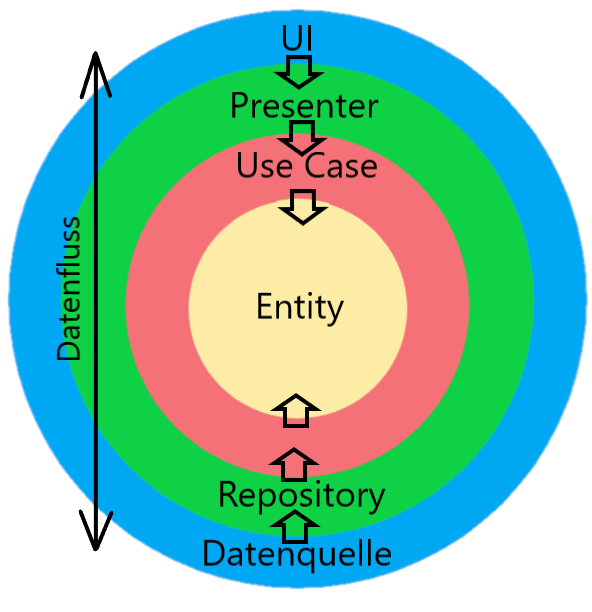
\includegraphics[width=0.51\textwidth]{pics/cleanArchitecture.png}%
\caption{Clean Architecture Prinzip grafisch dargestellt}%
\label{cleanarch}%
\end{figure}

\section{App}


\subsection{Layered Architecture}

Wenn man sich die konzentrischen Ringe von Robert C. Martins Clean Architecture einmal vertikal aufgeschnitten vorstellt, sieht man gut, dass die Clean Architecture zu einer Schichtenarchitektur führt, die den Code klar strukturiert.


\begin{itemize}
\item {\textbf{User Interface Layer}} (UI und Presenter)
\item {\textbf{Domain Layer}}  (Use Cases und Entities)
\item und {\textbf{Data Layer}}. (Repository, Datenquelle)
\end{itemize}


%Bsp-Grafik  Layer
\begin{figure}[H]
\centering
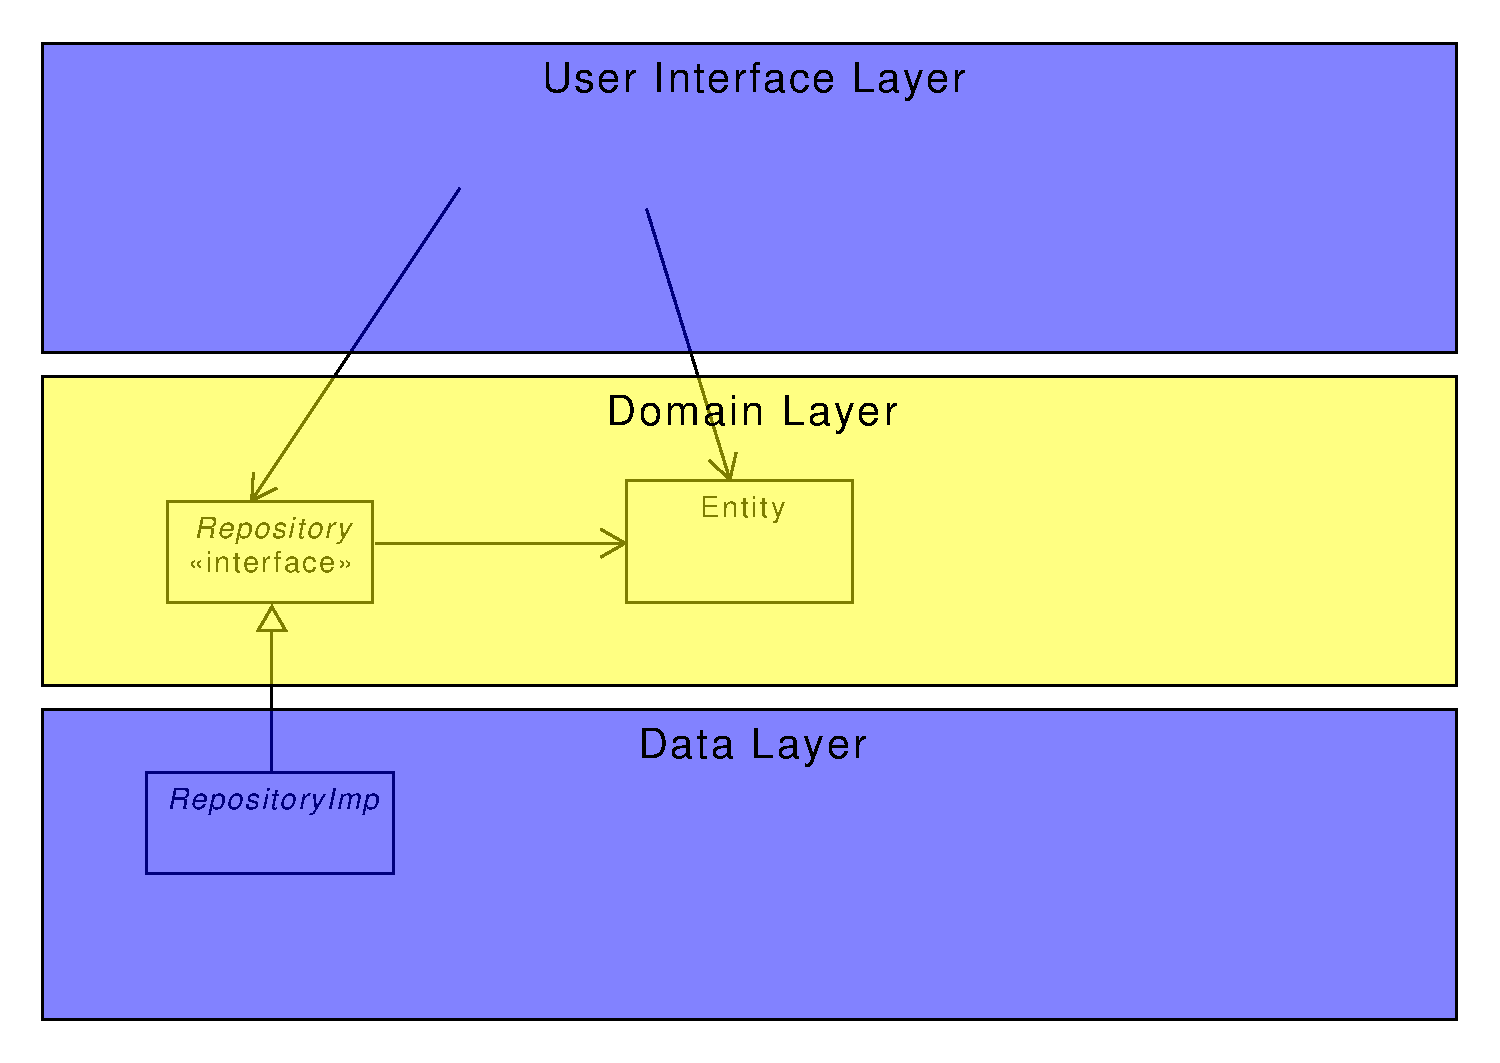
\includegraphics[width=0.5\textwidth]{pics/layers.pdf}%
\caption{Layer mit Dependency Inversion}%
\label{cleanarch}%
\end{figure}

\subsection{Domain Layer} 
Im Kern der Architektur steht die {\em Business Entities}, die unsere Domäne modellieren.
Diese beschreiben die "`realen"' Objekte unserer Domäne und die Methoden, die mit ihnen möglich sind. Genauer gesagt also Entitäten, wie zB. Rezepte, die es auch gäbe, wenn man das Kochbuch in Papierform führen würde. 

%Todo Glossarreferenz Clean Architekture Chapter 20 Business Rules

In diesem Entwurf ist das sogenannte "`Domain Driven Design"' umgesetzt \cite{CleanArchitecture} \cite{DomainDrivenDesign}, das heißt, dass die Kernentitäten szenariobasiert ermittelt wurden. Somit sind sie aus Szenariensicht von der Domäne aus und nicht von der Datenbank her modelliert.


\subsubsection{Repository-Schnittstelle}
Zusätzlich zu den Entitäten gehört zu dem innersten Kern der Clean Architecture die Repositoryschnittstelle für die einzelnen Entities.

Diese Schnittstelle kapselt, die durch die Datenzugriffsschicht persistierten Objekte und den Zugriff auf sie, unabhängig davon, ob sie lokal in der Datenbank gespeichert oder per Webservice zur Verfügung gestellt werden. 
Die Repository-Schnittstelle ist dabei als Schnittstelle (abstrakte Klasse) modelliert und stellt aus Sicht der Domain Logik, die nötigen Speicherfunktionen und Suchfunktionen, die die Anwendung braucht, dar. 

%Todo Referenz auf Repository Entwurfsmuster
%https://de.wikipedia.org/wiki/Repository_(Entwurfsmuster)
%Martin Fowler Patterns fo Enterprise Appplication 
%LI


\subsection{Data Layer} 
Die Datenschicht implementiert die Repositoryschnittstelle. Konzeptionell verhält sich das Repository aus Schnittstellensicht, wie eine Liste von Fachobjekten mit den bereitgestellten Methoden zum Laden und Speichern neuer Elemente.

In der Datenschicht wird zum einen die Persistierung in der lokalen SQLite Datenbank mit den in Android Bibliothek {\em Room} und zum anderen das Laden und Speichern der Objekte über die REST-Schnittstelle des Servers mit {\em Retrofit} umgesetzt. Die Bibliotheken sind von Google in den Android Jetpack Developer Guides empfohlen und werden deswegen eingebunden.

Jedes Repository wird mithilfe von DAOs (Data Access Objects) implementiert, die den Zugriff auf einzelne Tabellen in der Datenbank mit der relationalen Datenbanklogik zum Laden und Speichern kapseln. 

%\subsubsection{Dependency Inversion} 
%Was hier beschrieben ist, ist das Prinzip der {\em Dependency Inversion} 
%das Data Layer implementiert die abstrakten Repository Schnittstellen. 
%Dadurch wird genau die im Cleanarchitekturediagramm geforderte Abhängigkeit erreicht. Die Datenzugriffschicht hängt von dem Domain Layer ab
%und nicht umgekehrt. 

\subsection{UserInterface Layer}

\subsubsection{MVVM} 
Als Grundgerüst für die Strukturierung des User Interface Layer wird das Model-View-ViewModel (MVVM) Entwurfsmuster verwendet. 
Dabei beinhaltet "`View"' die grafische Benutzeroberfläche, sowie Anweisungen, wie auf Nutzer- und App Eingaben reagiert werden soll. 

Das "`ViewModel"' (VM) überwacht die View. Werden durch App-Interaktionen Daten in der View angefordert oder verändert, so merkt das VM dies und gibt dem Model die entsprechenden Befehle weiter. Es ist also ein Vermittler zwischen View und Model.
Durch die im Domain Layer beschriebenen Repositoryschnittstelle laden und speichern die ViewModellklassen Fachobjekte. 
%TODO Glossareintrag Fachobjekte

%Todo auf Fabrikmuster bezug nehmen. 
Das "`Model"' in MVVM steht für die Logik der grundlegenden App Funktionen. Im Falle von Exzellenzkoch sind das genau die Entityklassen und Repositoryschnittstellen, wie sie im Domain Layer definiert werden. 


\subsection{Zusammenfassung}
Ein Ziel dieser Architektur ist die Entkoppelung der sich ändern könnenden Schichten. So sind z.B. Nutzerschnittstelle und Datenschicht nur ein Detail. 

Die Anwendung wird so aufgebaut, dass zum Beispiel eine völlig andere Nutzerschnittstelle statt der Androidapp, oder ein dateibasierter Speicher statt einer relationalen Datenbank, umsetzbar wäre, ohne, dass dies auf die anderen Schichten Einfluss hätte.

Ein Vorteil, der dadurch entsteht, ist die klare Abgrenzung der einzelnen Funktionen und die leichtere Testbarkeit und Wartbarkeit der einzelnen Subsysteme. Außerdem wird durch diese Modularisierung das ganze Projekt leicht erweiterbar gemacht.

\section{Server}

\subsection{Einleitung}
Registriert sich ein Nutzer in der App, so kann er mit anderen Nutzer interagieren. Diese Interaktion wird durch die Serverkomponente ermöglicht. Ein eingeloggter User, kann mit der App auf seinem Smartphone Daten zum Server schicken und damit zum Beispiel Rezepte veröffentlichen. Andere eingeloggte User können dann nach diesen Rezepten suchen. 
Um dies zu ermöglichen, bietet der Server eine REST-Schnittstelle an. 
Unter verschiedenen "`Endpoints"' werden, ähnlich wie bei der Repositoryschnittstelle, verschiedene Methoden angeboten, um Entities zu laden und zu speichern. 

\subsubsection{Beispiel}
Ein HTTP GET auf den Endpunkt:

http://psekochbuch.de/api/users/MagnumMandel\footnote{Dies ist nur ein grober Überblick, modulo Authentifizierung. Ist diese aktiviert, erfolgt die Verbindung TLS-verschlüsselt. Gegebenenfalls leitet der Resource Server (unser Server) einen nicht authorisierten User an den Authentication Server von Google weiter, und erst wenn dieser mit korrektem JSON-Access-Token anfragt wird das JSON-Dokument als Antwort geschickt}


liefert zum Beispiel das passende JSON-Dokument zurück:
\begin{lstlisting}
{
  "userid": "MagnumMandel",
  ...
  "description": "Veganer essen meinem Essen das Essen weg."
}

\end{lstlisting}


Im Folgenden wird der Server mit seinen Komponenten näher beschrieben. 

\subsection{Technologiestack}
Der Server wird als Spring-Boot-Anwendung mit Rest-Schnittstelle umgesetzt.
Authentifizierung erfolgt nach dem OAuth 2.0 Standard mit JSON-Webtokens und soll mit Hilfe der Firebase Library verwirklicht werden. Die Daten werden mit Hilfe von Hibernate auf eine relationale Datenbank gemappt und gespeichert und geladen. 

\subsection{Struktur} 
Spring-Boot hat mit integrierter Dependency-injection und Annotationen einen klare Vorgabe, wie eine REST-Applikation umzusetzen ist. Mit verschiedenen Annotationen werden Klassen ausgezeichnet. Diese annotierten Klassen, die das Grundgerüst der Anwendung darstellen, werden Beans genannt. Der Spring IOC Container assembliert diese Beans dann, gemäß ihrer durch Annotationen bestimmten Rollen, zu einer Anwendung. 

\begin{figure}[H]
\centering
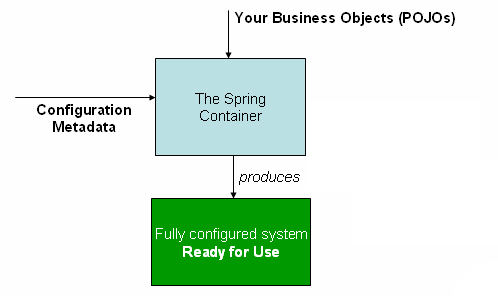
\includegraphics[width=0.6\textwidth]{pics/spring_ioc_container.png}%
\caption{Spring Inversion of Control Container\cite{SpringCoreTechnologies}}%
\label{cleanarch}%
\end{figure}

Der Server ist in verschiedene Bereiche aufgeteilt: \\
Zum einen gibt es eine Klasse, die die Einstellungen für den Server und die Logik für die Authentifizierung,  wie z.B. die Verbindung zu einer Authentifizierungsschnittstelle wie Firebase und die Überprüfung des JSON-Tokens,  beinhaltet. \\
Des weiteren gibt der Server eine API an, durch welche die Restschnittstelle mit ihren Endpunkten definiert wird. \\
Ein weiterer Bereich enthält die Logik für die Datenhaltung und Ansteuerung dieser API. \\

Die Paketeinteilung ist in Kapitel 4.2 erläutert. 
\section{Deployment}
 
\subsection{Server-Deployment} 
Als Springboot-Applikation ist die deploybare App des Servers ein JAR-File, dass den HTTP-Server Tomcat und alle Abhängigkeiten enthält. Es braucht kein vollwertigen Java EE Server konfiguriert und installiert werden, der dann einem WAR oder EAR bestückt. Das heißt als Umgebung auf unserem Bw-Cloud-server wird nur ein Linuxsystem mit installiertem JavaJDK und eine relationale Datenbank benötigt. 

\subsection{App-Deployment}
Das Gradle Build-tool erstellt eine apk-Datei, die alle benötigten Bibliotheken, die nicht auf den Endgeräten vorausgesetzt werden und das Manifest, was die Installation spezifiziert, enthält. Die apk-Datei kann dann entweder über das Android Debug Bridge-Tool (adb) direkt auf ein Endgerät installiert oder über den {\em Google Play Marketplace} veröffentlicht werden.


\section{Authentifizierung und Authorisierung} 
Die App und der Server sollen ein Rechtemodell umsetzen. 
Das bedeutet, dass Nutzer, je nach Status, unterschiedliche Rechte für die Nutzung der Funktionalität der App, besitzen. Beispielsweise soll jeder Nutzer, auch wenn er noch keinen Account hat, nach Rezepten suchen können. Das Updaten und Löschen eines öffentlichen Rezeptes (also das "`Neuveröffentlichen"') soll nur dem jeweiligen Autor gestattet sein. Kommentare zu Rezepten posten können nur eingeloggte Nutzer mit Account.
Ein Nutzer, der den Status "`Admin"' hat, kann in der Rolle des Admin auch Rezepte fremder Nutzer löschen. 

Das bedeutet, dass es eine Authentifizierung und eine Authentisierung von Nutzern im Server geben muss. Diese soll dem OAuth 2.0 Standard mit JSON-Webtokens genügen.

Bei OAuth 2.0 wird das Passwort nur beim Log-In verschickt. Als Antwort bekommt der Client zwei Token zurück.
Weitere Anfragen werden nur mithilfe des ersten Tokens durchgeführt. 
Dieses Token {\em access token genannt} ersetzt das Passwort für eine bestimmte Zeit. 
Ist die Zeit abgelaufen, kann der Client mit dem zweiten Token, dem {\em refresh token} sich ein neues Token holen. 

Das Access Token ist nicht zufällig generiert, sondern enthält die ID des Users und Metainformationen, wie das Ablaufdatum des Tokens. Es ist mithilfe eines Schlüssels signiert, sodass es nicht gefälscht werden kann. 
Jeder Service kann somit sowohl den User, als auch die Metainformationen, aus dem JSON-Token abrufen, ohne sich diese Informationen merken zu müssen.

Um dies zu implementieren, werden die Funktionen der Google Firebase API angewendet. 
Diese besitzt, für die App-Komponente und für den Server, Libraries, die die meisten Teile des Protokolls transparent und standardisiert dem OpenID-Connect-Standard genügen. 
Das heißt, der Authorization-Server und damit auch die Passwort- und Accountverwaltung wird von Google gestellt, so wie es nach Abgrenzungskriterium A1 vorgegeben ist. 
Der eigens implementierte Server dieses Projekts, ist der Ressource-Server. 

\subsection{Adminrolle} 
Der oben beschriebene Aufbau von Oauth 2.0 und den JSON-Webtokens, erlaubt eine elegante Umsetzung der Adminrolle, durch Hinzufügen eines "`Custom Claims"'. Diesen kann der Operator des Servers über die Firebase-Konsole von Google für einzelne Accounts festlegen.

Dann ist dieser Custom Claim im Payload-Feld des JSON-Webtokens verfügbar und der Zugriff von den HTTP Endpoints auf die REST-Schnittstelle kann entsprechend beschränkt werden. 

Das JSON-Web-Token hat also beispielsweise ein Feld wie folgt:

\begin{lstlisting}
{
 "loggedInAs" : "admin",
}
\end{lstlisting}

Aufgrund dieses Feldes kann der Server, pro Zugriff auf eine spezielle Funktion, entscheiden, ob der Zugriff erlaubt wird oder nicht. 

\section{Entwurfsentscheidungen}
Der Server wird wie beschrieben mit Spring Boot umgesetzt. 
Es wurde entschieden  als Programmiersprache sowohl für den Server als auch für die App Kotlin zu verwenden.
Als Build-automatiserungs-Tool wird für Server und App Gradle verwendet. 

Inzwischen wird Kotlin und Gradle sowohl von Springboot als auch dem Androidframework mit einem gewissen Reifegrad unterstützt. Die Entscheidung dieselbe Sprache und dasselbe Buildsystem zu nehmen garantiert eine gewisse Vereinheitlichung der Tools in der Entwicklung. 
Kotlin als Sprache erlaubt eine objektorientierte Entwicklung, was eines der Ziele des PSE-Praktikums ist. 

Spring Boot, hat mit seinem "`convention-over-configuration"`-Ansatz sehr klare Architektur-und Konfigurationsempfehlungen, was einen Aufbau mit guter Struktur vereinfacht. 
 
Die Schnittstelle zwischen Server und App als REST-Schnittstelle mit DTOs zu definieren, ist ein gewisser Mehraufwand. Man könnte, da Server und App beide in Kotlin geschrieben sind, auch zum Beispiel RMI verwenden. Der Vorteil ist, dass mit der REST-Schnittstelle und den DTOs ein klarer Vertrag  zwischen Server und App und eine klare Trennung erzielt wird. Dies erleichtert das Testen der einzelnen Komponenten und das Bearbeiten der App und Server in Subteams mit reduziertem Kommunikationsaufwand. 

Auch ist REST inzwischen der vorherrschende Standard, um einen Webservice umzusetzen. Die Unterstützung ist gut in das Spring-Boot-Framework integriert. 

Rest ermöglicht HTTP Technologien wie Caching zu Verwenden. Das ist ein Konfigurationspunkt für LoadBalancing, der eine spätere Skalierung auf mehrere Server einfach möglich machen würde, wenn dies irgendwann benötigt werden würde.  

Der gewählte Ansatz mit  SpringBoot ermöglicht es die Serveranwendung als eine deploybare Datei auf einem eigenen Server zu installieren. Das reduziert den Deploymentaufwand im Gegensatz zu einem Deployment mit einem  eigenständigen Application Server beträchtlich. 

Installation auf einem selbst administrierten Linux-Server bedeutet, dass Javaumgebung und relationale Datenbank selbst administriert werden müssen. 

Eine  Alternative zu dieser Herangehensweise wäre eine der vielen Cloud Platformen zu wählen zum Beispiel Amazon Elastic Compute Cloud oder Google App Engine. Damit würden Schritte, wie das Aufsetzen einer Datenbank entfallen. 

Gleichzeitig würde dies den Server an eine vendorspezifische Auswahl von Programmiersprachen APIs und Frameworks binden. 
Dies wird mit dem gewählten Ansatz für den Server versucht zu verringern. 




\chapter{Interaktion zwischen Komponenten}

\section{Interaktion von App Komponenten}
 
\begin{figure}[H]
\centering
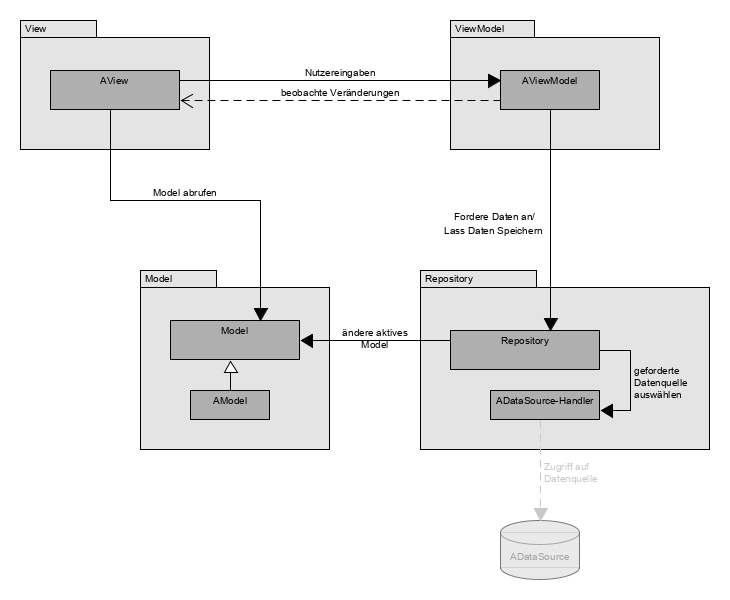
\includegraphics[width=0.7\textwidth]{pics/appComponentInteractions.png}%
\caption{Interaktion der App-Komponenten}%
\label{appcomp}%
\end{figure}


%AppComponentInteractions UML hier einfügen
Diagramm \ref{appcomp} beschreibt die Interaktion zwischen den einzelnen App-Komponenten etwas spezifischer als im vorigen Kapitel.
Zu beachten ist dabei, dass die angezeigten Komponenten "`AView"', "`AViewModel"', "`AModel"' und "`DataSource"' nur beispielhafte Instanzen darstellen. Jedes der ihnen zugrundeliegenden Pakete kann noch weitere Instanzen enthalten, die hier zur Anschaulichkeit vernachlässigt wurden.
Die Interaktion der App-Komponenten funktioniert folgendermaßen:
Ändert ein Nutzer Daten über die Benutzeroberfläche, so wird in der derzeit aktiven View-Komponente ("`AView"') eine Änderung vom zugehörigen ViewModel ("`AViewModel) registriert. Dieses gibt an das Repository durch, welche Daten geladen oder verändert werden müssen. Das Repository fordert daraufhin entweder Daten vom Server an, bzw. veranlasst eine Aktualisierung der Serverdaten, oder es holt, bzw. aktualisiert die Daten aus der lokalen SQLite-Datenbank ("`ADataSource"'). Außerdem aktualisiert das Repository das momentan aktive Model ("`AModel"') und gibt diesem die gerade geladenen oder aktualisierten Daten. Dadurch können neue Daten in der View angezeigt werden.

\section{Interaktion von Serverkomponenten}

In dem API Package des Servers(siehe Kapitel 4.2) befindet sich eine Menge an Interfaces, die angeben, wie man vom Client auf die API zugreifen kann. Diese Interfaces werden von den Controller-Klassen implementiert, insbesondere wird jede API-Klasse von einem zugehörigen Controller implementiert. 
Die Controller bearbeiten die Anfragen, die von den App-Klassen an den Server gestellt werden. Dabei rufen sie Serviceklassen auf, welche dann auf sogenannte "`Data Access Objekte"' (DAOs) zugreifen, um entweder Daten zu laden oder Daten zu speichern. Die Serviceklassen geben, wenn Daten angefragt wurden, die geladenen Daten an die Controller zurück und durch die Controller werden dann die Daten an den Client geschickt.
Bevor ein Client Daten anfragen oder senden kann, muss dieser erst Authentifiziert werden. Dazu wird ein JSON-Web-Authentification-Token, welcher bei der Anfrage mitgesendet wird, durch die Firebaselibrary überprüft.


\section{App- und Server-Kommunikation}

\begin{figure}[H]
\centering
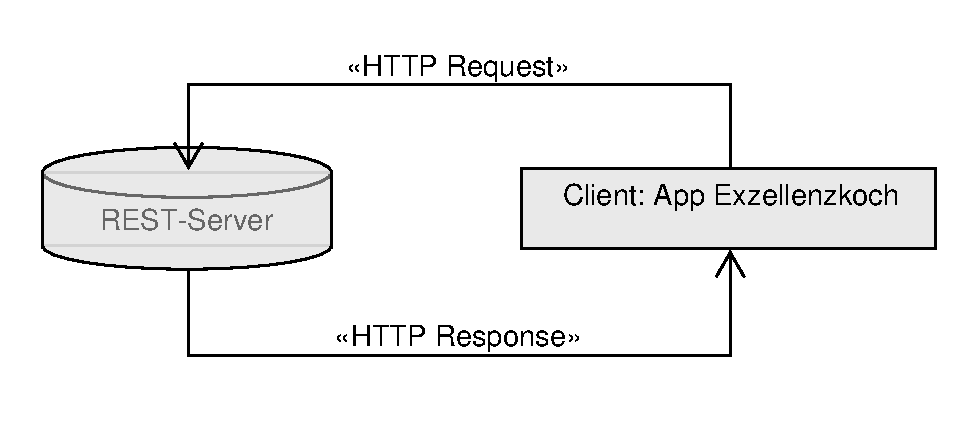
\includegraphics[width=0.7\textwidth]{pics/ServerAppRESTInteraction.pdf}%
\caption{Server-AppkKommunikation über REST}%
\label{rest}%
\end{figure}

Der Server bietet eine REST-Schnittstelle. Über diesen kommunizieren App und Server miteinander.
Hierbei wird das Request-Response Verfahren verwendet, wie in Abbildung \ref{rest} vereinfacht gezeigt. Der Client schickt eine Anfrage an den Server. Eine Anfrage verwendet das HTTP-Protokoll. Entweder wird eine GET-, POST-, PUT- oder DELETE-Anfrage gesendet. Der Server bearbeitet die Anfrage und gibt eine Antwort zurück. Die Daten werden als JSON-Dateien versendet. Die Verbindung zwischen Client und Server besteht, solange die Anfrage und Antwort durchgeführt, oder eine Zeitbegrenzung überschritten wird. 
Statt dass die App ganze Entity-Objekte an den Server sendet, werden diese in "`Data Transfer Objects"' (DTOs) abstrahiert. Die DTOs sind so aufgebaut, dass sie auf die Server-Datenbank Tabellen gemapped werden können. Mehr zum Aufbau der DTOs ist in Kapitel \ref{kapdtos} zu finden.
%https://www.itwissen.info/Request-Response-Verfahren-request-response-method.html

%\section{Interaktion der Appkomponenten} 
%Grafik \ref{rrr} zeigt ein einen Überblick über die Interaktion in MVVM mit eingebundenem Data Layer. Hier sieht man an einer möglichen Umsetzung der Architektur 
%\begin{figure}[!htbp]
%\centering
%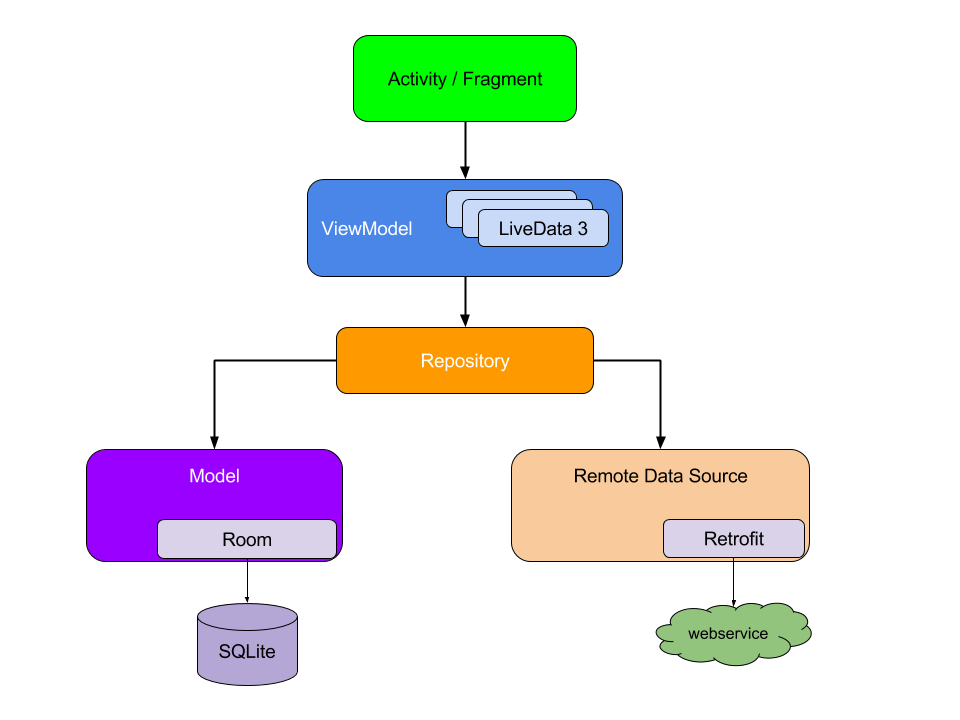
\includegraphics[width=0.7\textwidth]{pics/MVVM_repository.png}
%\caption{MVVM mit Data Layer  \cite{AndroidArchitectureComponents}}%
%\label{rrr}%
%\end{figure}
%die Aufteilung in View ("`Activity/Fragment"'), ViewModel, Model und Data Layer mit bestehendem Repository als Zugriffs-Abstraktion.

\chapter{Paketeinteilung und Klasseninteraktion}

\section{App}

\subsection{User Interface Layer} 

\subsection{View}

\begin{figure}[H]
	\centering
	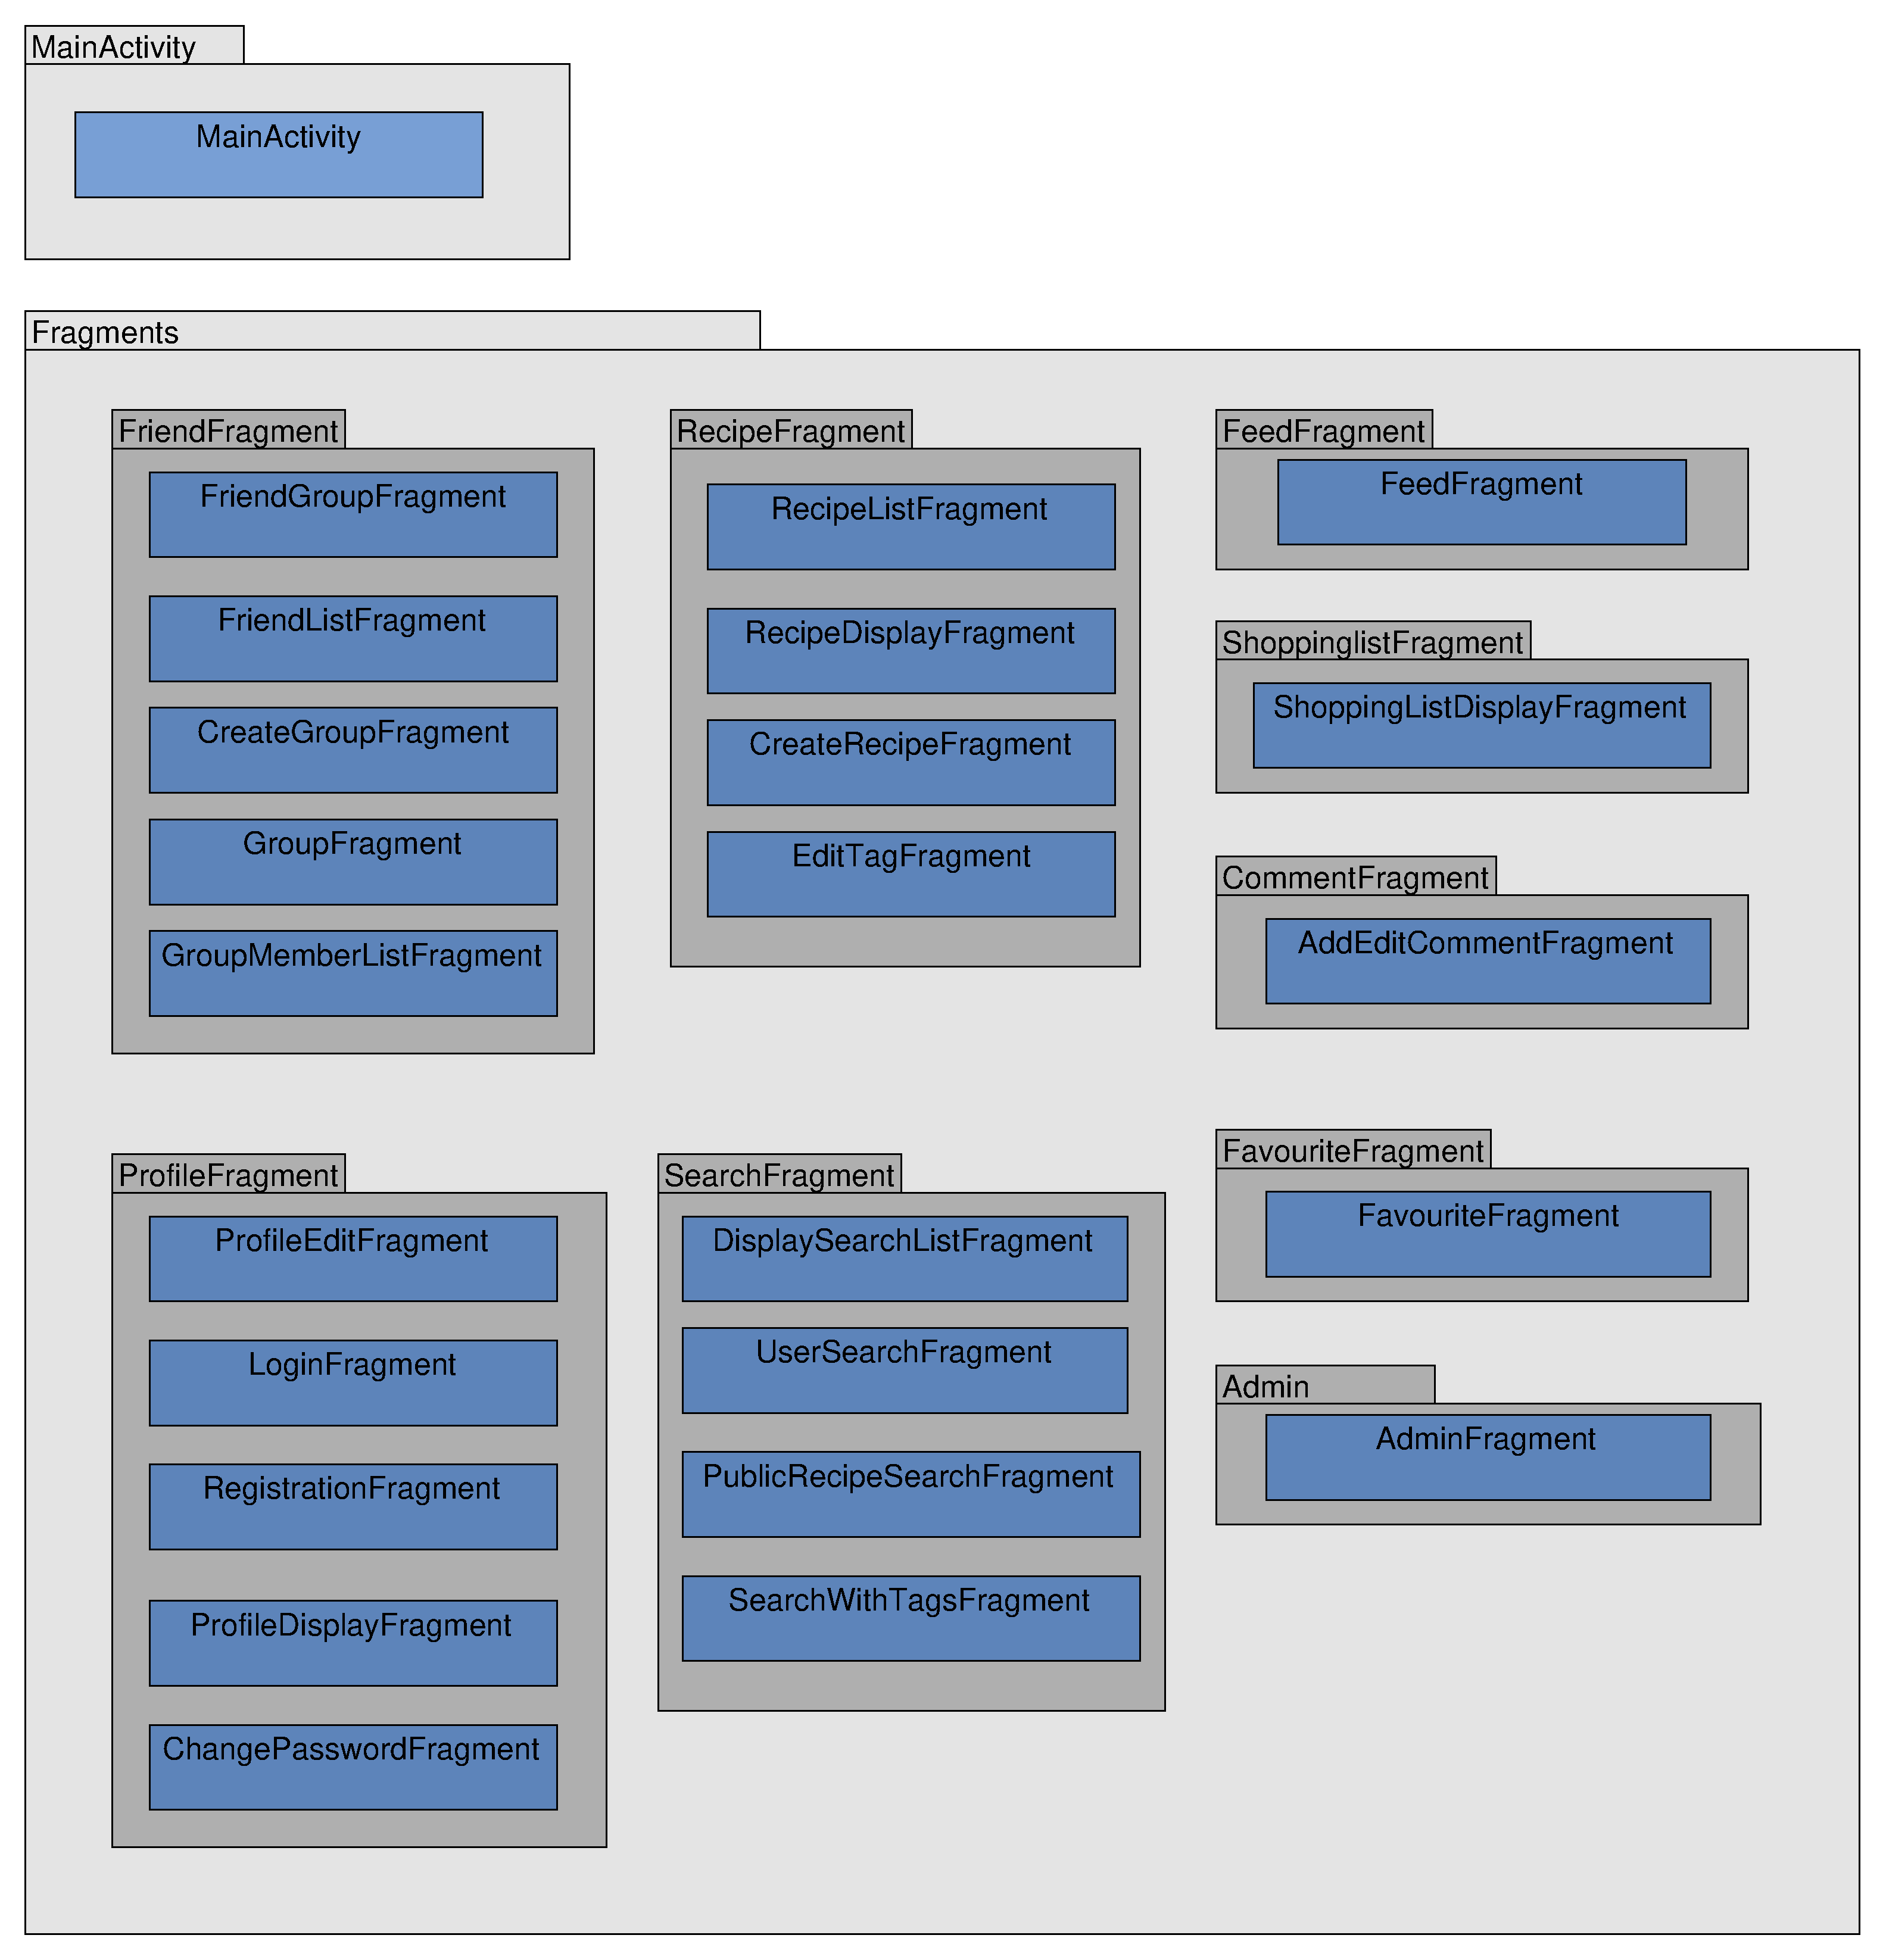
\includegraphics[width=1\textwidth]{pics/viewPackages/ViewPaketmodel.pdf}%
	\caption{Einzelne Pakete des User Interface Layers}%
	\label{view}%
\end{figure}

Die in Abbildung \ref{view} gezeigten Klassen sind die Klassen der View.
Die View erhält die Benutzereingabe direkt. Die grafische Oberfläche besteht aus einer Hauptaktivität, auch MainActivity, die durch ein Menü Fragments aufrufen kann. Das Menü ist ein eigenes Fragment, welches in der Toolbar der MainActivity zu sehen ist (mehr dazu in Kapitel 5.1). Die Fragments sind Klassen, denen .xml-Dateien zugeordnet sind und die die verschiedenen Oberflächen darstellen.

Abbildung \ref{viewinteract} zeigt einen groben Überblick über die Interaktion zwischen allen Fragments und der MainActivity. Die Pfeile zwischen den Fragments zeigen an, welche Fragments uni- oder bidirektionale Aufrufe aufeinander haben. Da das Menü in der Toolbar stets sichtbar ist, gibt es von jedem Fragment auch eine Interaktion "`Menü öffnen"', welche in \ref{viewinteract} im Sinne der Übersichtlichkeit nicht extra dargestellt wird. 
Was ebenfalls nur exemplarisch modelliert ist, ist der "`Zurück"'-Button des Smartphones, über den jedes Fragment verlassen werden kann. Nutzt man den "`Zurück"'-Button, gelangt man zurück auf das vorher angezeigte Fragment. Gibt es kein vorheriges Fragment mehr, weil man auf der Startseite der App ist, verlässt man die App mit dem Button.
Folgende Grafiken beschreiben nun genauer die Interaktionen zwischen den Fragments.

\begin{figure}[H]
	\centering
	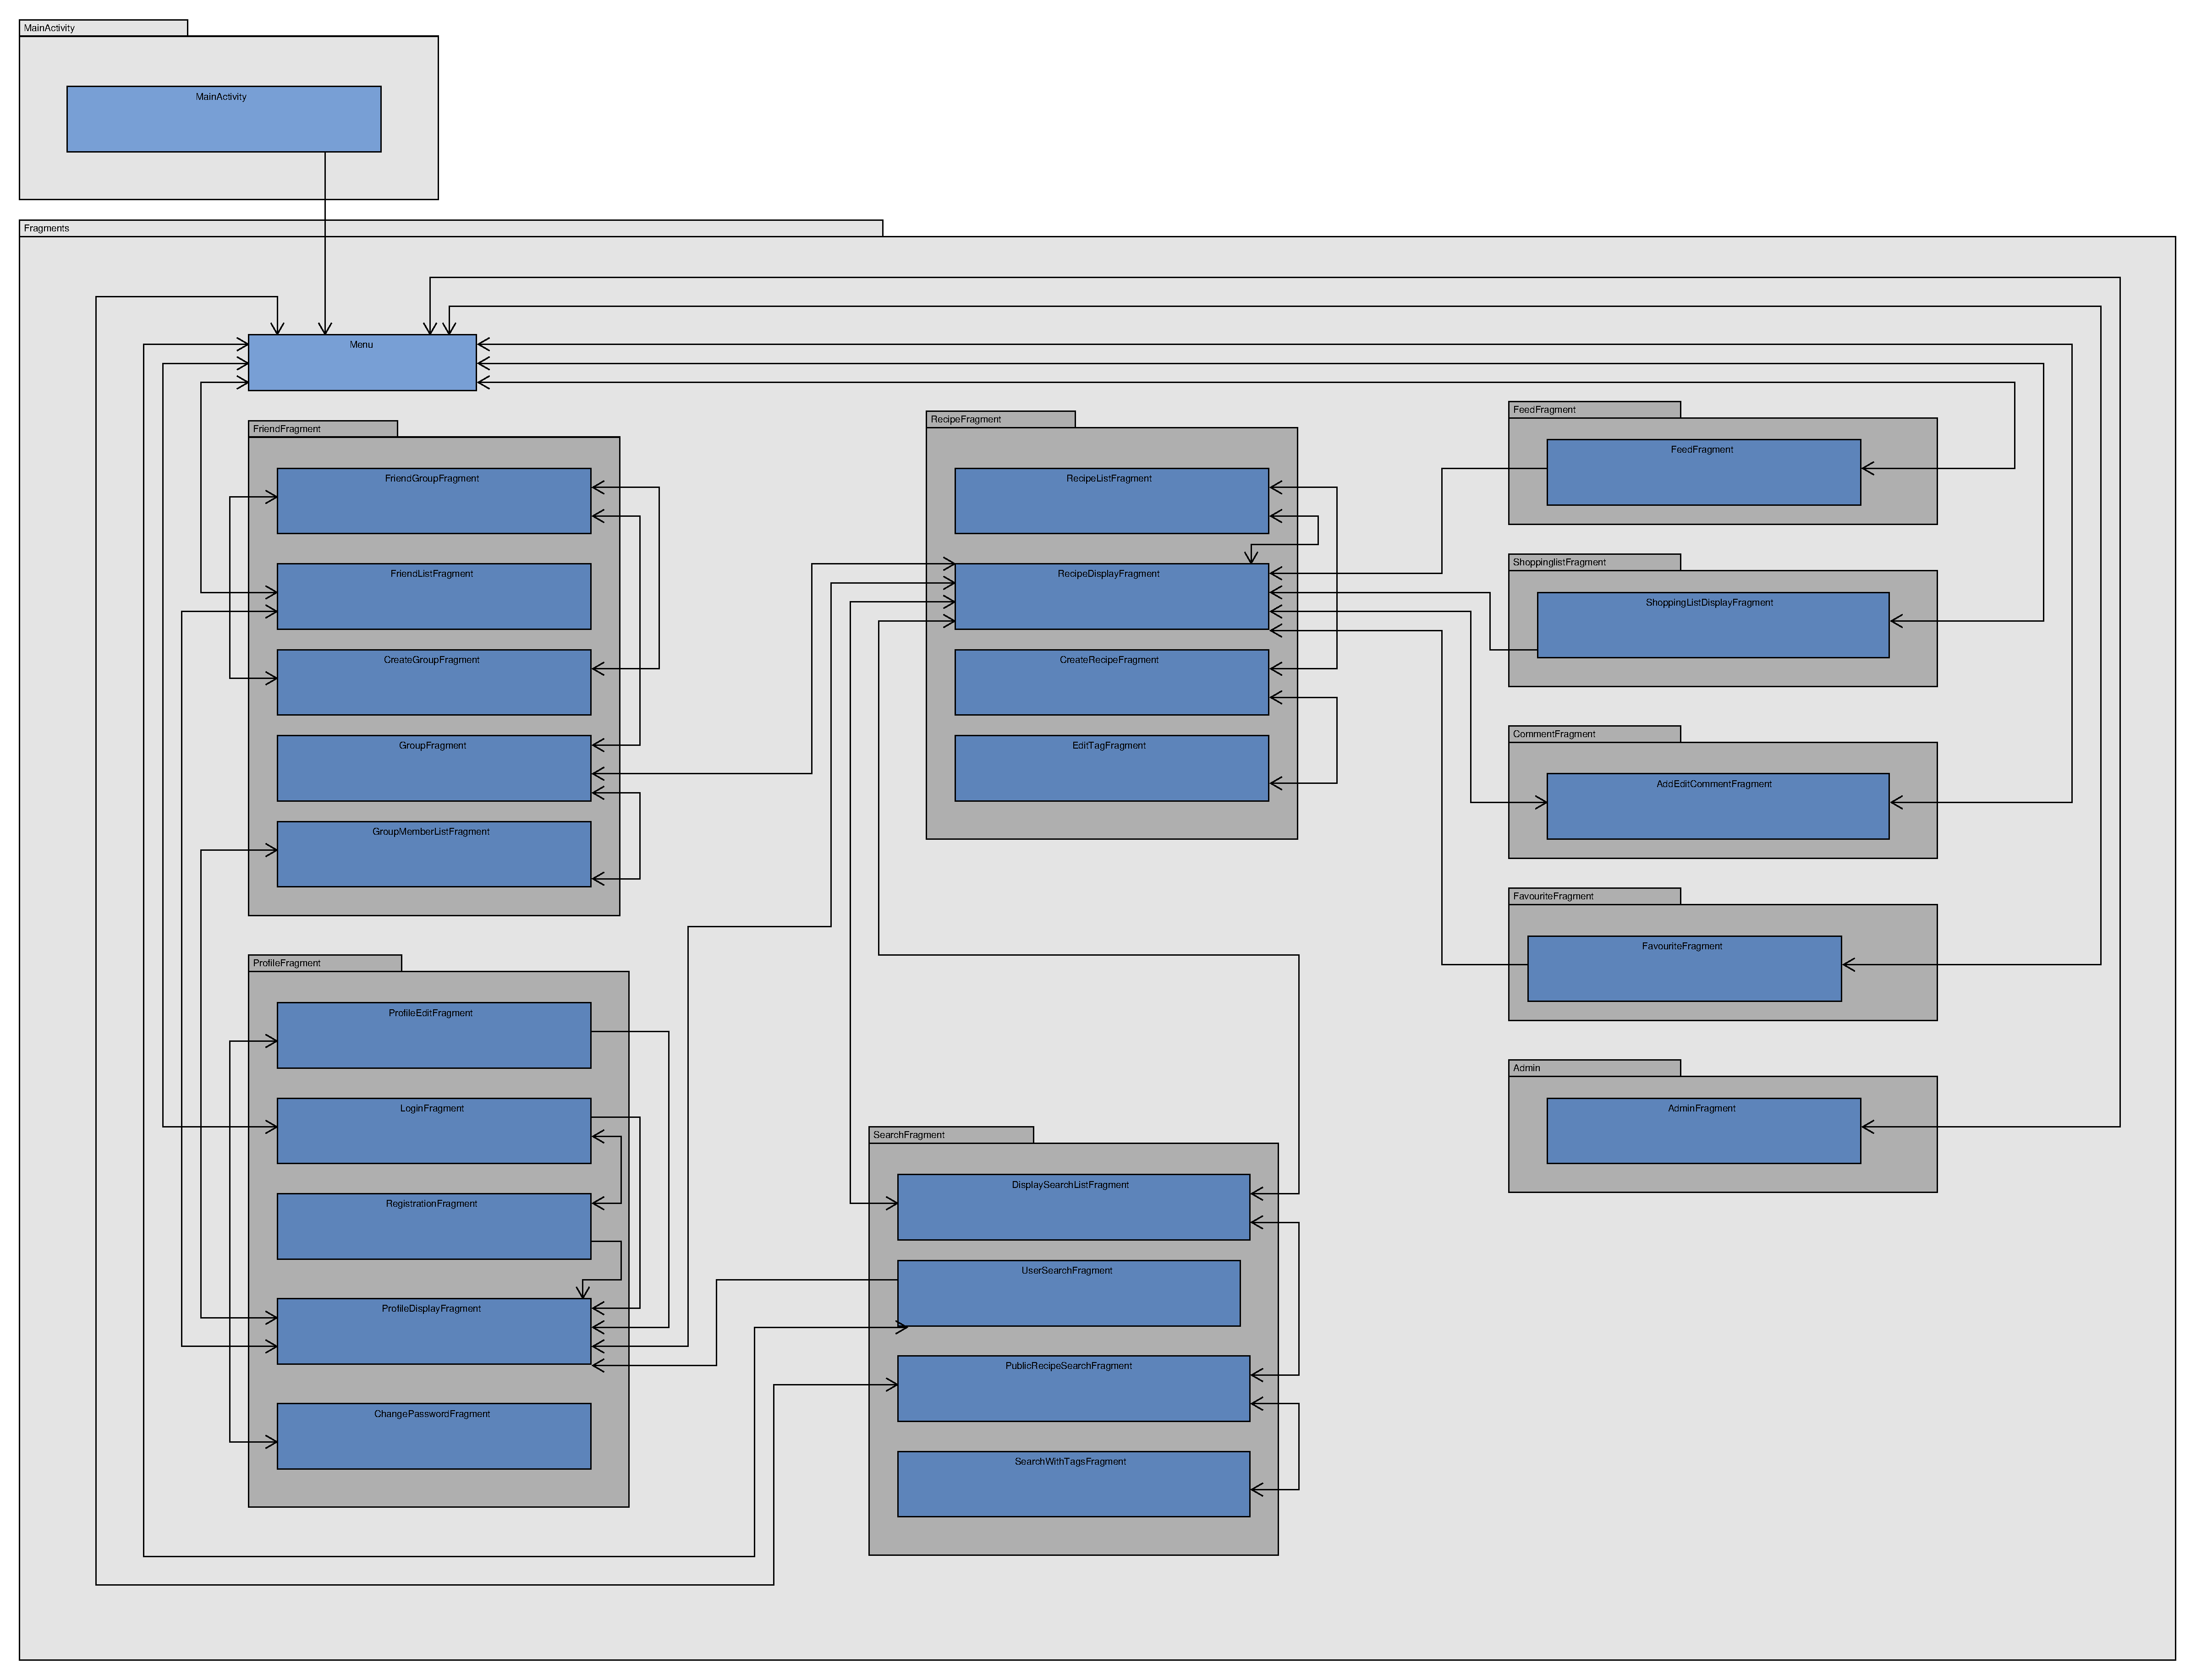
\includegraphics[width=1\textwidth]{pics/viewPackages/ViewPaketmodel_Interaktion.pdf}%
	\caption{Interaktion zwischen den Fragments und der Main-Activity}%
	\label{viewinteract}%
\end{figure}

\subsubsection{FriendFragment Paket}
\begin{figure}[H]
	\centering
	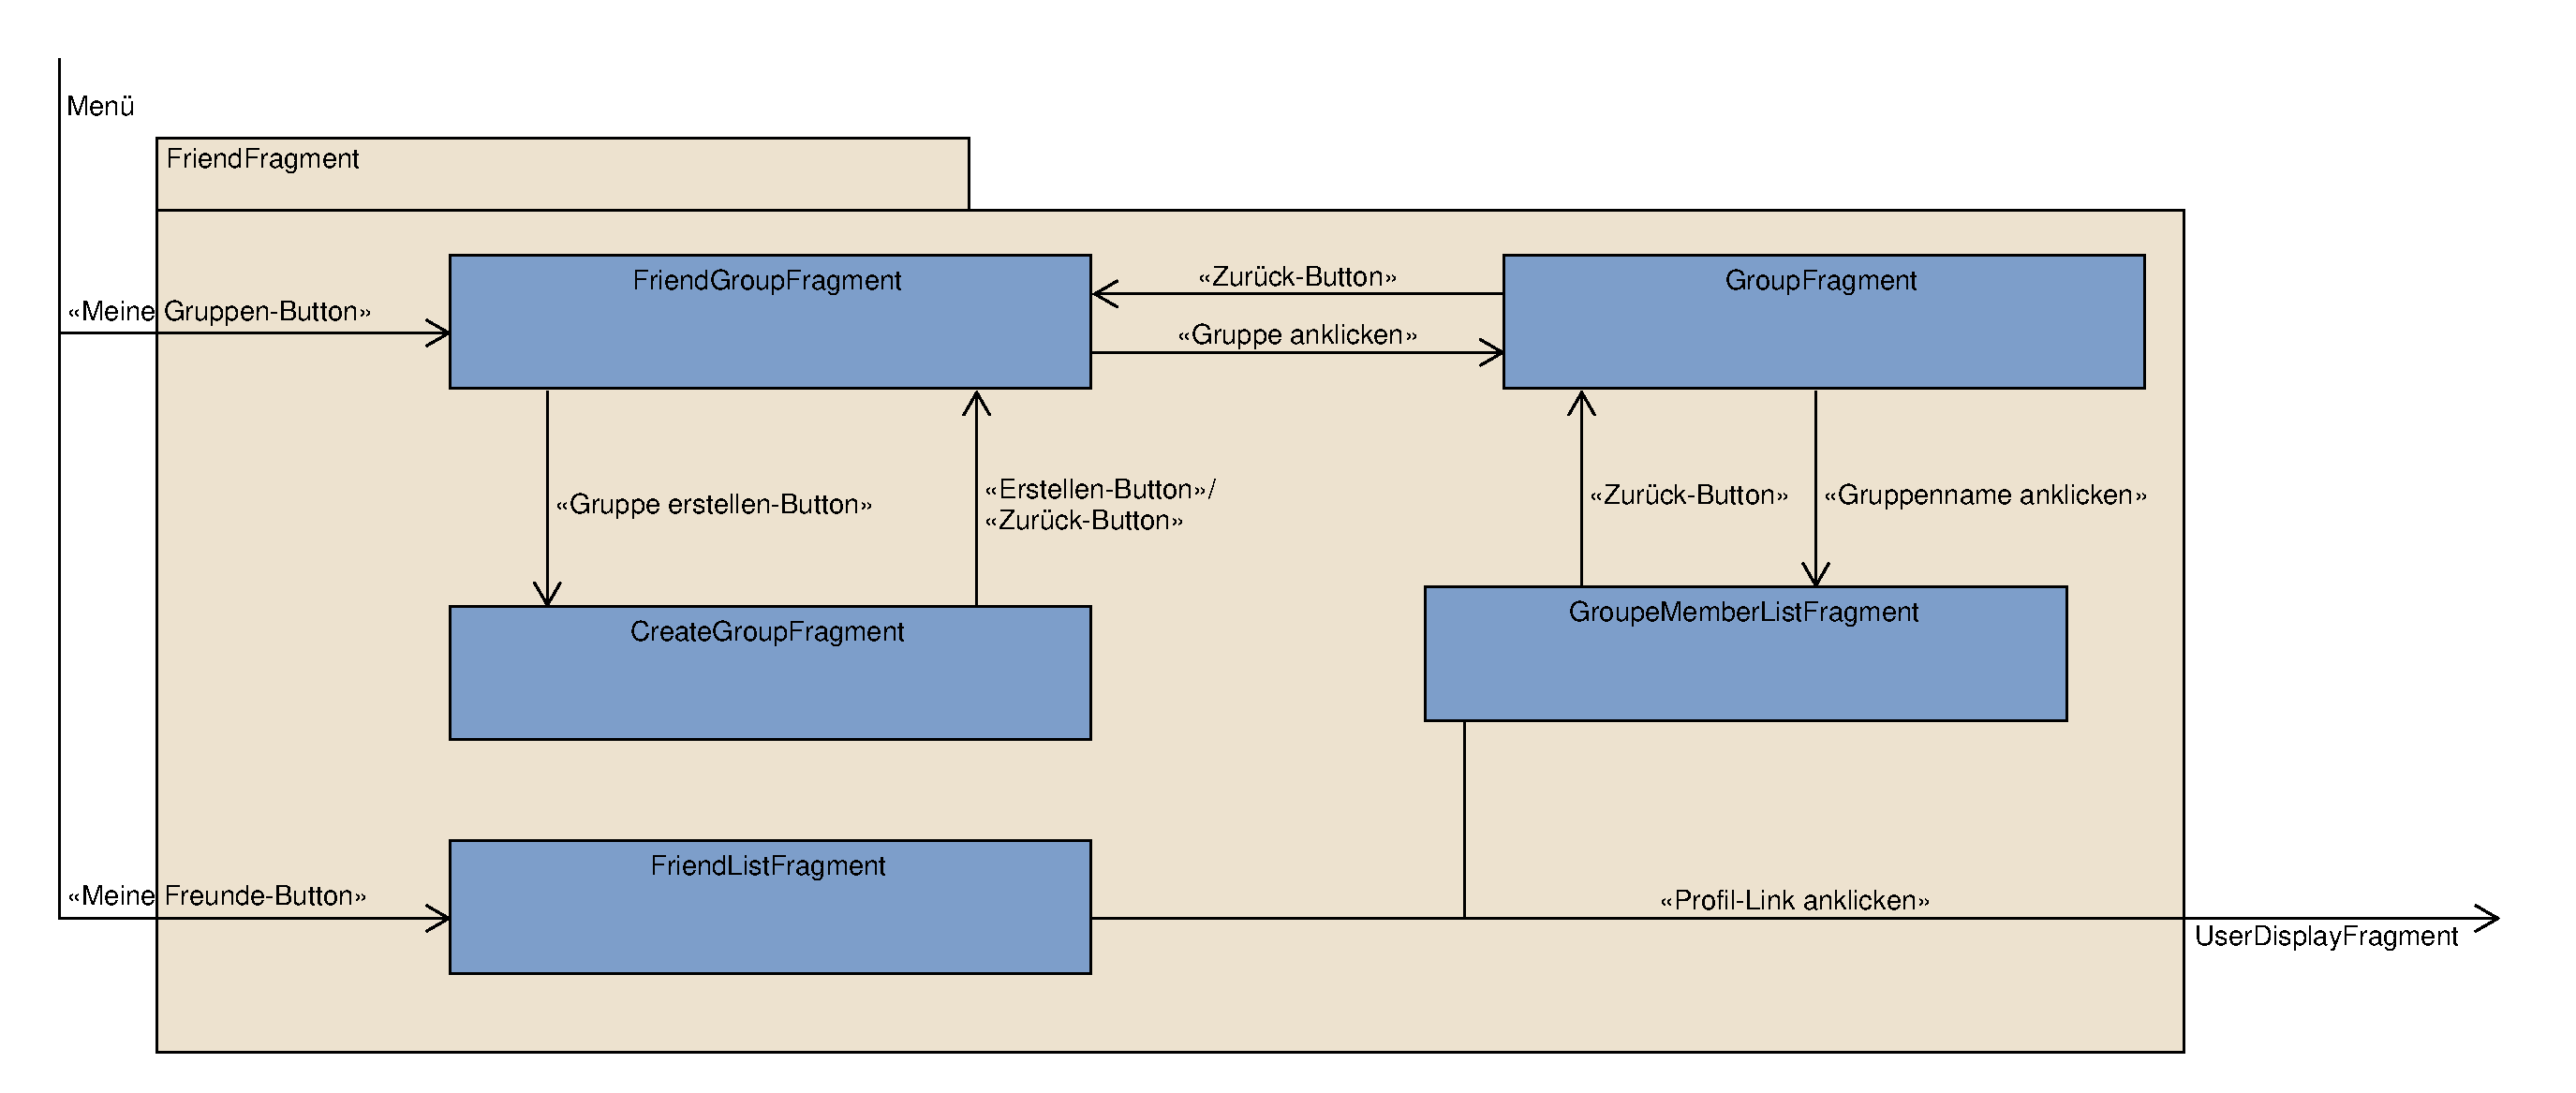
\includegraphics[width=0.8\textwidth]{pics/viewPackages/FriendFragmentPaket.pdf}%
	\caption{FriendFragment Paket}%
	\label{view}%
\end{figure}


Das FriendFragmentPaket ist dafür zuständig, die graphischen Oberflächen der Freunde- und Gruppenverwaltung zu erstellen. 
Sowohl die Übersicht über die Gruppen eines Nutzers, als auch die Liste der Freunde eines Nutzer haben einen eigenen Menüpunkt, deswegen sind diese Fragments über das Appmenü erreichbar.


\subsubsection{RecipeFragment Paket}
\begin{figure}[H]
	\centering
	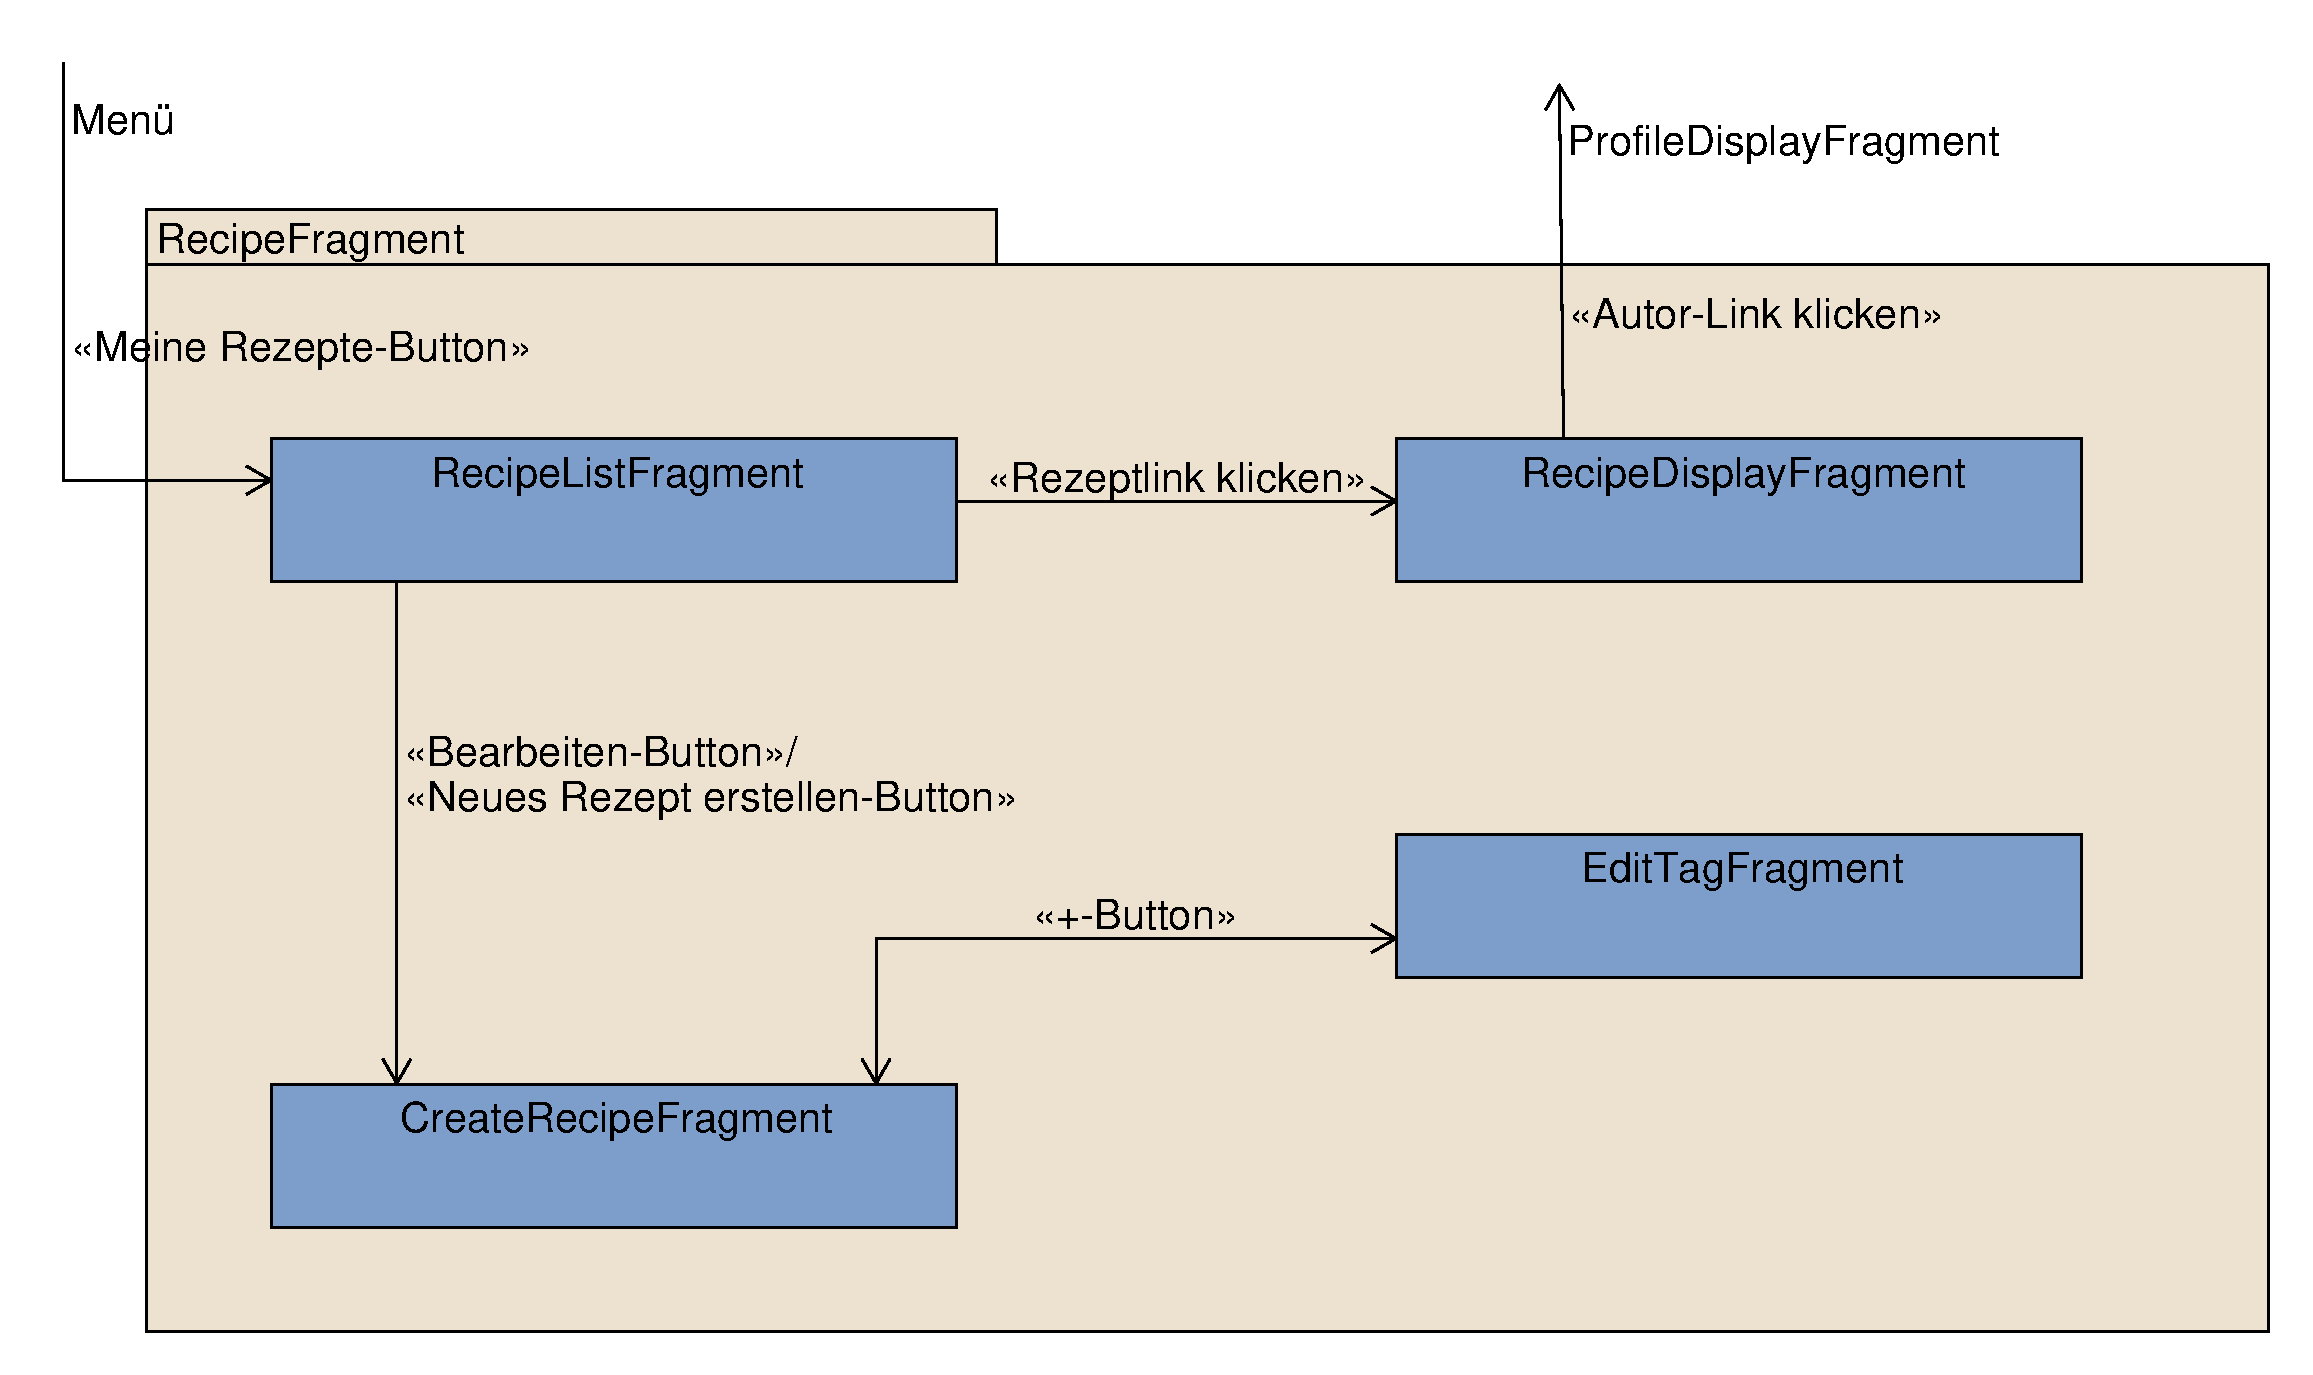
\includegraphics[width=0.8\textwidth]{pics/viewPackages/RecipeFragmentPaket.pdf}%
	\caption{RecipeFragment Paket}%
	\label{view}%
\end{figure}

Das RecipeFragmentPaket ist dafür zuständig die graphischen Oberflächen der Rezeptansichten. 
Wichtig ist die Unterscheidung von öffentlichen und privaten Rezepten. Öffentliche Rezepte haben ein festes Format und haben kein einziges Attribut = null , wobei private Rezepte nicht formatiert sein müssen und leere Attribute haben können. Daher ist die Anzeige der zwei Rezepttypen verschieden. 
Das RecipeListFragment stellt eine Liste der privaten Rezepte eines Autors dar. Es kann über das Appmenü aufgerufen werden.

\subsubsection{ProfileFragment Paket}
\begin{figure}[H]
	\centering
	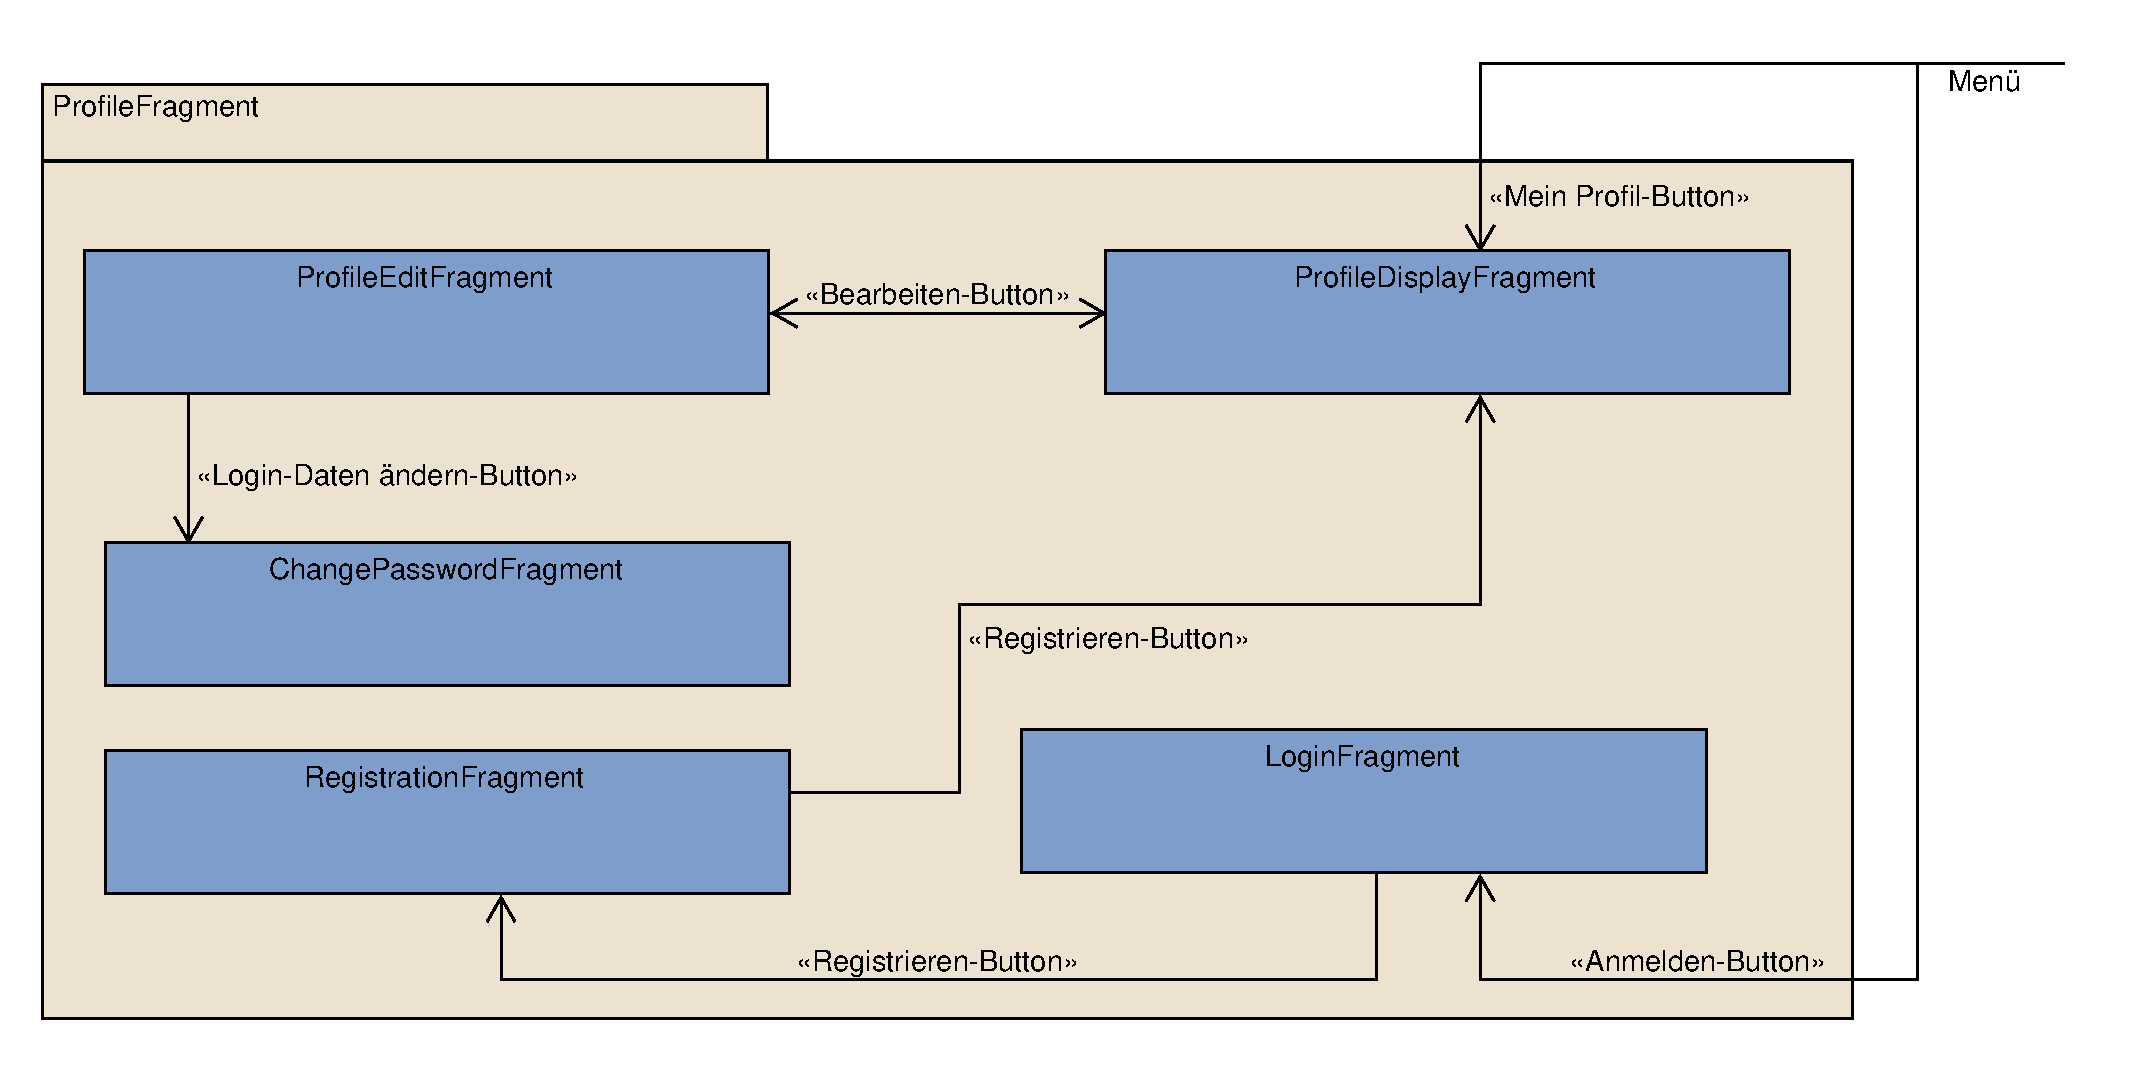
\includegraphics[width=0.8\textwidth]{pics/viewPackages/ProfileFragmentPaket.pdf}%
	\caption{ProfileFragment Paket}%
	\label{view}%
\end{figure}

Das ProfileFragment Paket ist dafür zuständig, eine Graphische Oberfläche für die Nutzerverwaltung bereitzustellen. 
Ein angemeldeter Nutzer kann über das Appmenü das eigene Profil aufrufen. Dann wird das ProfileDisplayFragment angezeigt. Über den "`Bearbeiten"'-Button kommt der Nutzer auf das ProfileEditFragment seines Profils. Möchte er sein Passwort ändern, kann er über den "`Login-Daten ändern"'-Button das ChangePasswordFragment öffnen, um das zu tun.
Das LoginFragment ist über das Appmenü erreichbar. Über den "`Registrieren"'-Button gelangt man auf das RegistrationFragment. Hat sich in diesem Fragment ein Nutzer registriert und klickt auf den "`Registrieren"'-Button, wird er auf das ProfileDisplayFragment seines neu erstellten Profils geleitet.


\subsubsection{SearchFragment Paket}
\begin{figure}[H]
	\centering
	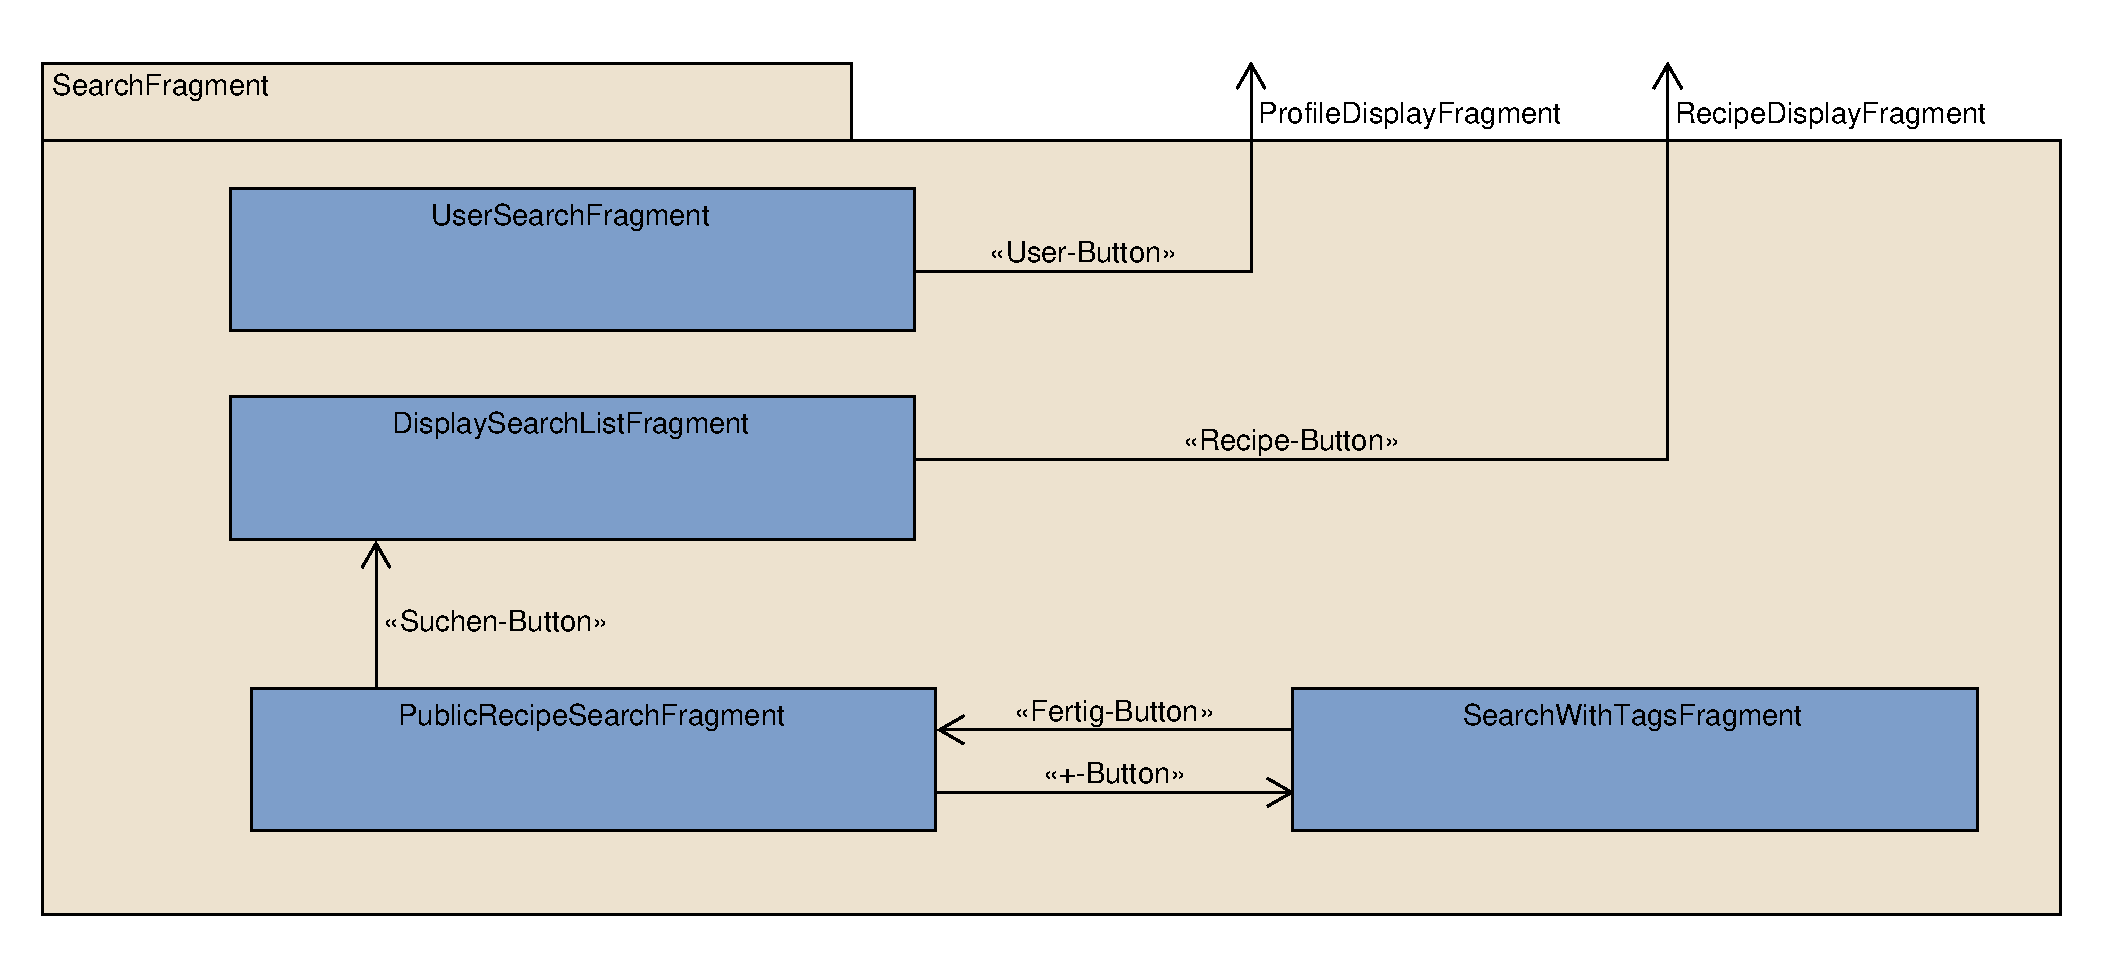
\includegraphics[width=0.8\textwidth]{pics/viewPackages/SearchFragmentPaket.pdf}%
	\caption{SearchFragment Paket}%
	\label{view}%
\end{figure}
Das SearchFragment Paket ist dafür zuständig die 
graphische Oberfläche für die verschiedenen Suchfunktionen
bereit zu stellen. 

\subsubsection{ShoppingListFragment Paket}
\begin{figure}[H]
	\centering
	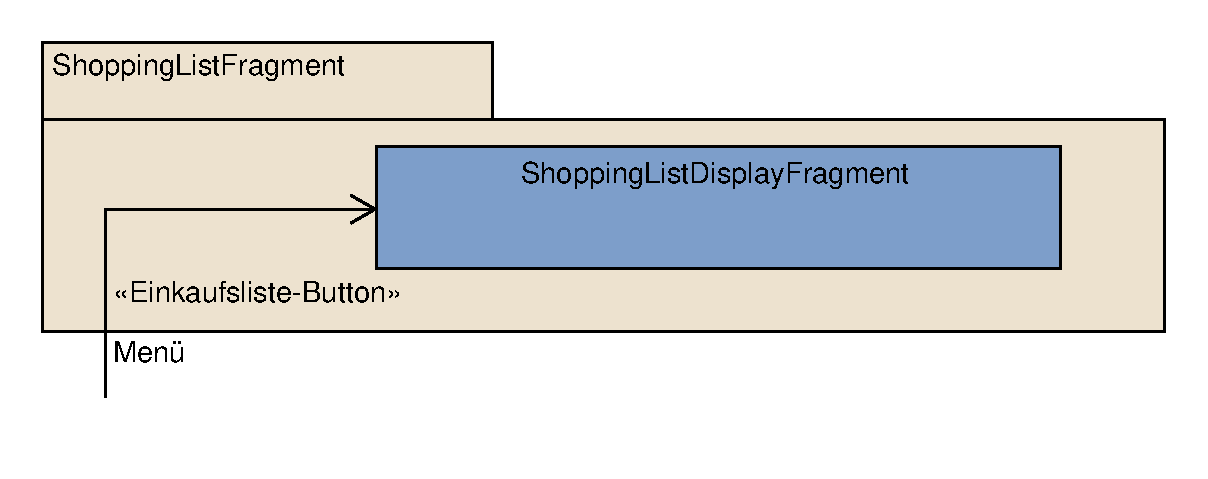
\includegraphics[width=0.8\textwidth]{pics/viewPackages/ShoppinglistFragmentPaket.pdf}%
	\caption{ShoppinglistFragment Paket}%
	\label{view}%
\end{figure}

Das ShoppingListFragment Paket ist dafür zuständig, die Oberfläche
der Einkaufsliste darzustellen. Das Fragment ist über das Appmenü erreichbar.


\subsubsection{FeedFragment Paket}
\begin{figure}[H]
	\centering
	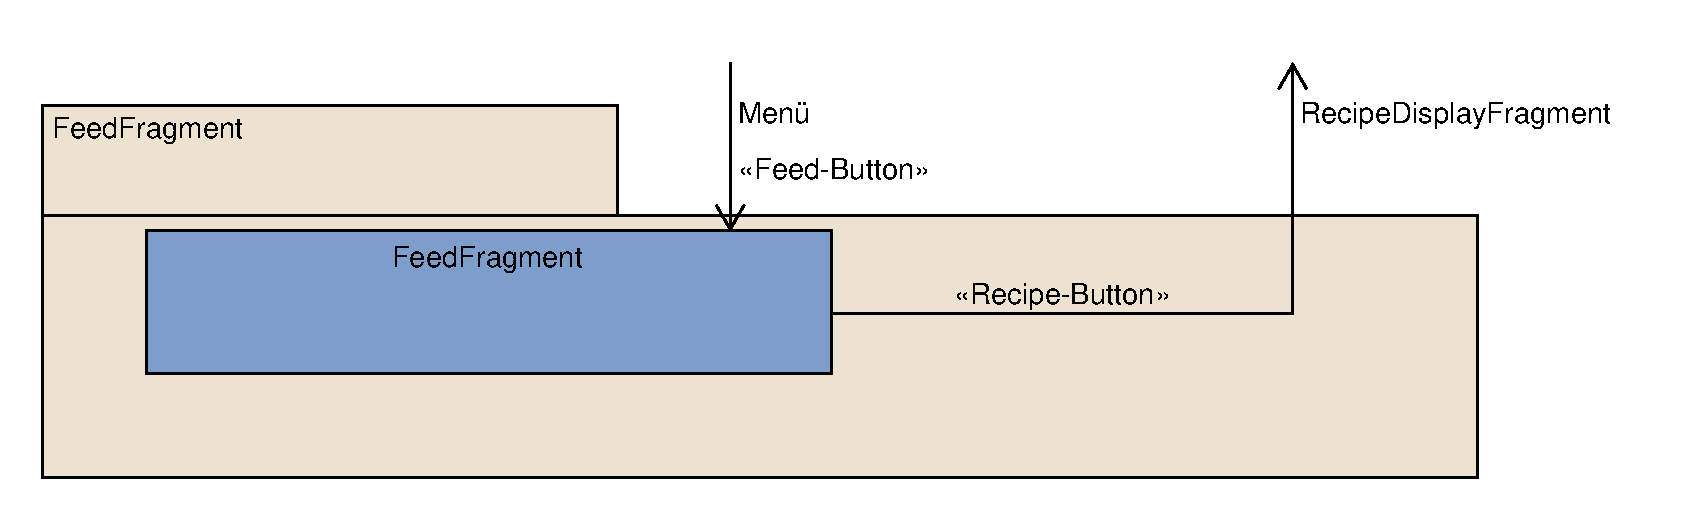
\includegraphics[width=\textwidth]{pics/viewPackages/FeedFragmentPaket.pdf}%
	\caption{FeedFragment Paket}%
	\label{view}%
\end{figure}
Das FeedFragment Paket ist dafür zuständig, die Oberfläche
des Feeds darzustellen. Wenn diese Funktionalität implementiert ist, ist der Feed die Startseite der App und durch das Appmenü erreichbar. Klickt ein User auf einen der Buttons im Feed, so wird er auf das entsprechende Rezept geleitet und das RecipeDisplayFragment öffnet sich.

\subsubsection{FavouriteFragment Paket}
\begin{figure}[H]
	\centering
	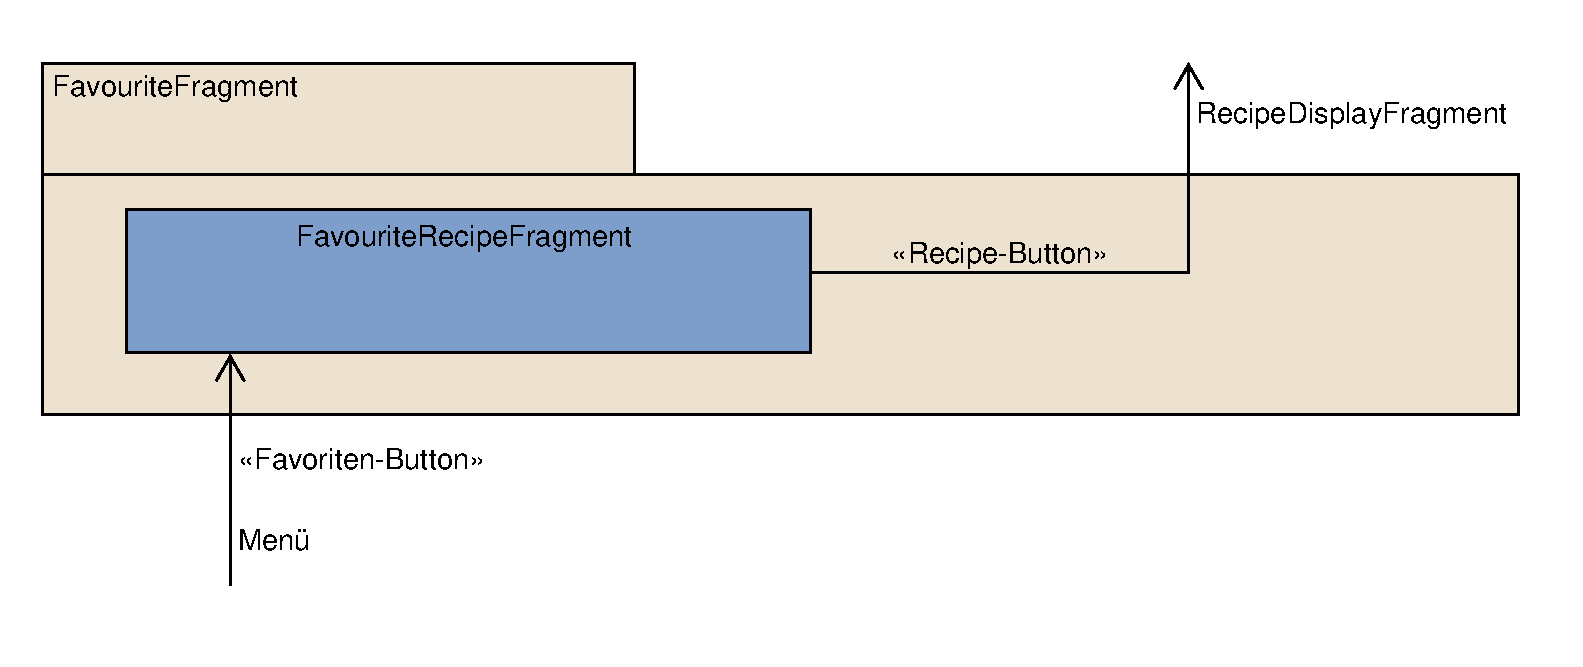
\includegraphics[width=\textwidth]{pics/viewPackages/FavouriteFragmentPaket.pdf}%
	\caption{FavouriteFragment Paket}%
	\label{view}%
\end{figure}

Das FavouriteFragment Paket ist dafür zuständig, die Oberfläche
der Favoritenliste darzustellen.
Diese hat einen eigenen Punkt im Appmenü und ist somit von diesem aus erreichbar. Verlassen wird das Fragment entweder über den "`Zurück"'-Button, oder, indem der Nutzer auf ein angezeigtes Rezept in der Favoritenliste klickt. Dann wird das RecipeDisplayFragment geöffnet.

\subsubsection{AddEditCommentFragment Paket}
\begin{figure}[H]
	\centering
	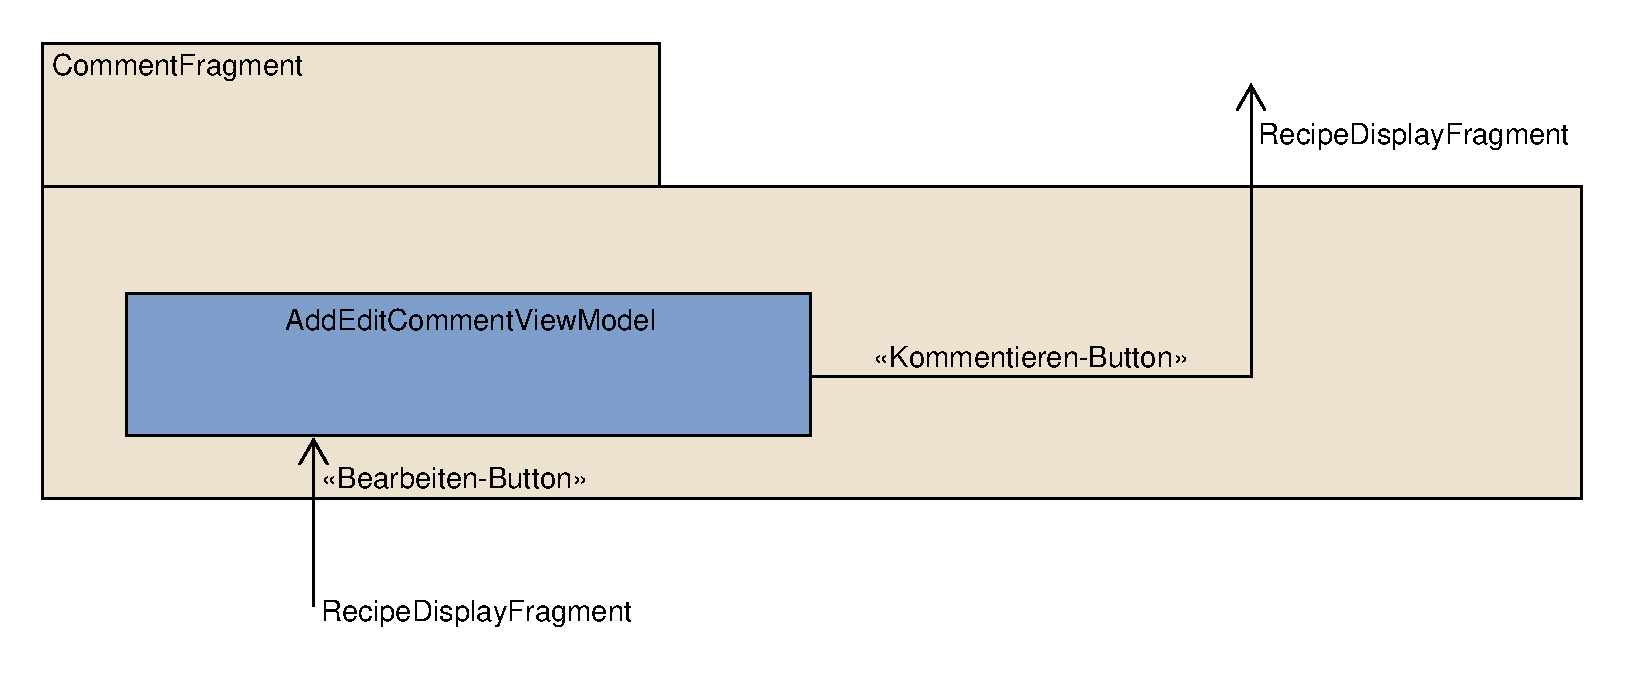
\includegraphics[width=\textwidth]{pics/viewPackages/CommentFragmentPaket.pdf}%
	\caption{FavouriteFragment Paket}%
	\label{view}%
\end{figure}
Das AddEditCommentFragment Paket ist dafür zuständig, die Oberfläche
der Kommentarbearbeitung darzustellen. Das Fragment wird aufgerufen, wenn im RecipeDisplayFragment ein angemeldeter Nutzer bei einem seiner eigens erstellten Kommentare auf "`bearbeiten"' drückt, oder wenn ein angemeldeter Nutzer auf den "`Kommentar schreiben"'-Button drückt. 
Wird der "`kommentieren"'-Button gedrückt, so wird das vorherige RecipeDisplayFragment wieder angezeigt.

\subsubsection{AdminFragment Paket}
\begin{figure}[H]
	\centering
	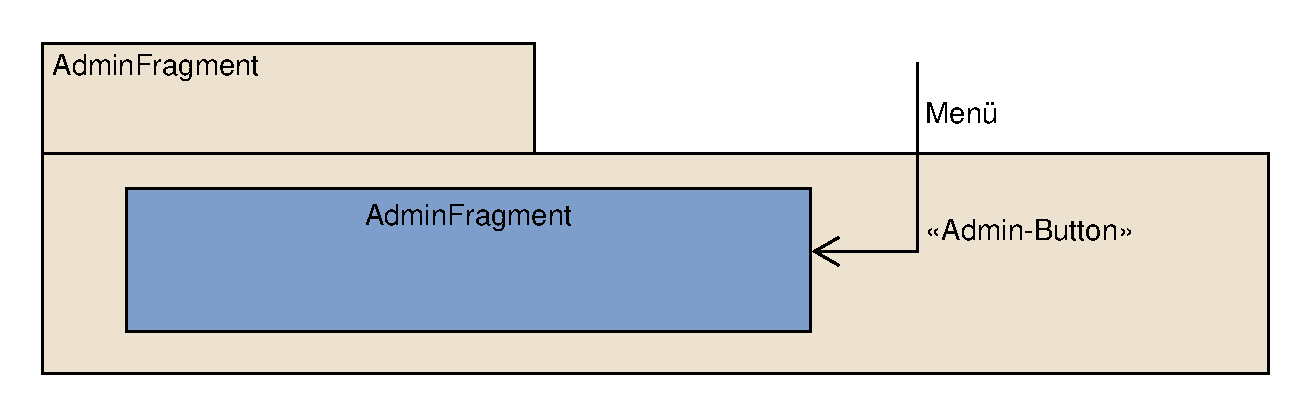
\includegraphics[width=\textwidth]{pics/viewPackages/AdminFragmentPaket.pdf}%
	\caption{AdminFragment Paket}%
	\label{view}%
\end{figure}
Das AdminFragment Paket ist dafür zuständig, die Oberfläche
des Admins darzustellen. Über diese hat der Admin die Möglichkeit gemeldete Rezepte, Nutzer, oder Gruppen manuell zu überprüfen und zu entfernen. Ist ein Nutzer als Admin angemeldet, so ist dieses Fragment über das Appmenü aufrufbar.


\subsection{ViewModel}

\begin{figure}[H]
	\centering
	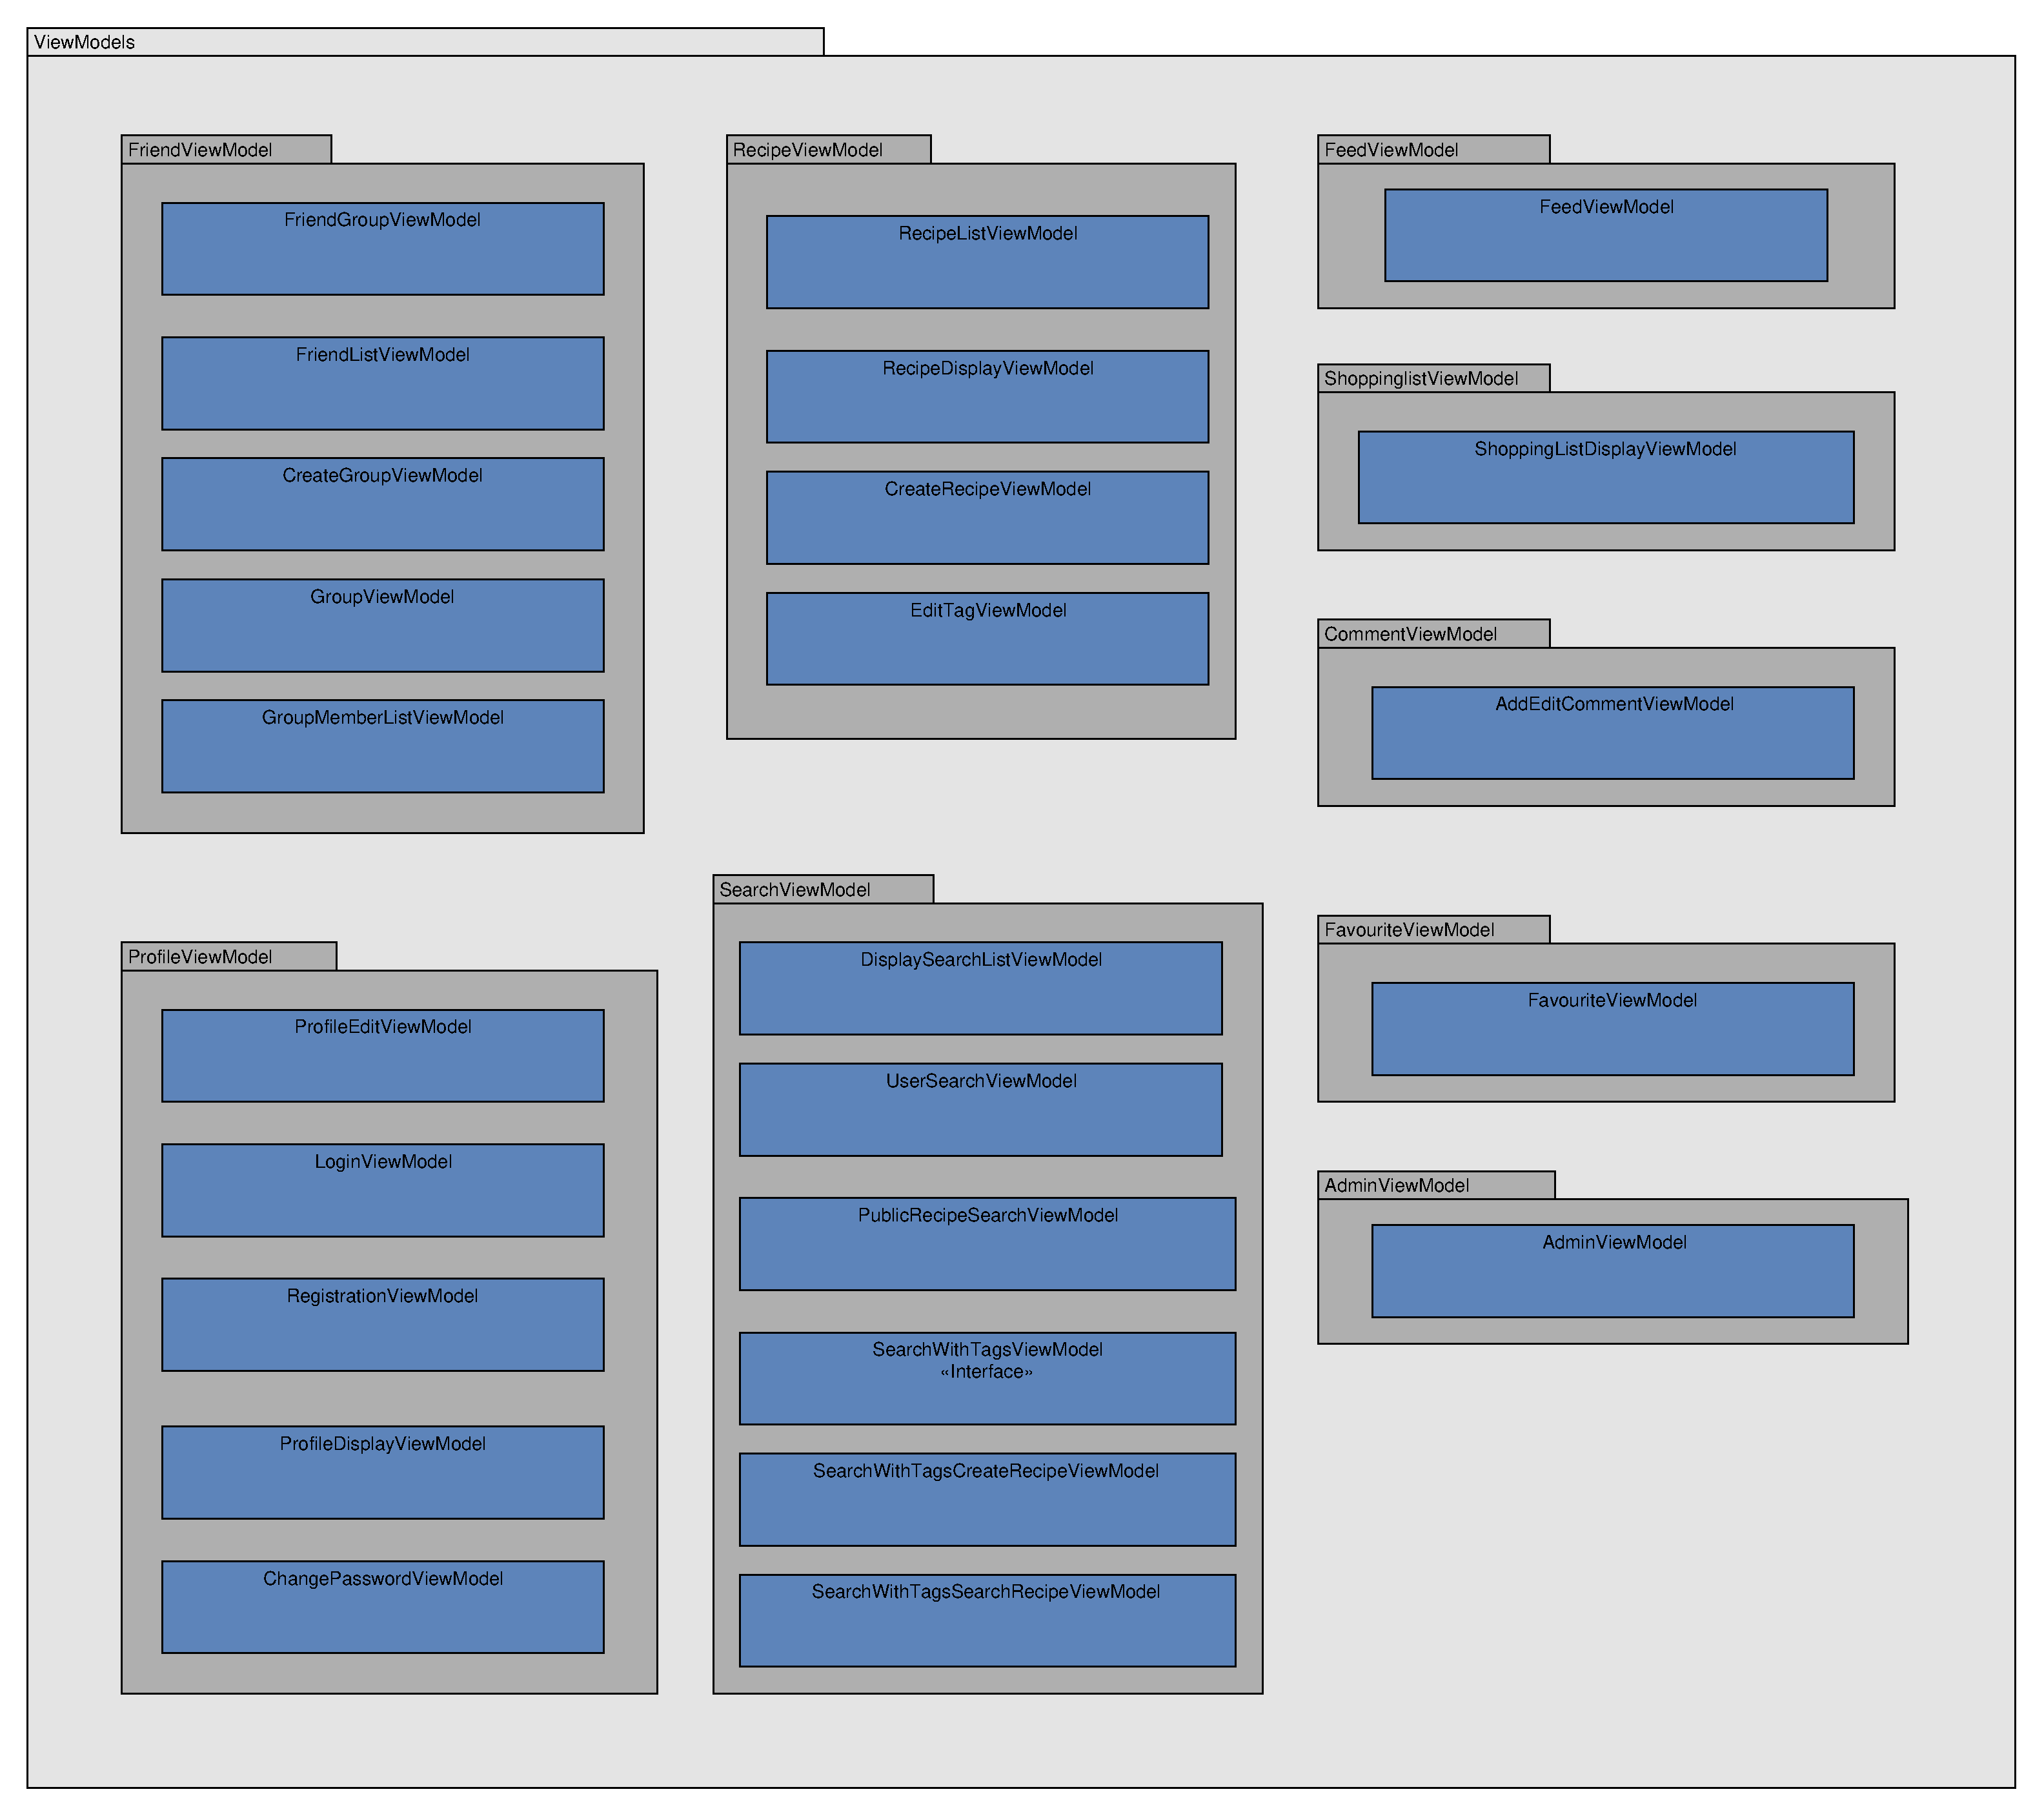
\includegraphics[width=\textwidth]{pics/viewModel/ViewModelPackages.pdf}%
	\caption{Die Packages mit enthaltenen ViewModel-Klassen}%
	\label{vmpackages}%
\end{figure}

An sich sieht das ViewModel-Paket von der Struktur her analog so aus, wie die View-Struktur, da jedes Fragment ein ViewModel benötigt. Das SearchWithTagsFragment ist die einzige Ausnahme, da es von zwei verschiedenen Fragments aus aufgerufen wird und deswegen unterschiedlicher Funktionalitäten bedarf (mehr dazu in Kapitel 5.2). Was auch anders ist, sind die Verbindungen. Die ViewModels haben untereinander keinerlei Interaktion, sondern geben Daten und Anfragen durch Befehle an das Repository zu den Datenquellen durch. Jede VM-Klasse hat also eine Verbindung zum Repository.

\subsection{Domain Layer}

\subsubsection{Domain Entities}

\begin{figure}[H]
	\centering
	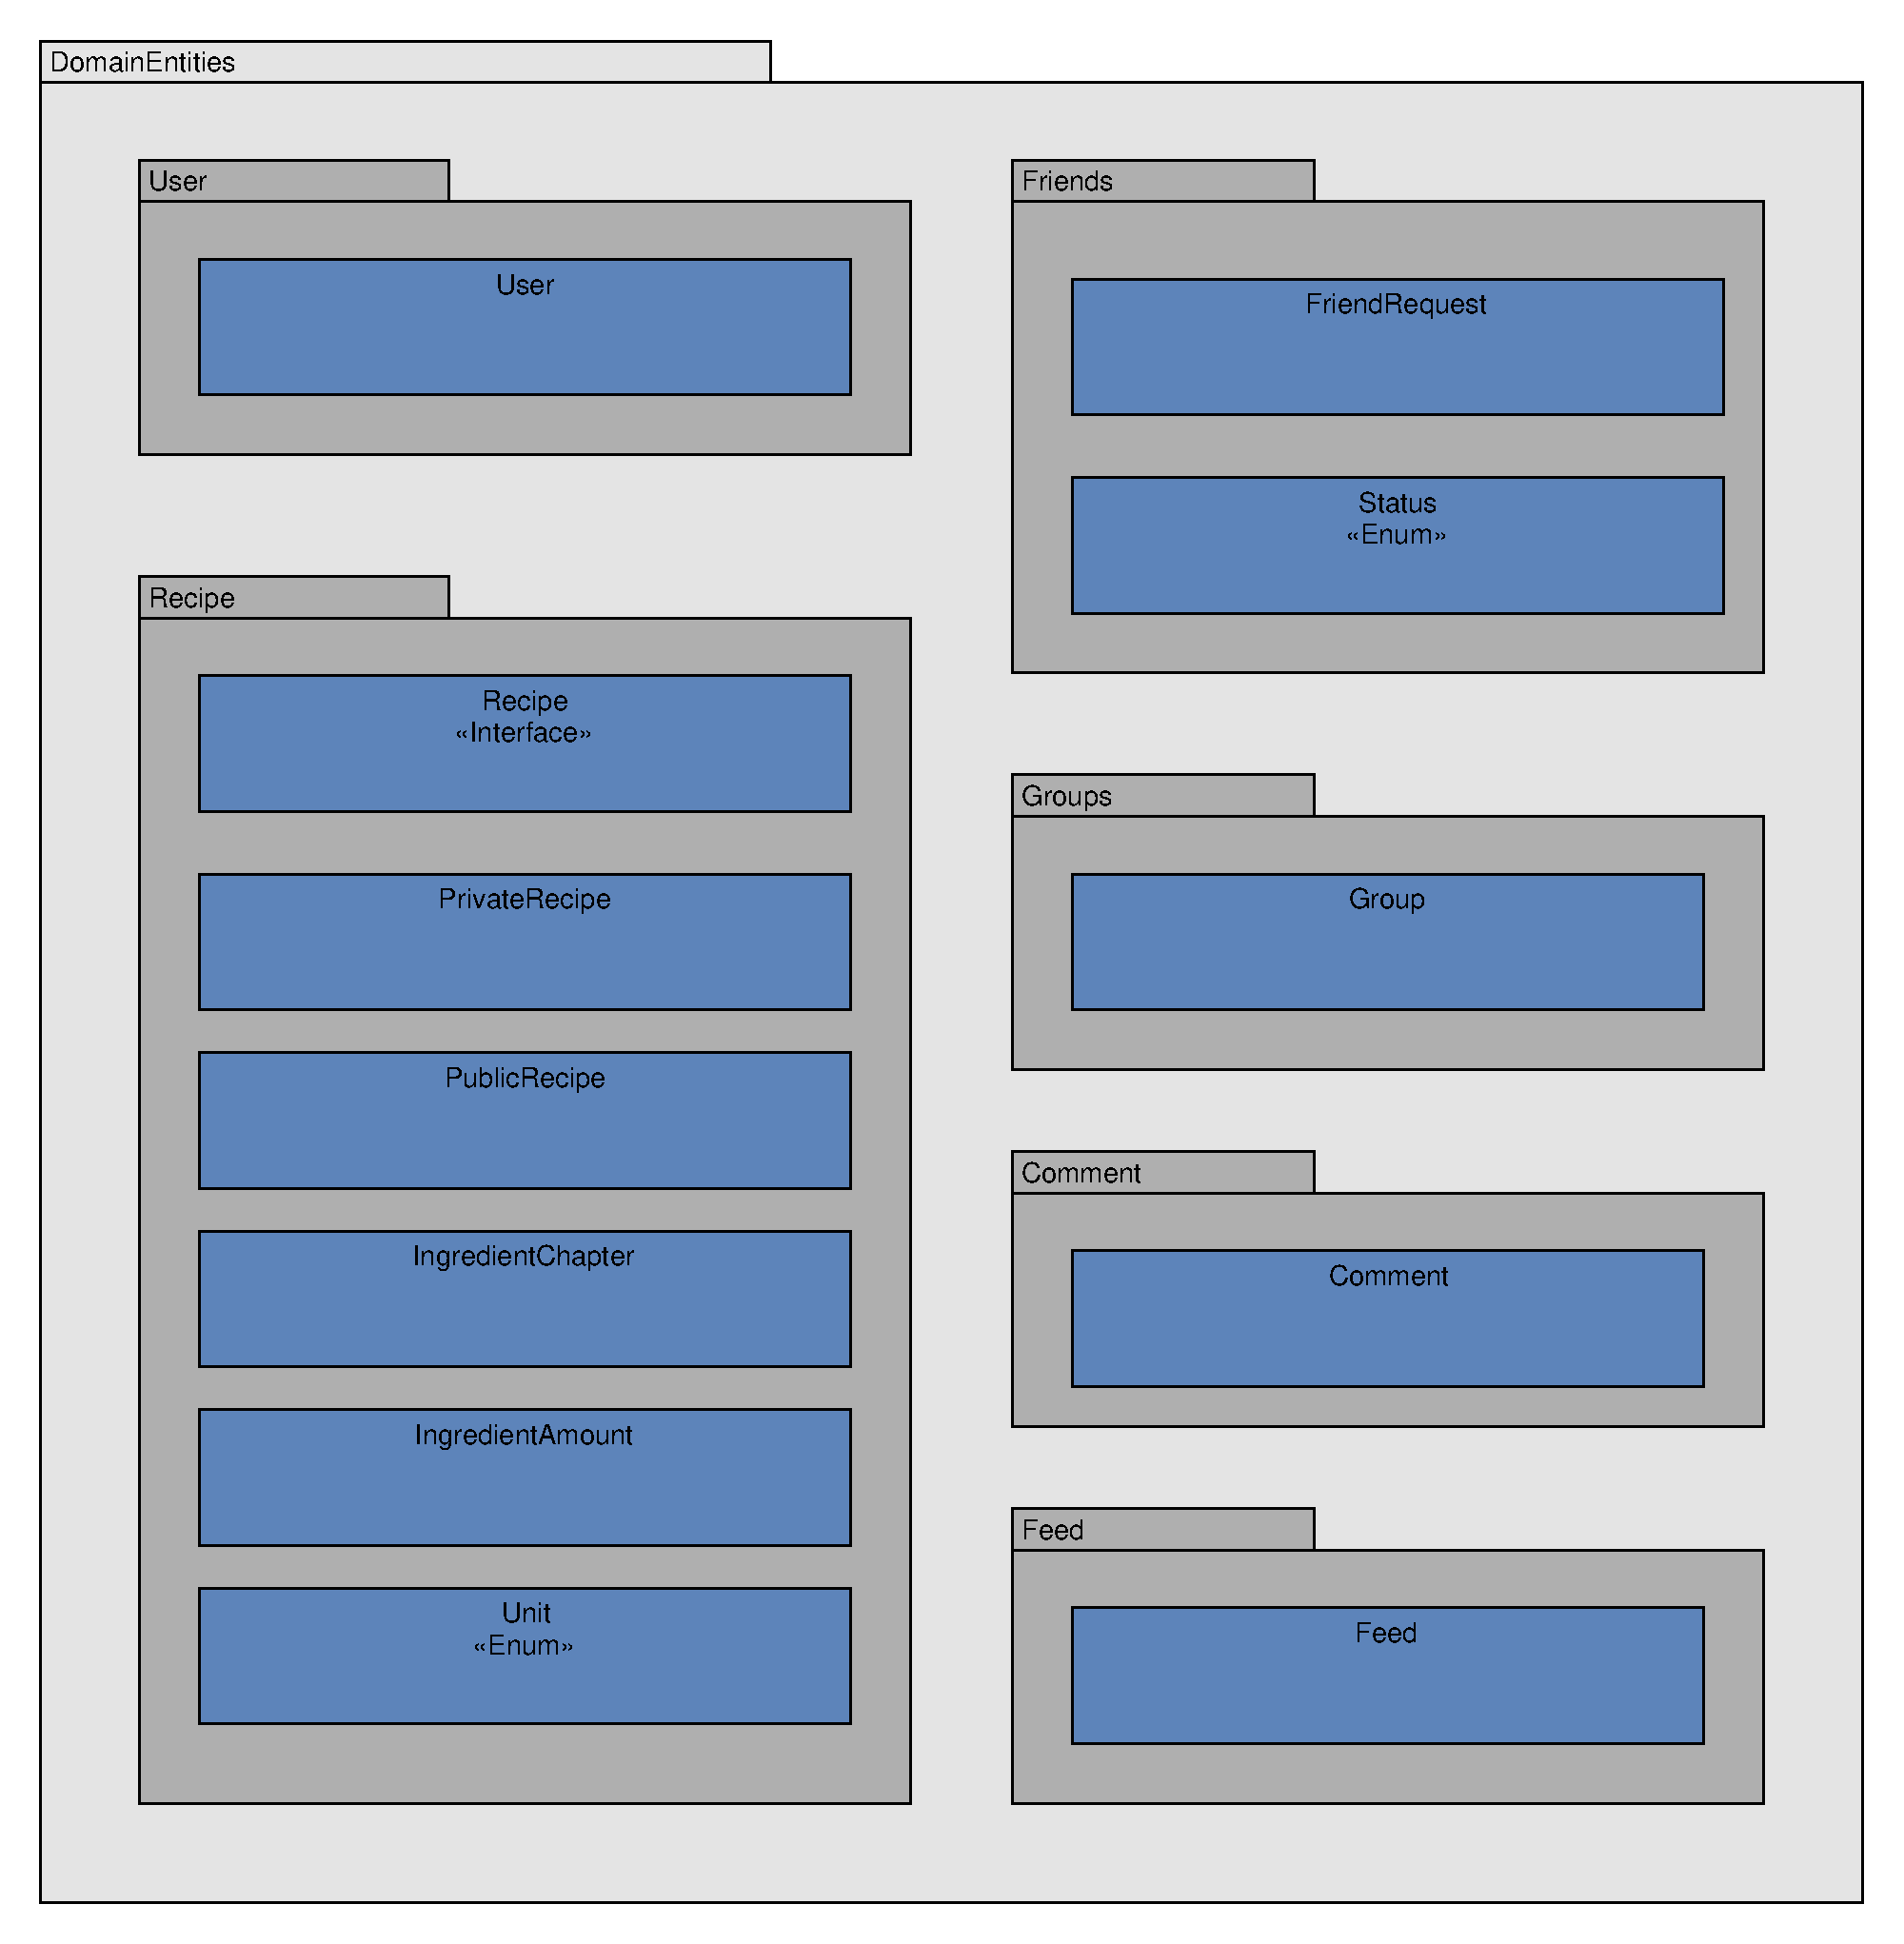
\includegraphics[width=\textwidth]{pics/EntityPackage.pdf}%
	\caption{Das Domain Entity-Paket mit Klassen}%
	\label{domain}%
\end{figure}

Die Domain Entities stellen auf der Appseite den Kern des Models dar. Sie liegen in einem Paket und interagieren miteinander, aber nicht mit Klassen außerhalb ihres Paketes. Die Interaktion der Entities ist in Kapitel 6.1 ausführlicher erklärt.

\subsubsection{Domain Layer Interfaces}

\begin{figure}[H]
	\centering
	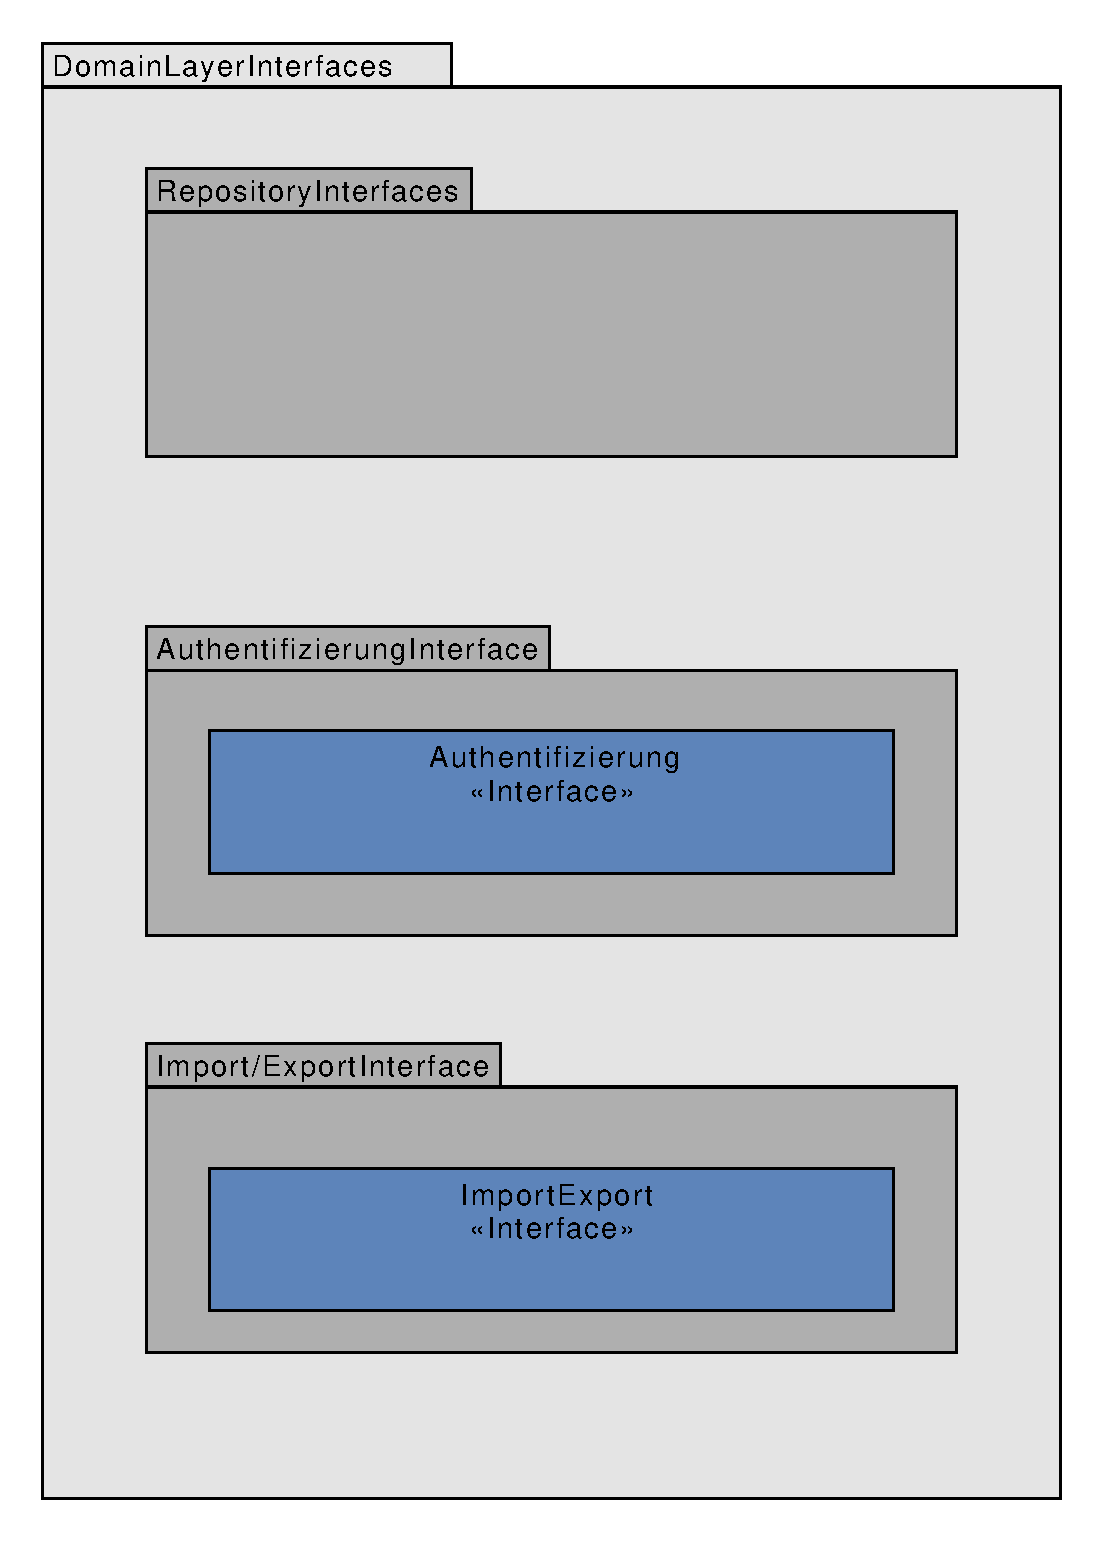
\includegraphics[width=\textwidth]{generatedpics/DomainLayerInterfaces.pdf}%
	\caption{Die Interfaces des Domain Layers}%
	\label{interf}%
\end{figure}

Im Domain Layer liegen einige Interfaces, die für verschiedene Funktionalitäten gebraucht werden. Unter anderem sind die Repository-Interfaces, das ImportExport-Interface und das Authentifizierungs-Interface hier enthalten. Diese bieten Schnittstellen, um Bibliotheken oder eigene Funktionale Klassen (zB. das Repository) gekapselt einzubinden.
Im Repository-Interfaces-Package sind verschiedene Interfaces enthalten. Für jede Klasse im Repository (siehe folgenden Abschnitt), ist ein Interface im Package enthalten, welches die Methoden und Attribute der Klasse vorgibt.

\subsection{Data Layer}

\begin{figure}[H]
	\centering
	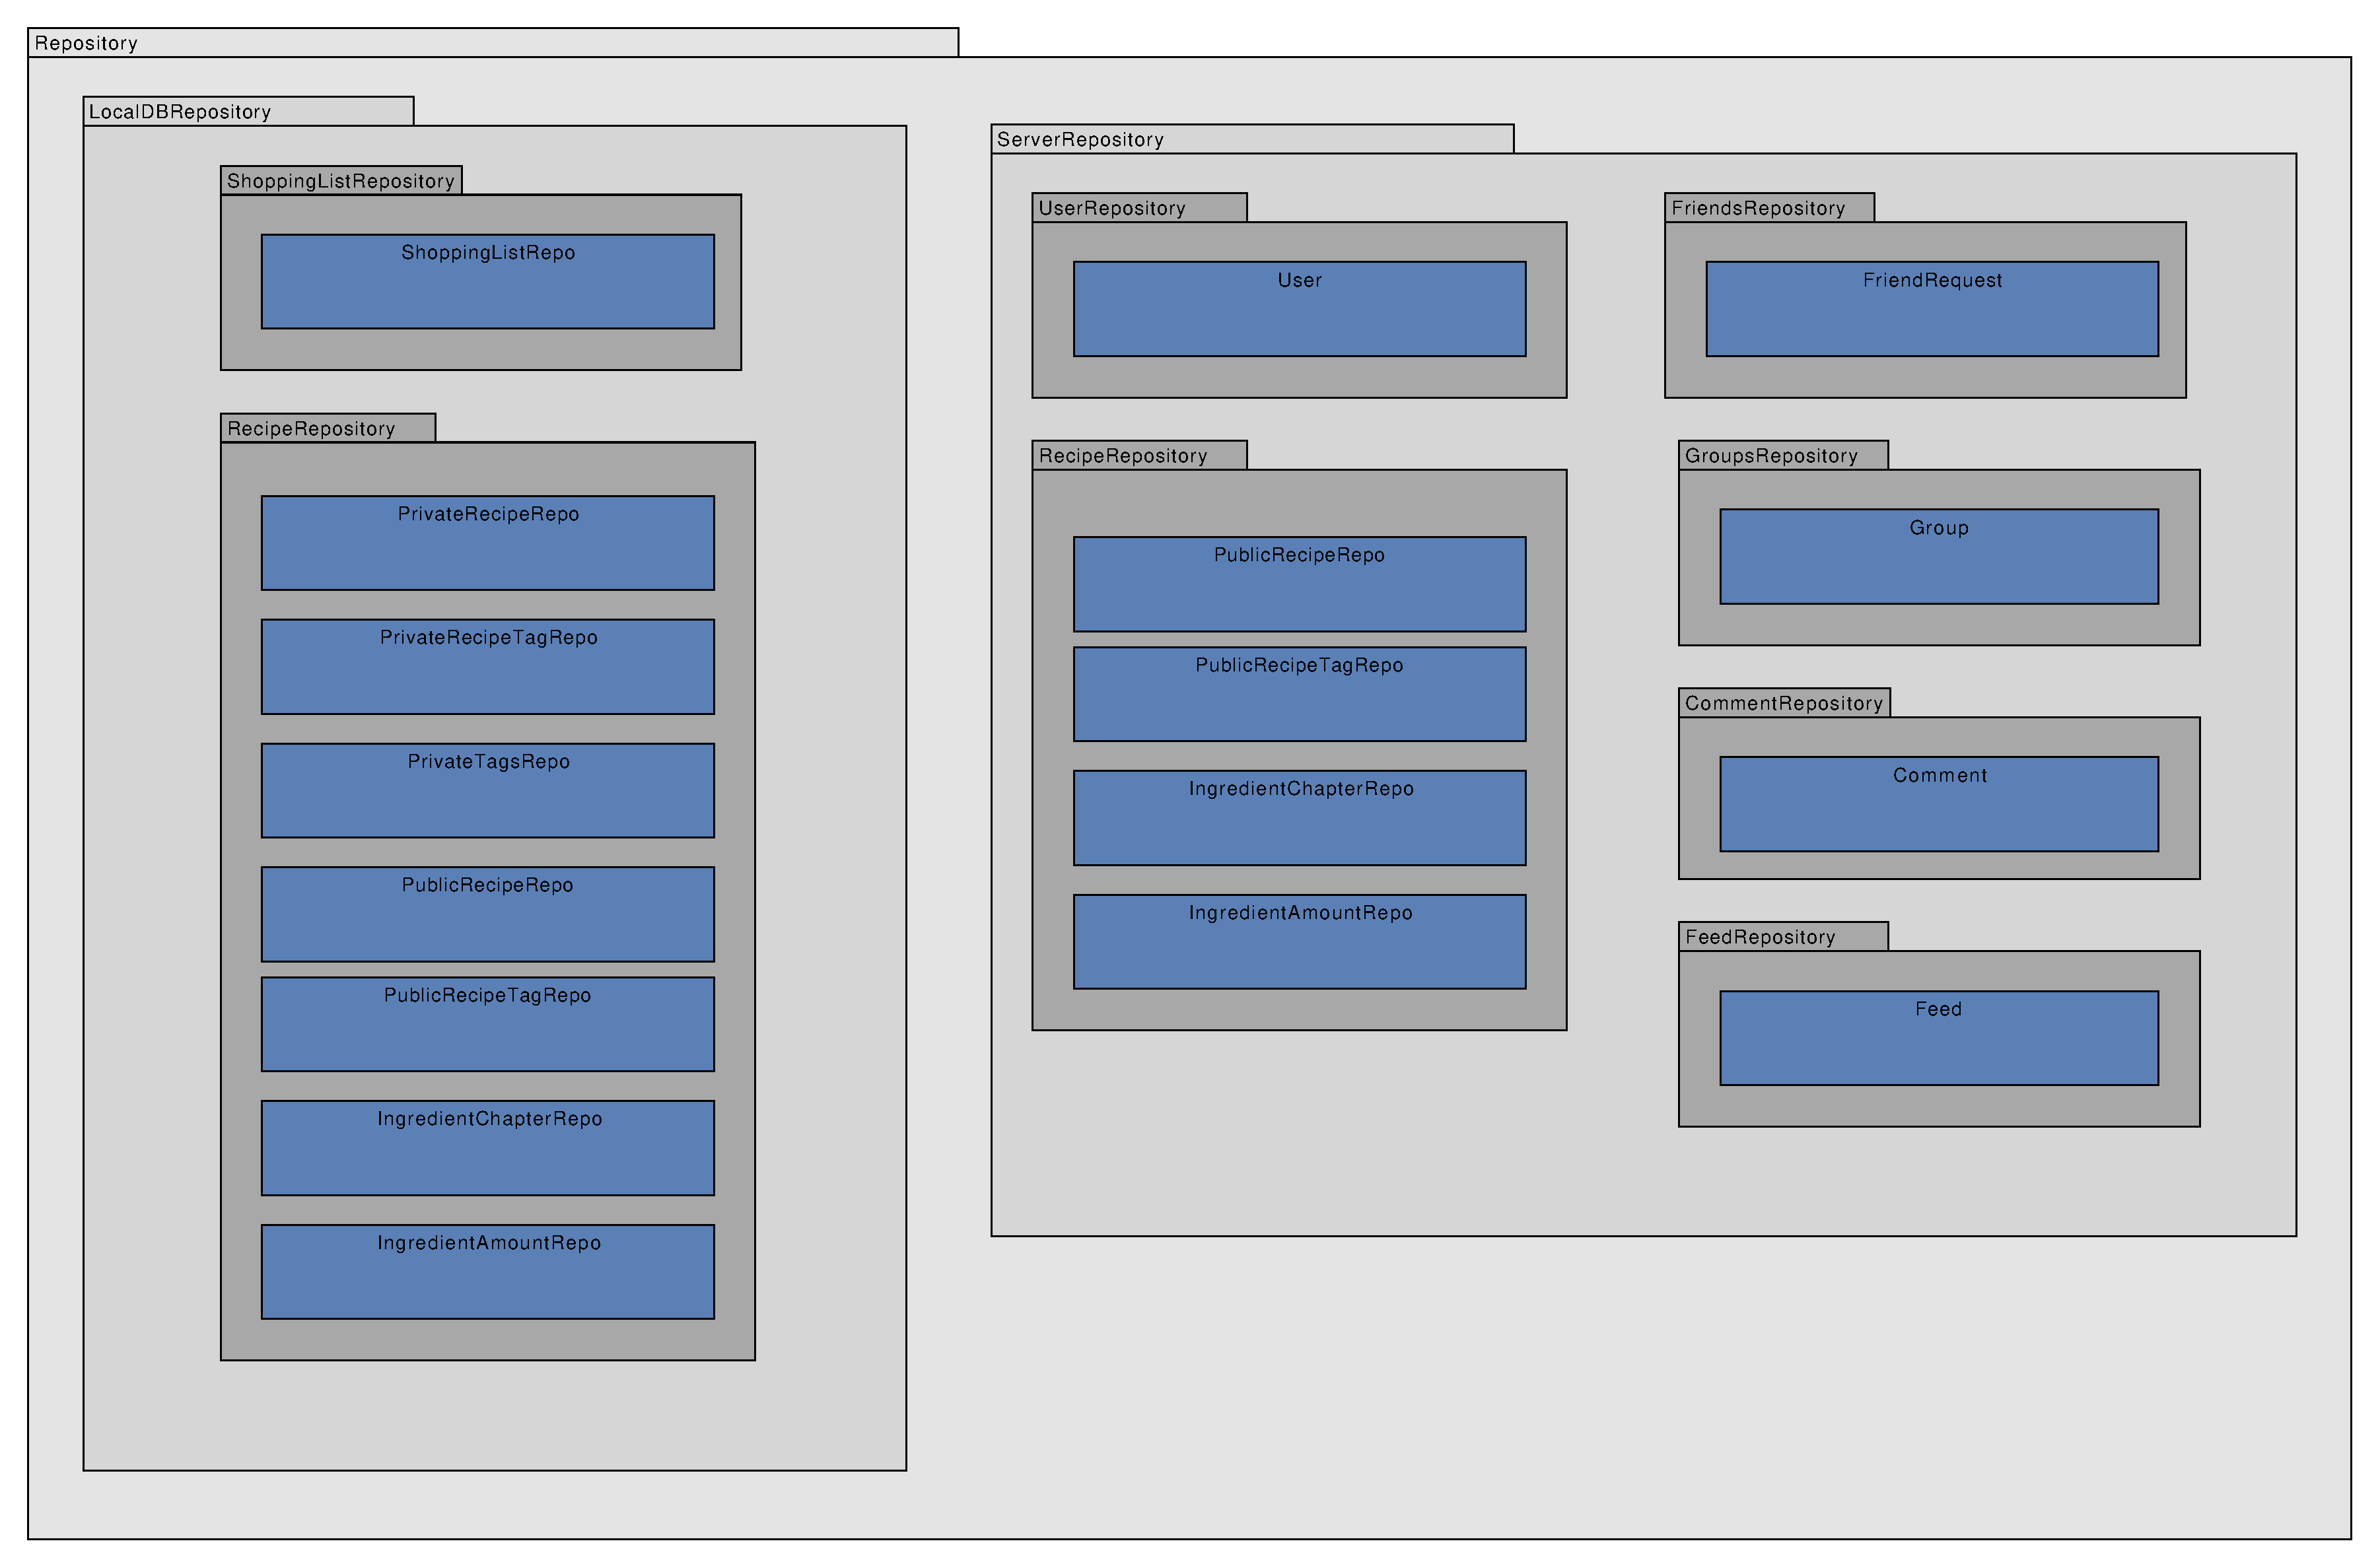
\includegraphics[width=\textwidth]{generatedpics/RepositoryPackage.pdf}%
	\caption{Das Paket mit Klassen des Repositories}%
	\label{repo}%
\end{figure}

Das Repository enthält für fast jede Domain Entity eine Klasse, in der Methoden zur Datenverwaltung dieser Entity enthalten sind. Es ist aufgeteilt in ein Package für die lokale SQLite Room-Datenbank und eines für den Webserver.

\section{Server}

\subsection{Api und Model Pakete}

In der Abbildung \ref{serverapidb} werden alle Pakete und Klassen aufgelistet, welche für die Kommunikation mit den Clients (Api/Controller), behandeln von den Anfragen (Services) und den Zugriff auf die Datenbank (Dao und Model) zuständig sind. Die DTOs sind die Klassen bzw. Objekte, welche über das Netzwerk zwischen Client und Server versendet werden.

\begin{figure}[H]
	\centering
	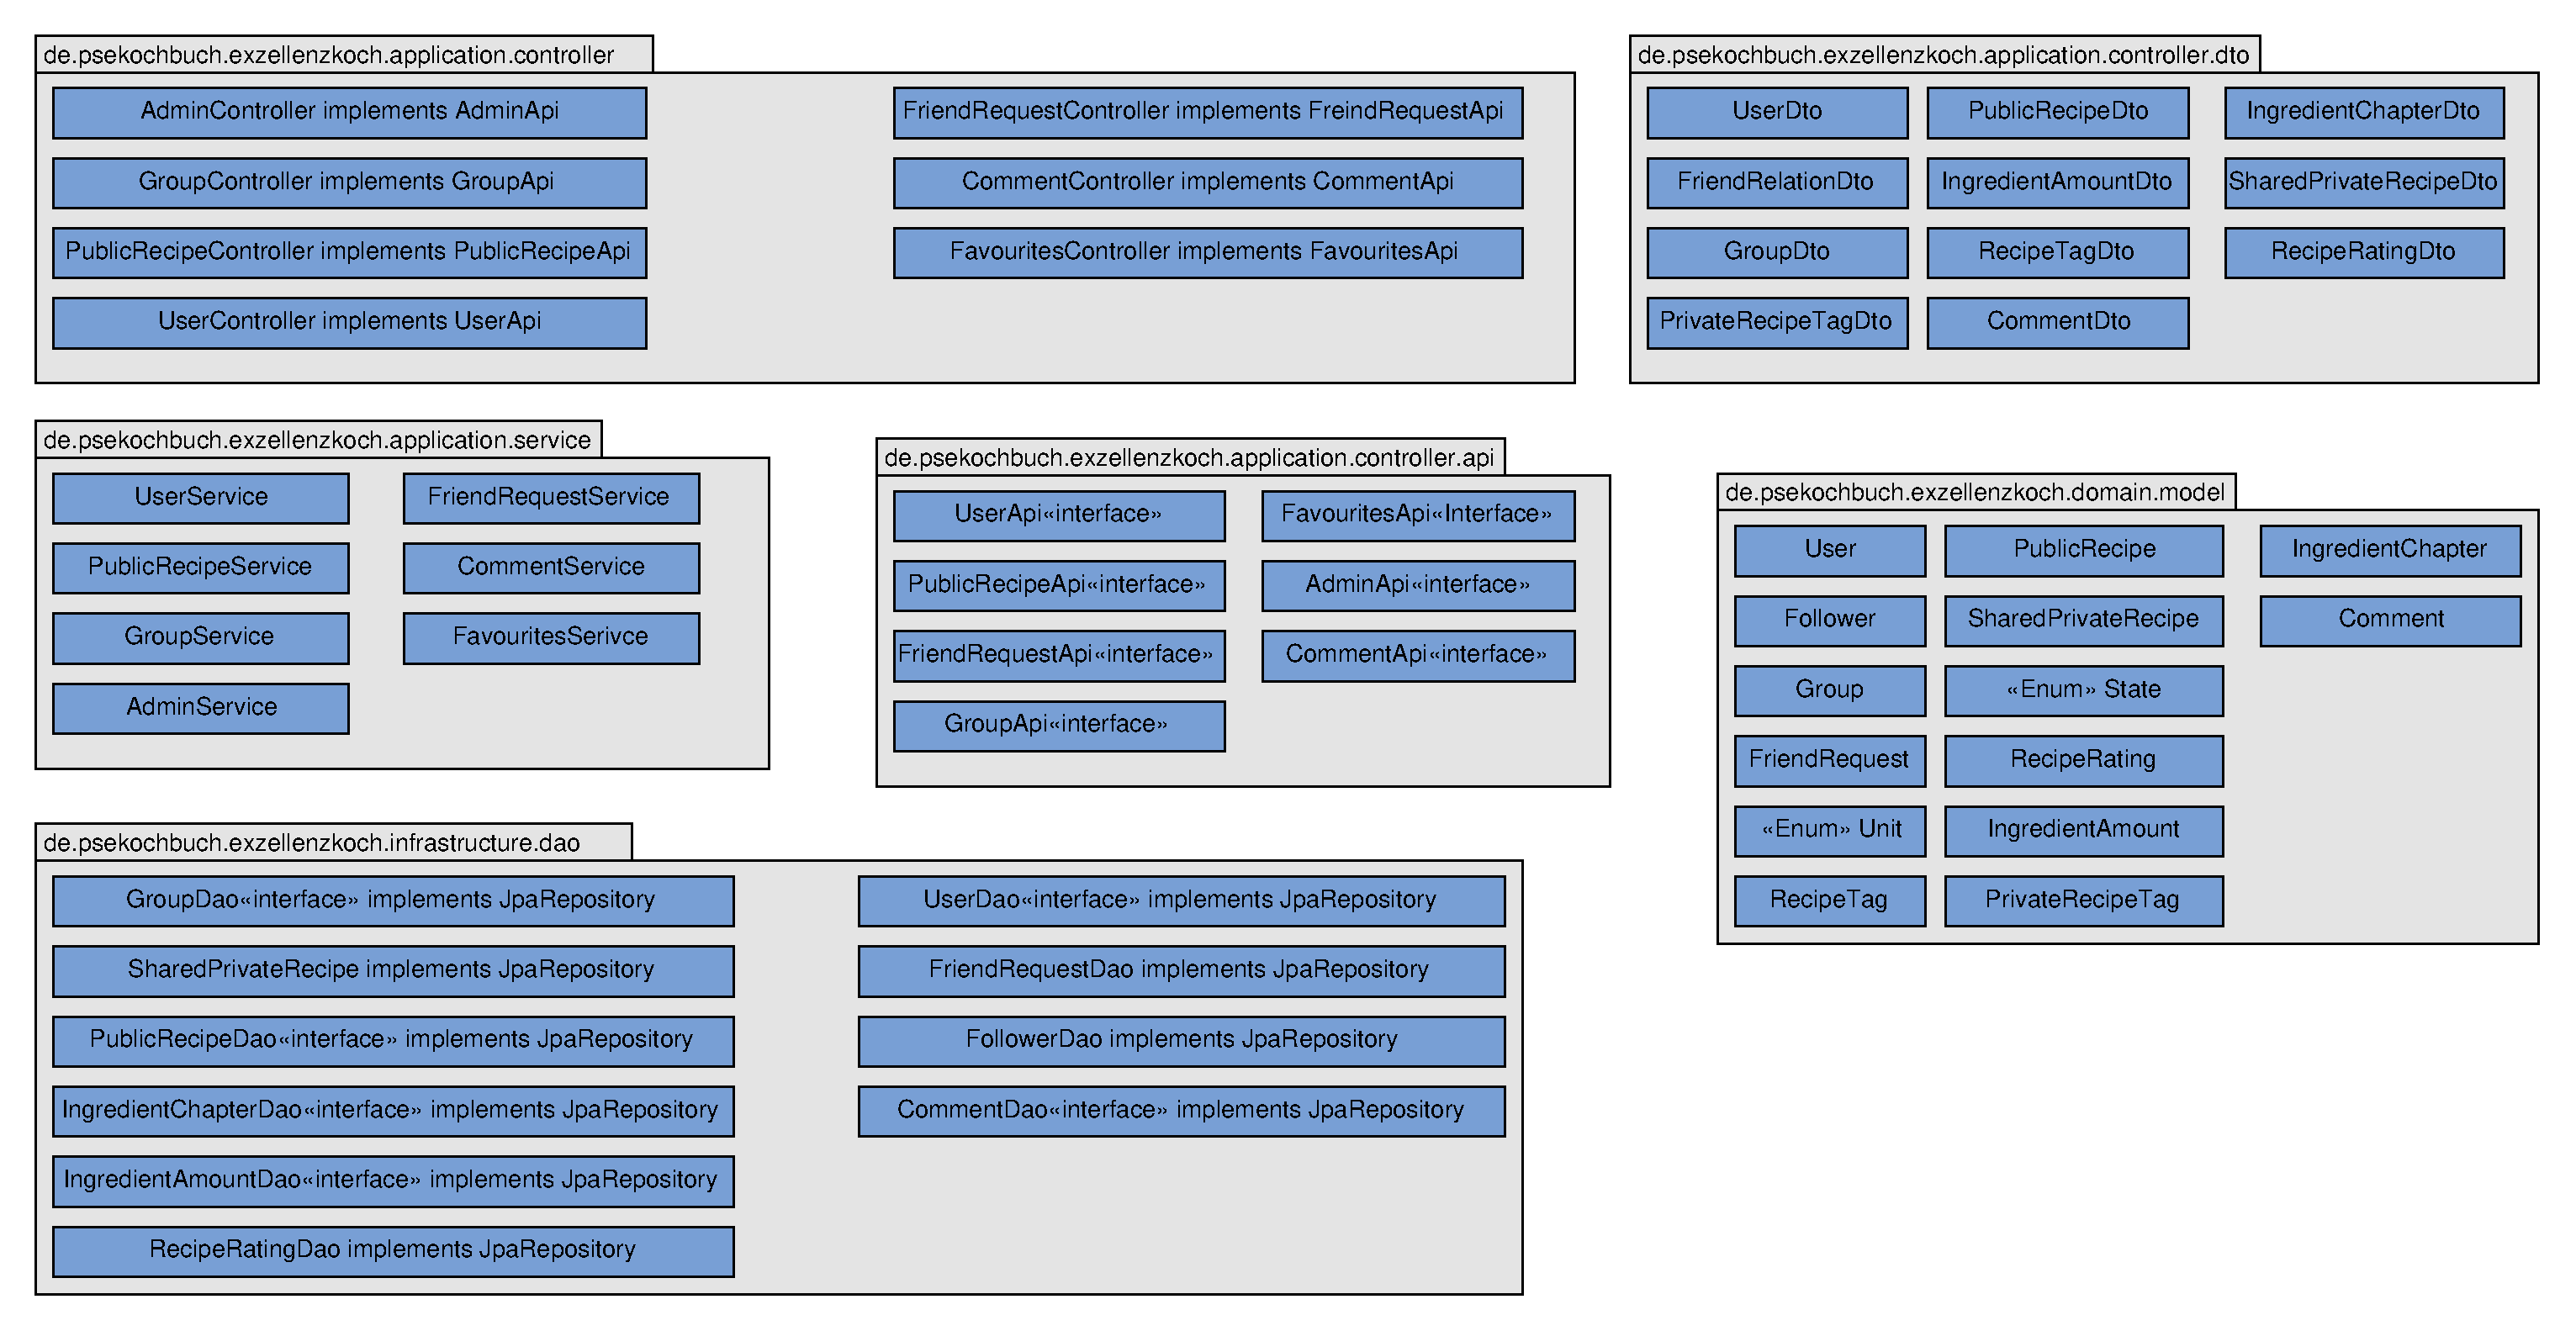
\includegraphics[width=\textwidth]{pics/PacketServerApi_and_Db.pdf}%
	\caption{Die Packages und Klassen für die ServerApi und die Anbindung an die Datenbank}%
	\label{serverapidb}
\end{figure}

\subsection{Konfiguration- und Ausführungspakete}
In der folgenden Abbildung \ref{serverconfig} werden alle Pakete und Klassen aufgelistet, welche für das Konfigurieren, Starten von dem Server und Authentifizieren von Nutzern zuständig sind.\\
Das Paket Security beinhaltet Klassen, die für die Authentifizierung von Nutzern, die den Dienst anfragen, verwendet werden. Die Klassen verwenden Spring Boot Security und Firebase. Das Paket exzellenzkoch enthält nur die Klasse ExzellenzkochApplication. Diese Klasse enthält die Main-Methode und startet den Dienst. Die Konfigurationsklassen befinden sich im Paket config. In WebSecurityConfig wird die Konfiguration der Spring Boot Security festgelegt und in der Klasse FirebaseConfig die Konfigurationen für die Firbaseverbindung. Im Paket exceptions befinden eine Exceptionenklasse, welche geworfen wird, wenn eine Element in der Datenbank nicht gefunden wird.

\begin{figure}[H]
	\centering
	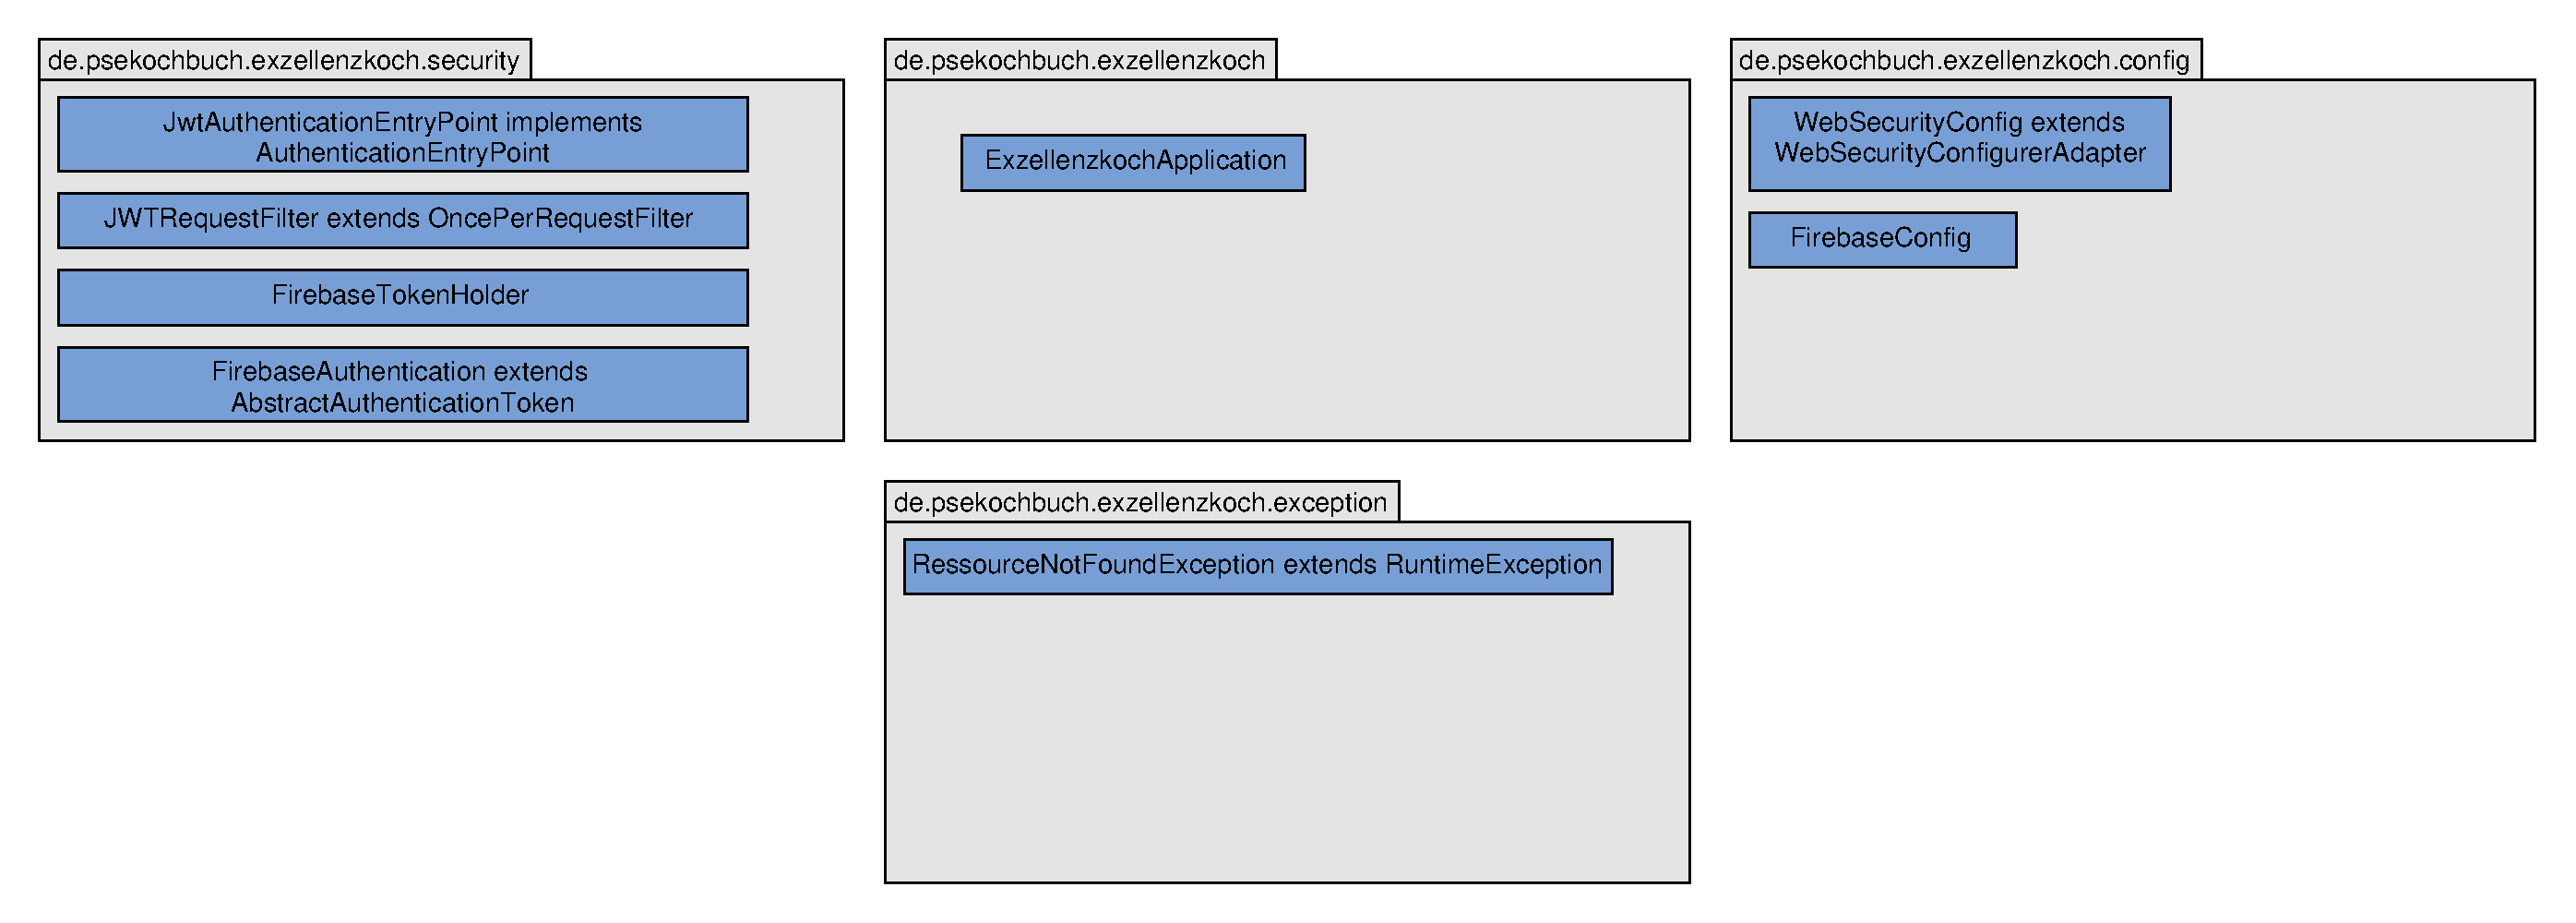
\includegraphics[width=\textwidth]{pics/PacketServerConfig.pdf}%
	\caption{Die Packages und Klassen für die Konfiguration und Ausführung des Servers und Authentifizierung von Nutzern}%
	\label{serverconfig}
\end{figure}

\subsection{Kommunikation zwischen Controllerpaket und Servicepaket}

\ref{kommContrServ} zeigt den Zugriff der Controller-Klassen auf die Service-Klassen. Jeder Controller greift auf seinen Service zu.

\begin{figure}[H]
	\centering
	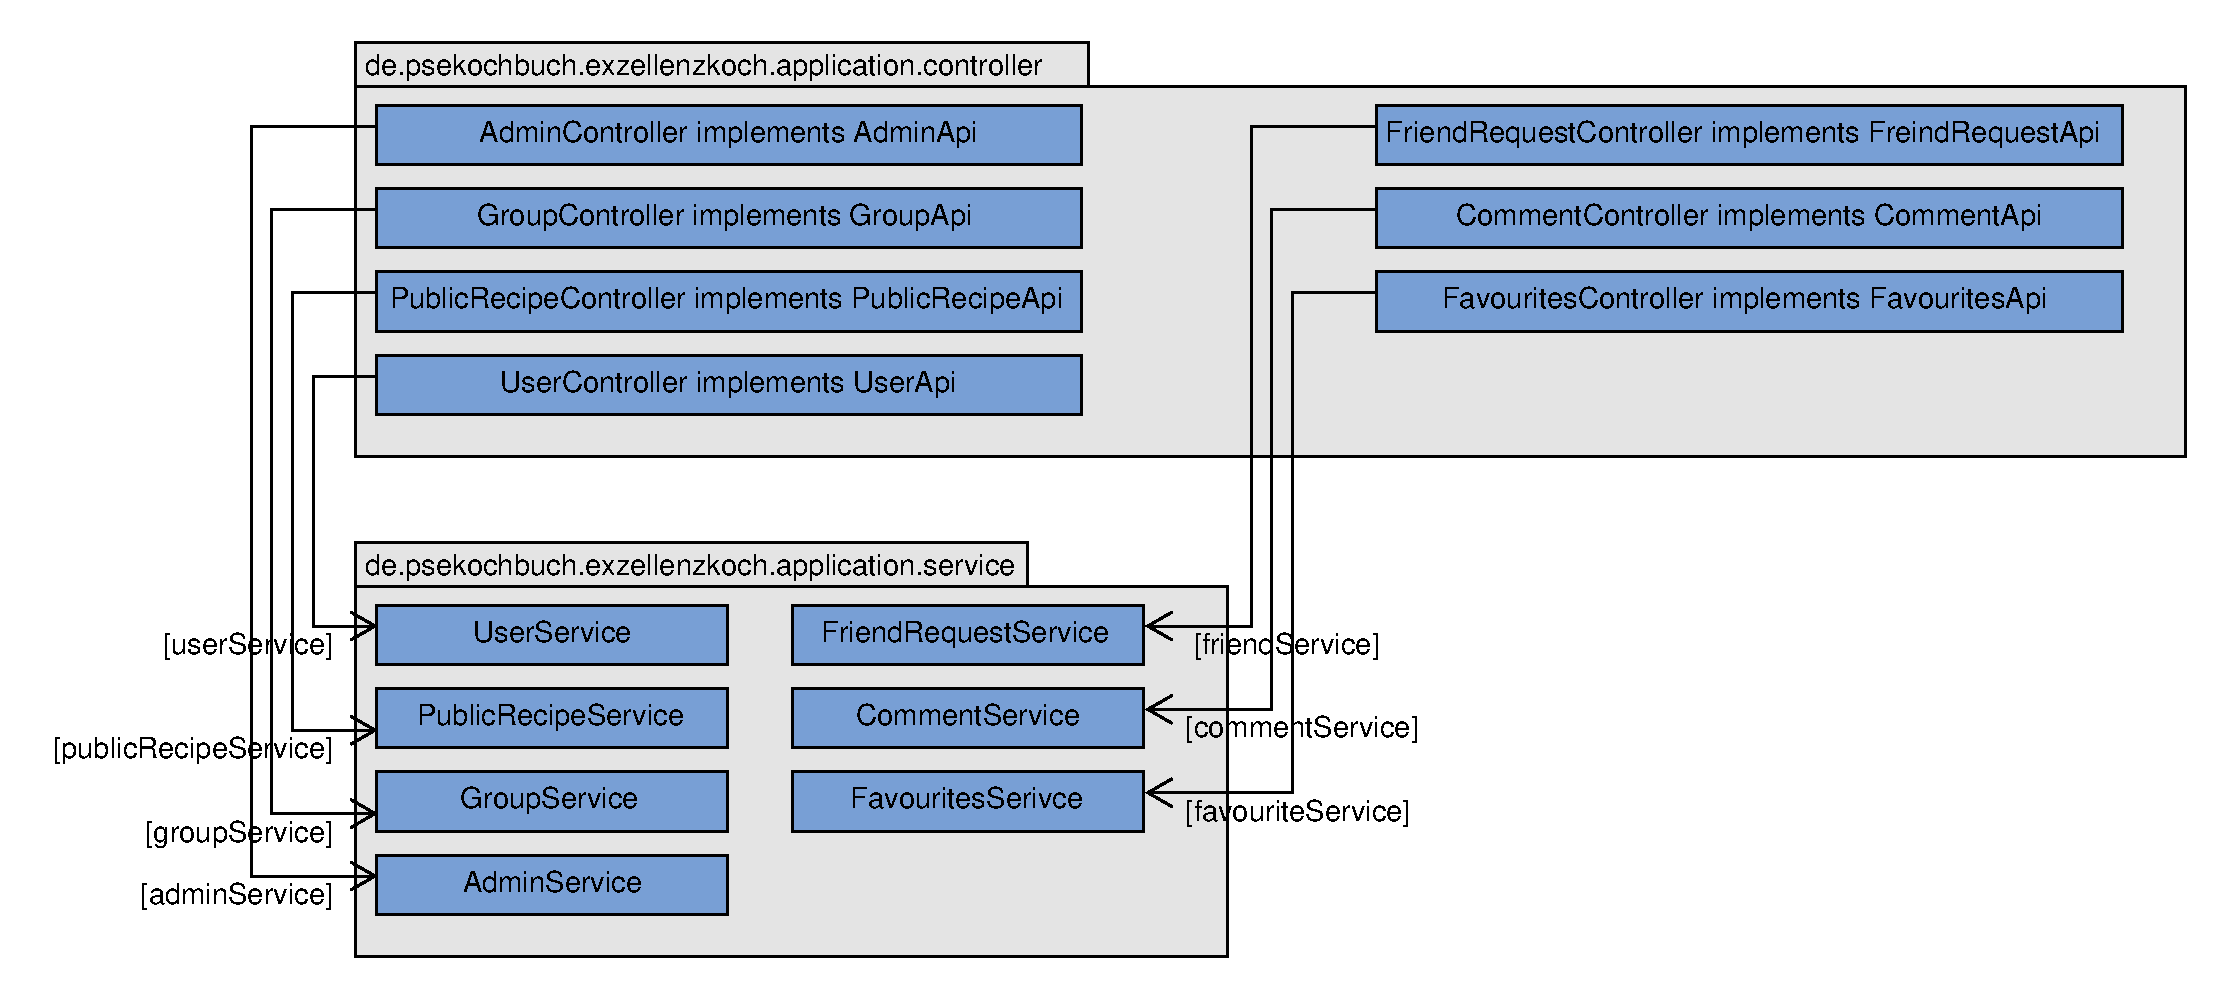
\includegraphics[width=\textwidth]{pics/KommunikationServerControllerService.pdf}%
	\caption{Die Packages und ihre Klassen und die Kommunikation zwischen Service und Controller}%
	\label{kommContrServ}
\end{figure}

\subsection{Kommunikation zwischen Servicepaket und Daopaket}

In \ref{kommServDao} wird der Zugriff der Service-Klassen auf die Dao-Klassen abgebildet. Ein Service kann auf verschiedene Dao zugreifen und ein Dao wird auch von verschiedenen Service-Klassen verwendet.

\begin{figure}[H]
	\centering
	\includegraphics[width=\textwidth]{pics/KommunikationServerServiceDao.pdf}%
	\caption{Die Packages und ihre Klassen und die Kommunikation zwischen Services und Dao}%
	\label{kommServDao}
\end{figure}



\chapter{Klassenbeschreibung Userinterface}

In diesem Kaptiel werden konkrete Attribute und Funktionalitäten der Klassen der App vorgestellt.

\section{View}

\subsection{Toolbar und Appmenü}

Das Userinterface der App besteht aus einer einzigen Activity ("`MainActivity"'), aus der heraus verschiedene Fragments aufgerufen werden können. Zu jedem Fragment gehört ein ViewModel.
In der MainActivity ist eine Toolbar definiert. In dieser Toolbar ist das Appmenü enthalten. Das Appmenü ist ein eigenes Fragment. Es wird über den Menübutton, der in der Toolbar liegt, aufgerufen und bietet über Buttons Zugriff zu verschiedenen ausgewählten Fragments.
Diese Fragments sind:
\begin{itemize}[nosep]
	\item RecipeListFragment: in Abb. \ref{menu} dargestellt durch Button: "`Meine Rezepte"'
	\item ShoppigListDisplayFragment: in Abb \ref{menu} dargestellt durch Button: "`Einkaufsliste"'
	\item FavouriteFragment: in Abb \ref{menu} dargestellt durch Button: "`Admin"'
	\item LoginFragment: in Abb \ref{menu} dargestellt durch Button: "`Login"'
	\item AdminFragment: in Abb \ref{menu} dargestellt durch Button: "`Admin"'
	\item FriendlistFragment (wenn \textbf{W14} implementiert ist): in Abb \ref{menu} dargestellt durch Button: "`Freunde"'
	\item FriendGroupFragment (wenn \textbf{W14} implementiert ist): in Abb \ref{menu} dargestellt durch Button: "`Gruppen"'
	\item Feed Fragment (wenn \textbf{W15} implementiert ist): in Abb \ref{menu} dargestellt durch Button: "`Feed"'
\end{itemize}

Implementiert: \textbf{F19, F25, F71}

\begin{figure}[H]
	\centering
	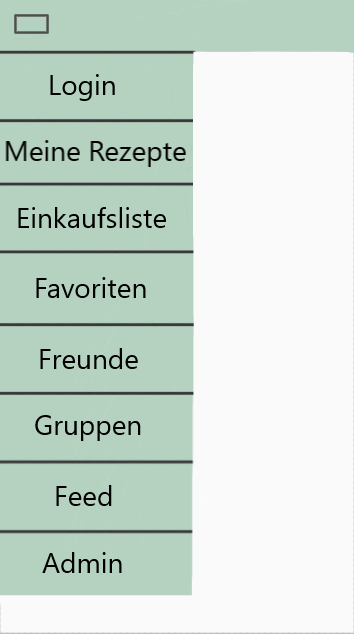
\includegraphics[width=0.7\textwidth]{pics/ToolbarMenu.png}%
	\caption{Toolbar mit angezeigtem Appmenü}%
	\label{menu}%
\end{figure}

Im Folgenden werden die einzelnen Fragments mitsamt ihren Inhalten beschrieben.

%Fragments
\subsection{CreateRecipeFragment}

\begin{figure}[H]
	\centering
	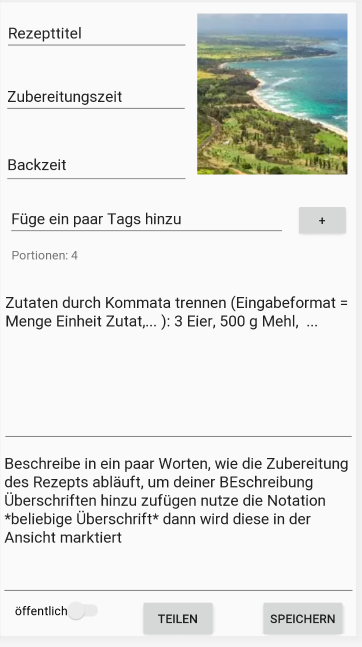
\includegraphics[width=0.7\textwidth]{pics/createRecipeFragment.png}%
	\caption{CreateRecipeFragment}%
	\label{view}%
\end{figure}
Implementiert: \textbf{F1, F2, F3, F4, F5, F6, F7, F8, F9, F10, F11, F13, F14, F15, F16, F20, F26, F32, F28, F29, F30, F31, F74, F75}
\begin{itemize}[nosep]
	\item 	Rezepttitel-EditText: Hier kann der Nutzer einen Titel für sein Rezept eingeben 
	\item 	Zubereitungszeit-EditText: Die Zeit, die zur Vorbereitung benötigt wird.
	\item 	Backzeit-EditText: Die Zeit, die das Gericht gebacken warten muss.
	
	\item 	Tagfeld-TextView: Hier kann der Nutzer Tags für sein Rezept hinzufügen. 
	
	\item Portionen-TextView: Das Portionen Feld
	\item PortionenAnzahl-EditText: Die Anzahl an Portionen, die man bei der Zubereitung des Rezepts bekommt. 
	\item Zutatenfeld-EditText: Alle Zutaten, die man zur Zubereitung des Gerichts braucht. Das Eingabeformat ist für jede Zutat "Menge Einheit Zutat", damit der Konvertierungsschritt zu einem öffentlich einsehbarem Rezept reibungslos abläuft.
	\item 	Zubereitung-Textfeld: Hier kann der Nutzer mit Text beschreiben, wie man das Rezept schrittweise zubereitet. Damit der Nutzer Überschriften in seiner Beschreibung hervorzuheben kann, gibt es die Möglichkeit die hervorzuhebenden Zeichen innerhalb zweier *-Symbole zu schreiben, wodurch beim Konvertieren zu einem öffentlichen Rezept diese Zeichen geparsed werden. Um andere Rezepte in seinem Text zu verlinken, kann der Nutzer den HTTP-Link eines Rezepts einfügen, um auf dieses Rezept verweisen. Diesem Link kann er ein Wort zuordnen, was statt des Links angezeigt wird.
	
	\item 	öffentlich-Switch: Falls der Nutzer sein Rezept veröffentlichen will kann er dies über den Schieberegler. Ist ein Rezept schon öffentlich und der Nutzer will dieses wieder als privat deklarieren ist das auch über diesen Regler machbar.
	
	\item 	Speichern-Button: Der Nutzer kann hierüber das Rezept in seiner Rezeptliste speichern. Falls der öffentlich-Schieberegler aktiviert ist, erfolgt die eine Vollständigkeitskontrolle und die Konvertierung.
	\item Teilen-Button: Der Nutzer hat die Möglichkeit hierüber das Rezept in andere Applikationen zu exportieren.
	\item Teilen-Button: Über den Speicher Button kann man das Rezept an externe Applikationen exportieren.
\end{itemize}


\subsection{RecipeListFragment}
\begin{figure}[H]
	\centering
	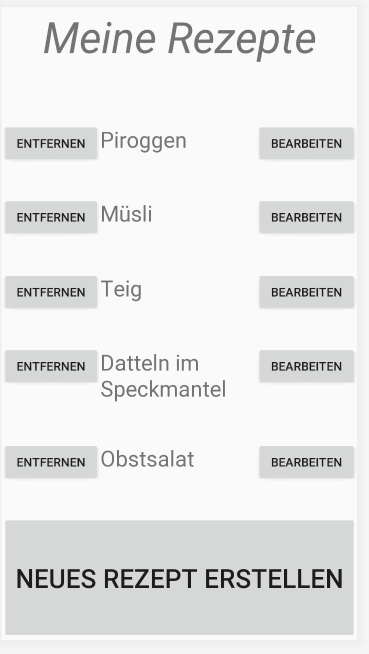
\includegraphics[width=0.7\textwidth]{pics/recipelistFragment.png}%
	\caption{RecipeListFragment}%
	\label{view}%
\end{figure}

Implements: \textbf{F17, F76, F77}

\begin{itemize}[nosep]
	\item header-TextView: Meine Rezepte Überschrift.
	\item  Rezeptliste mit je:
	\subitem	- Bearbeiten-Button: Hierüber kann der Nutzer sein Rezept bearbeiten.
	\subitem	- Rezeptname-TextView: Anzeige des Rezeptnamens.
	\subitem	- Entfernen-Button: Hierüber kann das jeweilige Rezept gelöscht werden
	\item 	Neues Rezept Erstellen-Button: Hierüber kann der Nutzer ein neues Rezept erstellen 
\end{itemize}



\subsection{AddEditCommentFragment}
\begin{figure}[H]
	\centering
	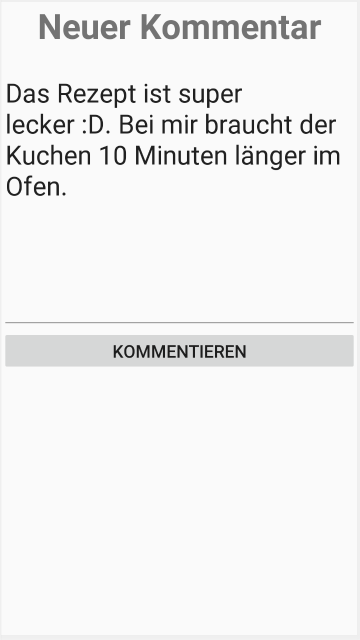
\includegraphics[width=0.7\textwidth]{pics/addeditCommentFragment.png}%
	\caption{AddEditCommentFragment}%
	\label{view}%
\end{figure}
Implementiert: \textbf{F37, F90}
\begin{itemize}[nosep]
	\item header-TextView: Hier wird "Neuer Kommentar angezeigt"
	\item 	Eingabe-Textfeld: Hier kann der Nutzer ein Kommentar in texlicher Form schreiben.
	\item 	Kommentieren-Button: veröffentlicht den Kommentar damit dieses in dem "RecipeDisplayFragment" gesehen werden kann
\end{itemize}

\subsection{DisplaySearchListFragment}
\begin{figure}[H]
	\centering
	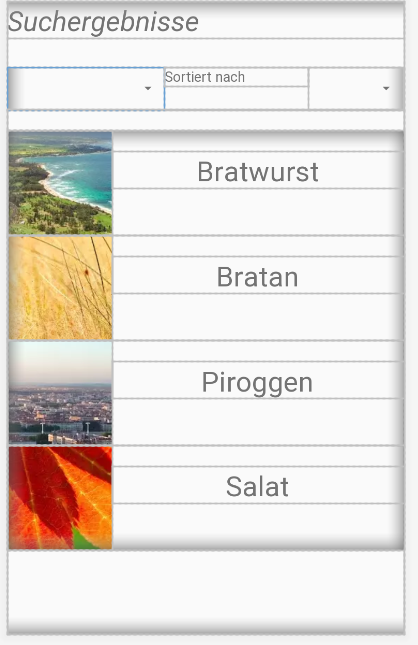
\includegraphics[width=0.7\textwidth]{pics/displaysearchlistFragment.png}%
	\caption{DisplaySearchListFragment}%
	\label{view}%
\end{figure}
Implementiert: \textbf{F53, F54, F55, F58, F88}
\begin{itemize}[nosep]
	\item 	Auswahlbox-Spinner: Der Nutzer hat die Auswahl zwischen absteigend und aufsteigend.
	\item 	Auswahlbox-Spinner: Der Nutzer hat die Auswahl zwischen verschiedenen Suchfiltern.
	\item 	Rezeptliste-ScrollView: Hier warten alle Suchergebnisse sortiert angezeigt. Der Nutzer kann die jeweiligen Rezepte auswählen, und wird dann auf das "RecipeDisplayFragment" weitergeleitet.
\end{itemize}

\subsection{UserSearchFragment}
\begin{figure}[H]
	\centering
	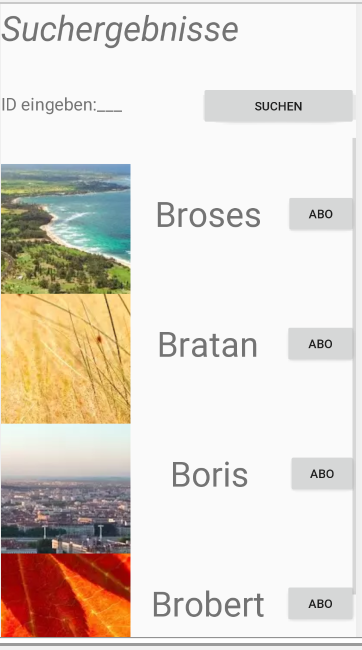
\includegraphics[width=0.7\textwidth]{pics/user_search_fragment.png}%
	\caption{UserSearchFragment}%
	\label{view}%
\end{figure}
Implementiert: \textbf{F48, F59, F60, F61, F62, F98}
\begin{itemize}[nosep]
	\item  header-TextView: "Suchergebnisse"
	\item 	ID-EditText: Hier kann die Nutzer-ID des gesuchten Nutzers eingetragen werden.
	\item Suchen-Button: Der Nutzer wählt den Suchen Button und bekommt eine Ergebnisliste von Nutzern angezeigt, die auf die eingetragene ID passen.
	\item Nutzerliste: Hier werden alle Suchergebnisse angezeigt.
	\item Abo-Button: Hierüber kann man einem Nutzer abonnieren.
\end{itemize}



\subsection{PublicRecipeSearchFragment}
\begin{figure}[H]
	\centering
	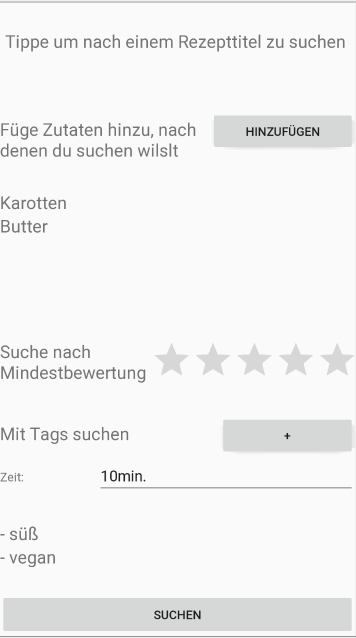
\includegraphics[width=0.7\textwidth]{pics/publicRecipeSearchFragment.png}%
	\caption{PublicRecipeSearchFragment}%
	\label{view}%
\end{figure}
Implementiert: \textbf{F51, F52, F56, F57}
\begin{itemize}[nosep]
\item	Titelsuche-Textfield: Der Nutzer kann hier einen Rezepttitel eingeben, nachdem gesucht werden soll
\item	Zutatenhinzufügen-Textfield \& Button: über das Textfeld kann der Nutzer eine Zutat eingeben und über den Button in eine Liste eintragen

\item	Zutatenliste-TextView: Hier werden alle eingegebenen Zutaten gespeichert, mit denen gesucht werden soll

\item Zeit-TextView: Zeit Anzeige
\item Zeitminuten-EditText: Minuten Eingabe
\item	Tag-suchen-Button: Hierüber kommt der Nutzer zur Suche mit Tags
\item Mindestbewertung: Textanzeige und Rating-Bar-Button
\item	Tag-Anzeige: Hier werden die Tags angezeigt, die zur Suche genutzt werden sollen 
\item	Suchen-Button: Wenn der Nutzer seine Suchoptionen eingegeben hat, kann er über den Button die Suche starten
\end{itemize}


\subsection{FeedFragment}
\begin{figure}[H]
	\centering
	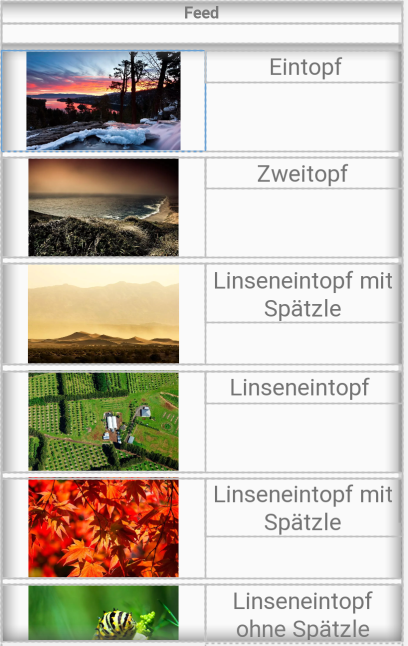
\includegraphics[width=0.7\textwidth]{pics/feedFragment.png}%
	\caption{FeedFragment}%
	\label{view}%
\end{figure}
Implementiert: \textbf{F70, F72}
\begin{itemize}[nosep]
	\item header-TextView: "Feed" Anzeige
	\item	RezeptListe: Hier werden alle Rezepte des Feeds angezeigt und können vom Nutzer ausgewählt werden. Dann kommt der Nutzer auf das jeweilige "RecipeDisplayFragment".
\end{itemize}
Der Feed zeigt die aktuellsten Rezepte an, die veröffentlicht wurden. Bei jedem neuen Laden des Feeds wird die Ansicht aktualisiert.

\subsection{ProfileDisplayFragment}
\begin{figure}[H]
	\centering
	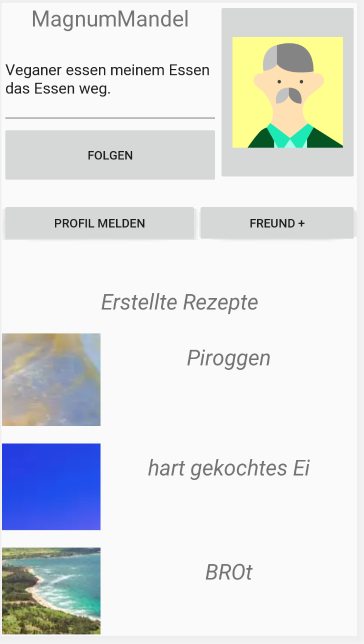
\includegraphics[width=0.7\textwidth]{pics/profilDistplayFragment.png}%
	\caption{ProfileDistplayFragment}%
	\label{view}%
\end{figure}
Implementiert: \textbf{F47, F63, F91}
\begin{itemize}[nosep]
	\item Namensfeld-TextView: Hier wird die Benutzer-ID angezeigt
	
	\item Folgen-Button:Hier kann man dem angezeigten Nutzer folgen.
	
	\item Beschreibung-TextView: Hier wird angezeigt, wie sich der Nutzer in ein paar wenigen Sätzen beschrieben hat. 
	
	\item Profilbild-ImageView: Der Benutzer kann ein Profilbild anzeigen lassen. Falls er dies nicht will, wird ein Standardbild angezeigt.
	
	\item Profilmelden-Button: falls ein Profil unangemessene Inhalte enthält, kann dieses hierdurch gemeldet werden, worauf es manuell von einem Admin geprüft wird.
	
	\item Freund+-Button: Nutzer können hierdurch anderen Nutzern eine Freundschaftsanfrage schicken
	
	\item Erstellte Rezepte-Liste: Hier werden alle öffentlich gestellten Rezepte des Nutzers angezeigt. Wenn man eins auswählt, kommt man direkt zum jeweiligen "RecipeDisplayFragment".
\end{itemize}

\subsection{ProfileEditFragment}
\begin{figure}[H]
	\centering
	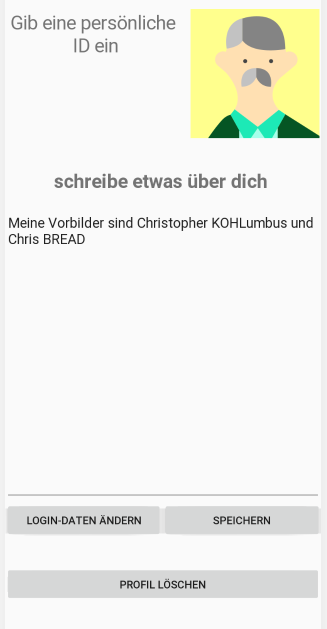
\includegraphics[width=0.7\textwidth]{pics/profileEditragment.png}%
	\caption{ProfileEditFragment}%
	\label{view}%
\end{figure}
Implementiert: \textbf{F41, F43, F44, F45, F46, F42}
\begin{itemize}[nosep]
	\item BenutzerID-EditView: Hier kann die Benutzer-ID eingetragen werden
	\item Profilbild-ImagView: Hier kann der Nutzer ein Profilbild hochladen und ändern.
	\item Beschreibung-Textfield: Hier kann sich der Nutzer in ein paar Worten selbst beschreiben. Dies ist auch in der öffentlichen Ansicht des Nutzerprofils sichtbar.
	\item Login-Daten-Ändern-Button: Falls der Nutzer seine Anmelde-Daten ändern möchte, kann er dies mit diesem Button machen
	\item Speichern-Button: der Nutzer speichert über diesen Button die Änderungen für sein Profil.
	\item löschen-Button: Hierüber entfernt der angemeldete Nutzer sein Profil, wodurch alle seine Daten, bis auf die privaten Rezepte, gelöscht werden.
\end{itemize}
Auf diesem Fragment kann der Nutzer alle öffentlich angezeigten Informationen ändern. Will er seine Daten zum Einloggen ändern erreicht er dies über den Login Daten ändern Button.

\subsection{RegistrationFragment}
\begin{figure}[H]
	\centering
	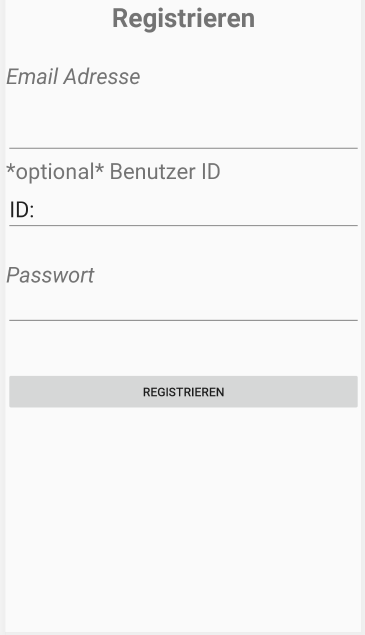
\includegraphics[width=0.7\textwidth]{pics/registrationFragment.png}%
	\caption{RegistrationFragment}%
	\label{view}%
\end{figure}
Implementiert: \textbf{F38, F39}
\begin{itemize}[nosep]
	\item header-TextView:"Registrieren"-Kopfzeile
	\item Email-Adresse-Textfield: Hier kann der Nutzer seine Email Adresse angeben
	\item Passwort-EditText:Hier kann der Nutzer sein Passwort angeben
	\item Benutzer ID -EditText: Hier kann der Nutzer eine Wunsch ID eintragen. Macht er dies nicht wird bei der Registrierung automatisch eine erstellt. 
	\item Registrieren-Button: Wenn der Nutzer seine Daten eingetragen hat, kann er über diesen Button die Registrierung abschließen
\end{itemize}
Bei der Registrierung hat der Nutzer drei Eingabefelder gegeben. Die Pflichtfelder für eine erfolgreiche Registrierung sind die Email-Adresse und  Passwort. Gibt der Nutzer diese gar nicht oder fehlerhaft an, wird der Prozess nicht weitergeführt. Des Weiteren kann der Nutzer eine BenutzerID für sich festlegen. Die Benutzer-ID und das Passwort können im Nachhinein noch geändert werden und sind nicht permanent. Die Email hingegen ist ab der erfolgreichen Registrierung nicht mehr änderbar.

\subsection{ChangePasswordFragment}
\begin{figure}[H]
	\centering
	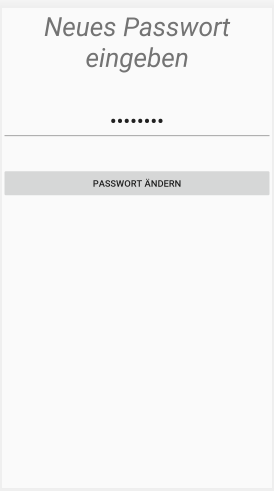
\includegraphics[width=0.7\textwidth]{pics/change_password_fragment.png}%
	\caption{ChangePasswordFragment}%
	\label{view}%
\end{figure}
Implementiert: \textbf{F40}
\begin{itemize}[nosep]
	\item Passwort-Textfield: Hier kann der angemeldete Nutzer sein neues Passwort eingeben.
	\item Passwort ändern - Button: Hierüber bestätigt der Nutzer sein neues Passwort
	
\end{itemize}
Da die Applikation die Account Funktionalität über Firebase verwaltet, werden die eingetragenen Daten direkt weitergegeben und so wenig wie möglich selbst gehalten. 


\subsection{LoginFragment}
\begin{figure}[H]
	\centering
	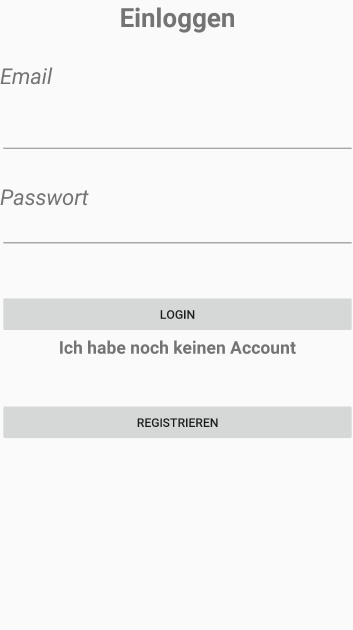
\includegraphics[width=0.7\textwidth]{pics/loginFragment.png}%
	\caption{LoginFragment}%
	\label{view}%
\end{figure}
Implementiert: \textbf{F50}
\begin{itemize}[nosep]
	\item Email-Textfield: Hier kannn der Nutzer seine Email angeben
	\item Passwort-Textfield:Hier kann der Nutzer sein Passwort angeben
	\item Login-Button: Wenn der Nutzer seine Daten eingetragen hat, kann er sich über diesen Button einloggen.
	\item Registrieren-Button: Falls der Nutzer noch kein Account hat, kann er auf den Registrieren Button klicken, um auf das RegistrationFragment geleitet zu werden.
\end{itemize}

\subsection{EditTagFragment}
\begin{figure}[H]
	\centering
	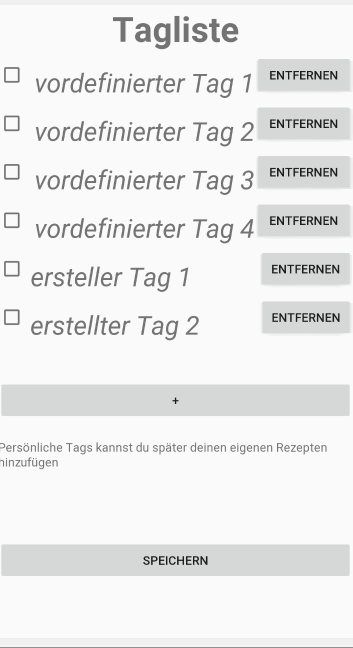
\includegraphics[width=0.7\textwidth]{pics/editTagFragment.png}%
	\caption{EditTagFragment}%
	\label{view}%
\end{figure}
Implementiert: \textbf{F73}
\begin{itemize}[nosep]
	\item Tag-Textfield: Hier kannn der Nutzer seine neuen Tags eingeben
	\item +-Button: Falls der Nutzer neue Eingabefelder braucht, kann er über den Button diese anfordern
	\item Speichern-Button: Wenn der Nutzer seine Tags eingetragen hat, kann er über den Speichern Button die Erstellung abschließen
\end{itemize}

\subsection{SearchWithTagsFragment}
\begin{figure}[H]
	\centering
	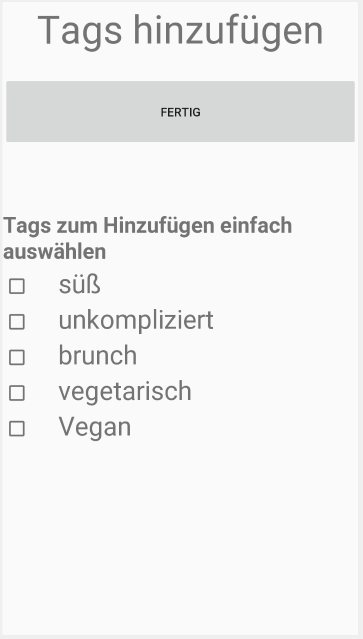
\includegraphics[width=0.7\textwidth]{pics/searchWithTagsFragment.png}%
	\caption{SearchWithTagsFragment}%
	\label{view}%
\end{figure}
\begin{itemize}[nosep]
	\item Tag-Auflistung: Hier werden alle vom User gesammelten Tags aufgelistet. Diese kann der Nutzer über eine Auswahlbox markieren.
	\item Fertig-Button: Wenn der Nutzer seine gewünschten Tags gesammelt hat, mit denen er suchen will, kann er über den Fertig-
	Button zurück zur Rezeptsuche gehen, wobei die Tags mitgenommen werden.

\end{itemize}

\subsection{AdminFragment}
\begin{figure}[H]
	\centering
	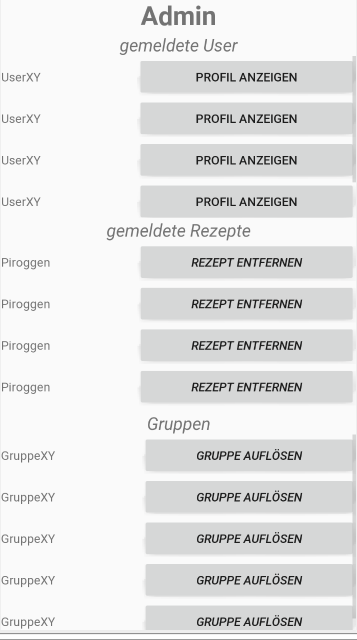
\includegraphics[width=0.7\textwidth]{pics/adminFragment.png}%
	\caption{AdminFragment}%
	\label{view}%
\end{figure}

\begin{itemize}[nosep]
	\item Nutzer-Auflistung: Hier sieht der Admin alle gemeldeten Nutzer. Er kann sich die Profile ansehen und einzelne nicht erlaubte Einträge (Bild, ID, Beschreibung) entfernen
	\item Rezept-Auflistung:Hier sieht der Admin eine Liste von allen gemeldeten Rezepten. er kann diese manuell überprüfen und direkt über den Button entfernen. 
	\item Gruppen-Auflistung: Hier sieht der Admin alle Gruppen, die gemeldet wurden. Falls ein Gruppenname nicht erlaubt ist, kann der Admin über den Button die Gruppe auflösen.
\end{itemize}
Der Admin hat über die Applikation die Möglichkeit Rezepte und Gruppen direkt zu entfernen. Falls ein Nutzer ein unpassenden Namen, Beschreibung, oder Bild hat muss sich der Admin dieses manuell ansehen und entscheiden, ob nur das jeweilige Feld aus der Datenbank austrägt, oder den Nutzer komplett entfernt.

\subsection{ShoppingListDisplayFragment}
\begin{figure}[H]
	\centering
	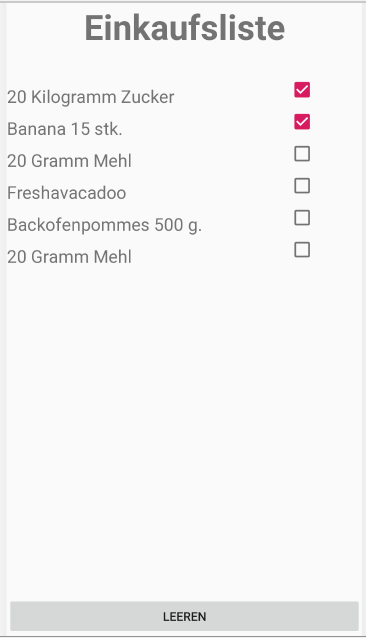
\includegraphics[width=0.7\textwidth]{pics/shoppingListdisplayFragment.png}%
	\caption{ShoppingListDisplayFragment}%
	\label{view}%
\end{figure}
Implementiert: \textbf{F21, F24}
\begin{itemize}[nosep]
	\item Zutaten-Auflistung: Hier werden alle Zutaten, die der Nutzer seiner Einkaufliste hinzugefügt an angezeigt. Diese kann er über eine Checkbox abhaken. 
	\item leeren-Button: Falls die Liste nicht mehr benötigt wird, kann der Nutzer diese über den Button leeren.
\end{itemize}

\subsection{FriendListFragment}
\begin{figure}[H]
	\centering
	
	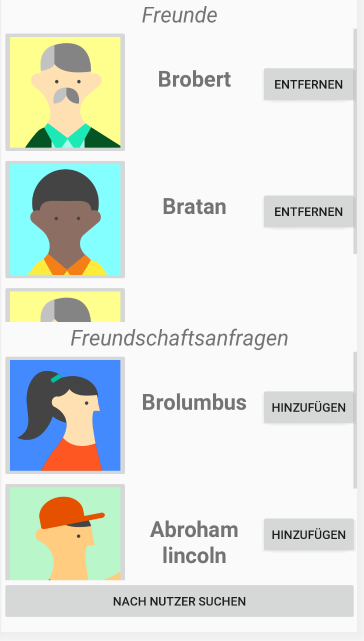
\includegraphics[width=0.7\textwidth]{pics/friendListFragment.png}%
	\caption{FriendListFragment}%
	\label{view}%
\end{figure}
Implementiert: \textbf{F64, F65, F66, F92}
\begin{itemize}[nosep]
	\item Freundesauflistung:Hier werden alle schon bestätigten Freunde des Nutzers angezeigt. Wenn man eine Person anklickt, kommt man zur jeweiligen Profilansicht.  
	
	\item Freundschaftsanfragen:Hier werden alle Nutzer angezeigt, die eine Freundschaftsanfrage gesendet haben. Wenn man eine Person anklickt, kommt man zur jeweiligen Profilansicht. 
	\item Suchen-Button: Hierüber kommt man zu einer Ansicht, die eine Benutzersuche bereitstellt
	\item Entfernen-Button: Der Freund wird aus der Freundesliste entfernt
	\item Hinzufügen-Button: Der Freund wird der Freundesliste hinzugefügt
\end{itemize}

\subsection{GroupMemberListFragment}
\begin{figure}[H]
	\centering
	
	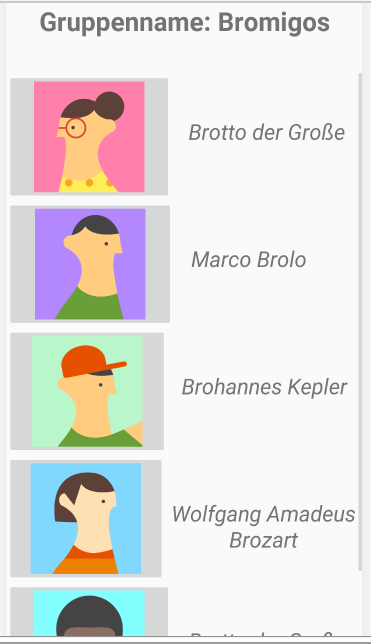
\includegraphics[width=0.7\textwidth]{pics/groupMemberListFragment.png}%
	\caption{GroupMemberListFragment}%
	\label{view}%
\end{figure}


\begin{itemize}[nosep]
	\item Gruppenname-TextView: Name Der Gruppe 
	\item Gruppenmitglieder-Auflistung:Hier werden alle Mitglieder der Gruppe aufgelistet. Wenn man sie auswählt, kommt man zur jeweiligen Profilansicht.
\end{itemize}


\subsection{CreateGroupFragment}
\begin{figure}[H]
	\centering
	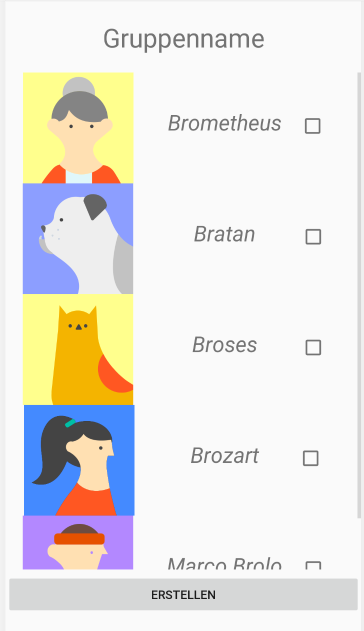
\includegraphics[width=0.7\textwidth]{pics/createGroupFragment.png}%
	\caption{CreateGroupFragment}%
	\label{view}%
\end{figure}
Implementiert: \textbf{F67, F68, F93, F94}
Wir müssen auch sorgen, das im nachinein Mitglieder hinzugefügt werden können, dafür kann ja dieses Fragment recycled werden
\begin{itemize}[nosep]
	\item Gruppenname-TextView: Gruppenname wird angezeigt
	\item Freunde-Auflistung:Hier werden alle Freunde des Nutzers aufgelistet. Über die Checkbox auf der rechten Seite kann man einen Gruppe beim Erstellen der Gruppe hinzufügen. Drückt man auf einen Nutzer, kommt man nicht auf die jeweilige Profilseite.
\end{itemize}

\subsection{FriendGroupFragment}
\begin{figure}[H]
	\centering
	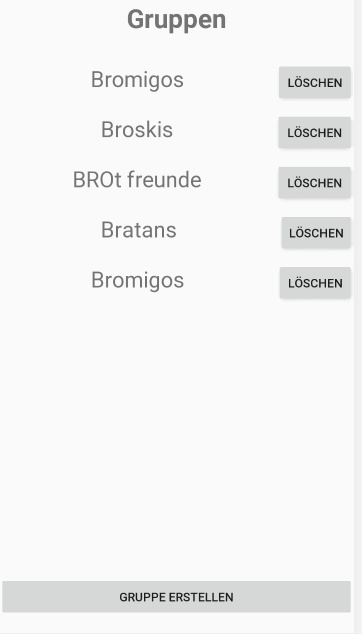
\includegraphics[width=0.7\textwidth]{pics/friendGroupFragment.png}%
	\caption{FriendGroupFragment}%
	\label{view}%
\end{figure}
Implementiert: \textbf{F68, F95}
\begin{itemize}[nosep]
	\item Gruppen-Auflistung: Hier werden alle Gruppen, in denen der Nutzer Mitglied ist, aufgelistet. 
	\item Löschen-Button
	\subitem - Falls er der Admin ist, wird die Gruppe komplett entfernt
	\subitem - Falls er nicht der Admin ist, entfernt er nur sich aus der Gruppe
	\item Gruppe-erstellen-Button: Hierüber kommt der Nutzer auf die Gruppe-Erstellen Ansicht.
\end{itemize}

\subsection{GroupFragment}
\begin{figure}[H]
	\centering
	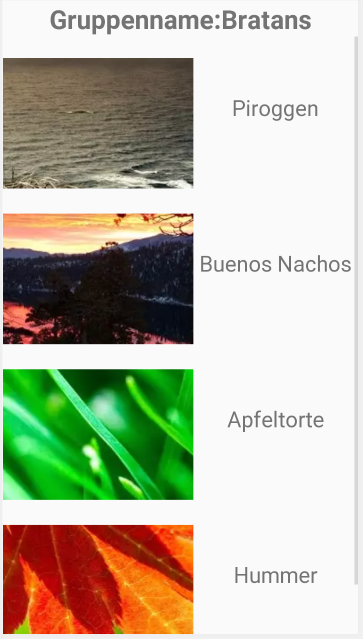
\includegraphics[width=0.7\textwidth]{pics/groupFragment.png}%
	\caption{GroupFragment}%
	\label{view}%
\end{figure}
Implementiert: \textbf{F69}
\begin{itemize}[nosep]
	\item Gruppenname: Hier wird der Gruppenname angezeigt und wenn man darauf klickt, kommt man auf die Gruppenmitglieder Ansicht
	\item Rezept-Auflistung: Hier werden alle geteilten Rezepte aufgelistet. Wenn man diese anklickt, kommt man auf die Rezept bearbeiten Ansicht. Da man private Rezepte in Gruppen teilen kann, können diese unvollständig sein. Daher kann man diese nur in der bearbeiten Ansicht anschauen.
\end{itemize}

\subsection{RecipeDisplayFragment}
\begin{figure}[H]
	\centering
	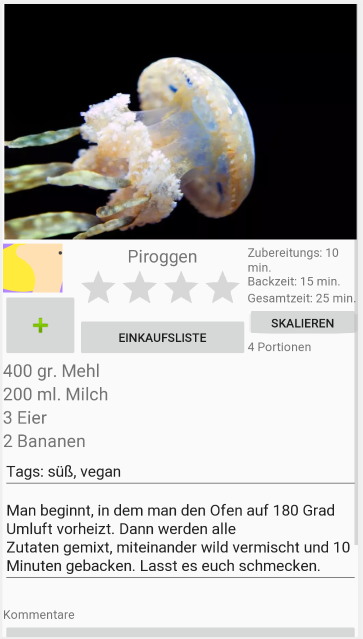
\includegraphics[width=0.7\textwidth]{pics/recipeDisplayFragment.png}%
	\newline
    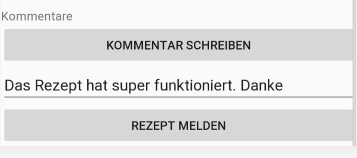
\includegraphics[width=0.7\textwidth]{pics/recipeDisplayFragmentzwei.png}%
	\caption{RecipeDisplayFragment}%
	\label{view}%
\end{figure}
Implementiert: \textbf{F18, F22, F23, F33, F34,F35, F36}
\begin{itemize}[nosep]
	\item Rezeptbild: Hier wird das Rezeptbild angezeigt
	\item Rezepttitel: Der Name des Rezepts
	\item Bewertungsfeld: Hier kann jeder angemeldete Nutzer eine Bewertung für das Rezept angeben
	\subitem Falls das Rezept schon vom Nutzer bewertet wurde, wird diese Bewertung angezeigt
	\item Zubereitungszeit: Hier steht die Zeit, die für die Zubereitung benötigt wird
	\item Backzeit: Hier steht die Zeit, die das Gericht gebacken werden muss
	\item Gesamtzeit: Diese ergibt aus der Zubereitungs- und der Backzeit
	\item Einkaufsliste-Button: Hierüber kann der Nutzer die Zutaten in seine Einkaufsliste eintragen. Daraufhin kommt er auch in die Einkaufslisten Ansicht
	\item skalieren-Button: Wenn der Nutzer eine neue Menge eingibt, werden die Portionen umgerechnet.
	\item Profilbild: Hier wird das Profilbild des Rezepterstellers angezeigt. Wenn man dieses anklickt, kommt man auf die Profilansicht des Erstellers.
	\item Hinzufügen-Button: Wenn man diesen anklickt, wird das Rezept in der Favoritenliste hinzugefügt
	\item Zutaten-Liste: Hier werden alle für das Rezept benötigten Zutaten aufgelistet
	\item Tag-Liste: Hier werden alle von dem Autor eingetragenen Tags angezeigt
	\item Beschreibung: Hier steht die Zubereitungsbeschreibung für das Rezept
	\item Kommentar schreiben - Button: Hier kann ein angemeldeter Nutzer ein Kommentar zu dem jeweiligen Rezept verfassen. Hierüber wird man auf das AddEditCommentFragment weitergeleitet. 
	Klick man auf ein Kommentar, das von einem selbst ist, wird man auf das AddEditCommentFragment weitergeleitet. 
	\item Kommentarliste: Hier werden alle zu dem Rezept schon verfassten Kommentare aufgelistet.
	\item Melden-Button: Hierüber kann das Rezept gemeldet werden. Daraufhin erscheint das Rezept in der Liste des Admins, der dieses dann manuell überprüfen kann. 
	
\end{itemize}

\subsection{FavouriteFragment}
\begin{figure}[H]
	\centering
	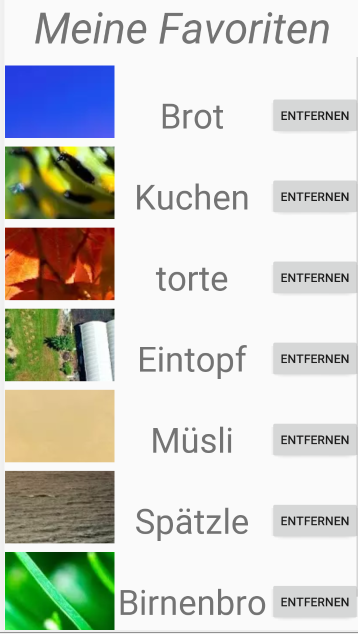
\includegraphics[width=0.7\textwidth]{pics/favouriteFragment.png}%
	\caption{FavouriteFragment}%
	\label{view}%
\end{figure}


\begin{itemize}[nosep]
	\item Rezeptliste: Hier werden alle favorisierten Rezepte angezeigt. Diese kann der Nutzer einzeln aus der Favoritenliste entfernen. Wenn auf ein Rezept geklickt wird, kommt man auf die jeweilige Rezeptansicht des Rezepts.
	\item entfernen-Button: Das Rezept wird gelöscht
\end{itemize}

%ViewModels
\newpage
\section{ViewModel}
Im Folgenden werden die den Fragments zugehörigen ViewModel-Klassen beschrieben.
Vorweg sei gesagt, dass alle ViewModels in der onCreate()-Methode der Main-Activity eingebunden werden müssen.
Jedes einzelne ViewModel wird außerdem in dem ihm zugehörigen Fragment instanziiert. Somit wird beim allerersten Aufruf des Fragments sein ViewModel erstellt, sodass dieses Daten für das Fragment bereitstellen kann.
Da Die Viewmodel an einigen Stellen einen redundanten Aufbau besitzen, werden die wichtigen Eigenheiten des ViewModels in der folgenden Beschreibung hervorgehoben. Ist ein Repository eingezeichnet, so sind die darin  beschriebenen Methoden aus Übersichtsgründen nur auf das jeweilige ViewModel abgestimmt. Im Entwurf wird es dennoch nur eine Klasse geben, das alle vorkommenden Methoden der ViewModel beinhaltet. Der Ablauf ist jeweils immer gleich, dass ein Fragment sein zugehöriges ViewModel erstellt, worüber der Zugriff auf das Repository stattfindet. Damit ist die Oberfläche der Applikation sauber von der Datenquelle getrennt. Die Relation zwischen dem jeweiligen ViewModel und dem Fragment ist über ein Oberserver Pattern beschrieben. Exemplarisch ist das im DisplaySearListViewModel näher erläutert. Dieses Obersever-Pattern soll für die weiteren ViewModel implizit angenommen werden, da es aus Redundanzgründen und der Übersichtlichkeit nicht modelliert wurde. Ähnlich redundant ist der Aufbau der Fragmente, der prinzipiell den Klassen entspricht, wie oben beschrieben  (Siehe Kapitel 5.1). Daher wurden die Fragmente nur skizzenhaft modelliert und nur eingefügt, wo es der Übersicht hilft.

\subsection{DisplaySearchListViewModel}
\begin{figure}[H]
	\centering
	\includegraphics[width=0.7\textwidth]{pics/viewModel/Display_Search_List_ViewModel.pdf}%
	\caption{DisplaySearchList}%
	\label{viewModel}%
\end{figure}

\begin{itemize}
	\item \textcolor{blue}{DisplaySearchListViewModel(title:String, ingredients:List<String>, rating:int, tags:List<String>, time:int)}\textcolor{cyan}{:constructor} Im Konstruktor werden alle Suchparameter übergeben \textbf{F53, F54, F56}
	
	\item \textcolor{blue}{sortRecipes()}\textcolor{cyan}{:void} Diese Methode sortiert die aufgelisteten Rezepte nach dem gewünschten Kriterium. Der Nutzer kann das Kriterium in einer Ausklappbaren Leisten im Fragment auswählen. Diese Kriterien beinhalten beispielsweise: Datum, Bewertung,... \textbf{F55, F58} 
	
	\item \textcolor{blue}{getRecipes()} \textcolor{cyan}{:List<PublicRecipe>} Diese Methode lädt die jeweiligen Rezepte, die auf die Eingaben des "PublicRecipeSearchFragment" passen, aus dem Repository.
\end{itemize}

\subsubsection{Observer Entwurfsmuster}
Observer
Durch den Observer ist es möglich eine saubere Kapselung der Schichten in nur eine Richtung zu halten. Die View Schicht kennt die ViewModel schicht, jedoch nicht andersherum. Um trotzdem aktuell zu bleiben, nutzt man das Oberserver Pattern. Die ViewModel Schicht hält die View Schicht nicht als Assoziation, sondern wird automatisch bei einer Änderung benachrichtigt, dass sich was geändert hat. Damit gehört es zu den Verhaltensmustern und dient der Weitergabe von Änderungen an einem Objekt an von diesem Objekt abhängige Strukturen.




\subsection{CreateRecipeViewModel}
\begin{figure}[H]
	\centering
	\includegraphics[width=0.7\textwidth]{pics/viewModel/Create_Recipe_ViewModel.pdf}%
	\caption{CreateRecipeViewModel}%
	\label{viewModel}%
\end{figure}

\begin{itemize}
	\item \textcolor{blue}{CreateRecipeViewModel(privateRec:PrivateRecipe)}\textcolor{cyan}{:constructor} Wenn ein bestehendes Rezept bearbeited werden soll, wird dieses im Konstruktor übergeben und sonst ein null Pointer \textbf{F15}

	\item \textcolor{blue}{addTags()}\textcolor{cyan}{:void} öffnet das  SearchWithTagsCreateRecipeFragment 
	
	\item \textcolor{blue}{setContent(title:String, preppingtime:Int, cookingtime:Int, servings,ingredients:List<String>, description:String, idPublic:String)}\textcolor{cyan}{:void} schreibt die bisher eingetragenen LiveData-Attribute (!=null) in das Rezept \textbf{F2, F3, F4, F5, F6, F7, F8, F9, F10}
	
	\item \textcolor{blue}{addToRepository(rec:PrivateRecipe}\textcolor{cyan}{:void} ruft erst setContent(...) auf und gibt dann das privateRecipe an das Repository zum Speichern in der SQLite DB
	
	\item \textcolor{blue}{parse(rec:PrivateRecipe)} \textcolor{cyan}{:PublicRecipe} wandelt das PrivateRecipe rec in ein PublicRecipe um. Dazu prüft die Methode alle Attribute des PrivateRecipe. Außerdem werden die HTTP-Links aus der Zubereitungsbeschreibung geprüft. Ist ein Link nicht gültig, wird der Nutzer mithilfe eines Alert-Dialogs gewarnt \textbf{F32}
	
	\item \textcolor{blue}{save()}\textcolor{cyan}{:void} unterscheidet, ob isPublic={true,false}.
	true: rufe parse() mit privateRec als Parameter auf 
	und schicke dann das Resultat ins Repository
	zum Speichern auf dem Server
	false: speichert Rezept nur lokal \textbf{F1, F11, F14}
	
	\item \textcolor{blue}{addToRepository(parse(privateRec))}\textcolor{cyan}{:void}
	false: rufe addToRepository(privateRecipe) auf und
	lasse somit das privateRec vom Repository in der 
	SQLite DB speichern. \textbf{F13, F16}
	
	
	
\end{itemize}


\subsection{RecipeListViewModel}
\begin{figure}[H]
	\centering
	\includegraphics[width=0.7\textwidth]{pics/viewModel/Recipe_List_ViewModel.pdf}%
	\caption{RecipeListViewModel}%
	\label{viewModel}%
\end{figure}
\begin{itemize}
	\item \textcolor{blue}{getPrivateRecipes()}\textcolor{cyan}{:List<PrivateRecipe>}
	alle privaten Rezepte werden geladen.
	\item  \textcolor{blue}{deletePrivateRecipe(id:String)}\textcolor{cyan}{:void}
	löscht ein privates Rezept. Falls dieses öffentlich ist, wird dieses auch vom Server entfernt \textbf{F17}
	\item \textcolor{blue}{editPrivateRecipe(recipe:PrivateRecipe)}\textcolor{cyan}{:void}Diese Methode löst einen Fragment wechsel aus, wobei das ausgewählte Rezept in das "CreateRecipeFragment" übergeben wird
	\item \textcolor{blue}{createnewRecipe()}\textcolor{cyan}{:void}
	Diese Methode löst einen Fragmentwechel aus, wobei auf das "CreateRecipeFragment" mit unausgefülltem Template gewechselt wird
\end{itemize}


\subsection{AddEditCommentViewModel}
\begin{figure}[H]
	\centering
	\includegraphics[width=0.7\textwidth]{pics/viewModel/AddEdit_Comment_ViewModel.pdf}%
	\caption{AddEditCommentViewModel}%
	\label{viewModel}%
\end{figure}
\begin{itemize}
	\item \textcolor{blue}{AddEditCommentViewModel(recipeId:int, commentId:int)} \textcolor{cyan}{:construct} Wenn ein Kommentar bearbeitet werden soll, wird die commentId hier übergeben
	
	\item \textcolor{blue}{addCommentToRecipe(...)} \textcolor{cyan}{:void}
	Ordnet dem Rezept über das Repository ein neues Kommentar hinzu, 
	falls die commentID noch nicht existiert. Falls die
	schon existiert, wird das bisherige ersetzt.
	
	\item \textcolor{blue}{loadComment(id:int)}\textcolor{cyan}{:Comment} 
	fragt über das Repository den Server an, ob ein Kommentar mit der 
	gegebenen ID existiert.Falls ja wird dieses zurückgegeben.
	
\end{itemize}
Der Nutzer ist hier, um ein Kommentar zu einem Rezept zu schreiben. Falls er ein schon bestehendes Kommentar ändern will, wird dieses schon in dem Textfeld angezeigt. Will der Nutzer ein neues Kommentar verfassen ist das Textfeld leer. Falls der Nutzer ein leeres Textfeld speichern will, kehrt der Nutzer auf das "RecipeDisplayFragment" zurück, ohne dass ein Kommentar hinzugefügt wird. 





\subsection{UserSearchViewModel}
\begin{figure}[H]
	\centering
	\includegraphics[width=0.7\textwidth]{pics/viewModel/User_Search_ViewModel.pdf}%
	\caption{UserSearchViewModel}%
	\label{viewModel}%
\end{figure}
\begin{itemize}
	\item \textcolor{blue}{followUser(userID:String)}\textcolor{cyan}{:void}  fügt den übergebenen User in die Abonnementliste des Senders ein. \textbf{F48}
	
	\item \textcolor{blue}{getUsers(userID:String)}\textcolor{cyan}{:List<User>} gibt die User, deren ID mit userID beginnt, zurück. \textbf{F59, F60, F61}
\end{itemize}
Jeder Nutzer kann über die Sucheingabe die Benutzer-ID eines registrierten Nutzers eingeben. Klickt er dann auf "`suchen"', so werden in einer Liste alle passenden Ergebnisse angezeigt. Die Benutzer-ID muss eindeutig sein. Trotzdem ergibt es Sinn, auch verschiedene Suchergebnisse anzuzeigen, da der Suchende eventuell nur ein Präfix der eigentlichen ID kennt, oder eingegeben hat. Demnach sollen alle Nutzer angezeigt werden, die auch diesen Präfix beinhalten. 
Im Pflichtenheft wurde beschrieben, dass die Benutzersuche durch mehrere Suchfilter eingeschränkt werden kann. Da die Architektur der Applikation in ihrer Grundfunktion jedoch nicht darauf ausgelegt ist, weil vorerst die ID der primäre eindeutige Bezeichner für einen angemeldeten Nutzer ist, wird diese Funktion nicht implementiert.

\subsection{PublicRecipeSearchViewModel}
\begin{figure}[H]
	\centering
	\includegraphics[width=0.7\textwidth]{pics/viewModel/Public_Recipe_Search_VieModel.pdf}%
	\caption{PublicRecipeSearchViewModel}%
	\label{viewModel}%
\end{figure}
\begin{itemize}
	\item  \textcolor{blue}{addIngredientToList()}\textcolor{cyan}{:void}
	Fügt der Suchliste Zutaten hinzu.
	\item  \textcolor{blue}{addTags()}\textcolor{cyan}{:void} öffnet das SearchWithTagsFragment
	\item \textcolor{blue}{search(title:String, ingredients:List<String>, rating:int, tags:List<String>, time:int)} \textcolor{cyan}{:void} Diese Methode übergibt dem DisplaySearchListFragment die Suchparameter \textbf{F51, F52}
	
\end{itemize}
Die Spezifikation, dass Zubereitungsbeschreibung ein Suchfilter darstellt, wurde aus verschiedenen Gründen nicht in den Entwurf übernommen. Die Suchkernfunktionalität der Applikation liegt auf der Suche mit Titel, Zutaten und Tags. Die Beschreibung ist jedoch mehr für den Zubereitungsprozess eines Rezepts gedacht. Daher wurde er aus der Suche herausgenommen.


\subsection{FeedViewModel}
\begin{figure}[H]
	\centering
	\includegraphics[width=0.7\textwidth]{pics/viewModel/Feed_ViewModel.pdf}%
	\caption{FeedViewModel}%
	\label{viewModel}%
\end{figure}
\begin{itemize}
	\item \textcolor{blue}{FeedViewModel()}
	\textcolor{cyan}{:construct} Beim instanziieren werden die neusten Rezepte geladen \textbf{F72}
	
	\item \textcolor{blue}{getMoreRecipes(howmany:Int)}
	\textcolor{cyan}{:List<PublicRecipe>} lädt eine bestimmte Anzahl an öffentlichen Rezepten
\end{itemize}


\subsection{ProfileDisplayViewModel}
\begin{figure}[H]
	\centering
	\includegraphics[width=0.7\textwidth]{pics/viewModel/Profile_Display_ViewModel.pdf}%
	\caption{ProfileDisplayViewModel}%
	\label{viewModel}%
\end{figure}
\begin{itemize}
	\item \textcolor{blue}{ProfileDisplayViewModel(user:User)}
	\textcolor{cyan}{:construct} Beim Instanziieren wird der zu beobachtende Benutzer übergeben \textbf{F47}
	
	\item \textcolor{blue}{followUser(user:User)}\textcolor{cyan}{:void}
	schickt über das Repository eine Anfrage einem Nutzer zu folgen. \textbf{F48}
	\item \textcolor{blue}{reportProfile(user:User)}\textcolor{cyan}{:void}
	meldet einen Nutzer, der folglich vom Admin geprüft wird.
	\item \textcolor{blue}{addFriend()}\textcolor{cyan}{:void} Schickt dem Nutzer eine Freundschaftsanfrage \textbf{F63}
	\item \textcolor{blue}{showRecipe(selectedRecipe:PublicRecipe)}\textcolor{cyan}{:void} Zeigt das als Parameter übergebene Rezept in einem neuen Fragment an
	\item \textcolor{blue}{getRecipes(selectedRecipe:PublicRecipe)}
	\textcolor{cyan}{List<PublicRecipe>}
	Bei der Auswahl eines Rezeptes wird dieses als Parameter an das RecipeDisplayFragment weitergegeben, das aufgerufen wird.
\end{itemize}


\subsection{ProfileEditViewModel}
\begin{figure}[H]
	\centering
	\includegraphics[width=0.7\textwidth]{pics/viewModel/Profil_Edit_ViewModel.pdf}%
	\caption{ProfileEditViewModel}%
	\label{viewModel}%
\end{figure}
\begin{itemize}
	
	\item \textcolor{blue}{ProfileEditViewModel(user:User)}
	\textcolor{cyan}{:construct} Im Konstruktor wird das Profil, das zu bearbeiten ist, übergeben
	\item \textcolor{blue}{save()}\textcolor{cyan}{:void} speichert das Profil über das Repository \textbf{F41, F43, F44, F45, F46}
	\item \textcolor{blue}{changeLoginData()}\textcolor{cyan}{:void} leitet den Nutzer auf das ChangePasswordFragment
	
	\item \textcolor{blue}{delete()}
	\textcolor{cyan}{:void} löscht das Profil und alle davon veröffentlichten Rezepte \textbf{F42}
\end{itemize}

\subsection{RegistrationViewModel}
\begin{figure}[H]
	\centering
	\includegraphics[width=0.7\textwidth]{pics/viewModel/Registration_ViewModel.pdf}%
	\caption{RegistationViewModel}%
	\label{viewModel}%
\end{figure}
\begin{itemize}
	\item \textcolor{blue}{register(email:String, id:String, password:String)}
	\textcolor{cyan}{:void} registriert den Nutzer und speichert die Nutzerdaten. \textbf{F38, F39}
	
\end{itemize}


\subsection{ChangePasswordViewModel}
\begin{figure}[H]
	\centering
	\includegraphics[width=0.7\textwidth]{pics/viewModel/Change_Password_ViewModel.pdf}%
	\caption{ChangePasswordViewModel}%
	\label{viewModel}%
\end{figure}
\begin{itemize}
	\item \textcolor{blue}{ChangePasswordViewModel(user:User)}
	\textcolor{cyan}{:construct} Im Konstruktor wird das Profil, dessen Passwort zu verändern ist, übergeben
	
	\item \textcolor{blue}{change(user:User, password:String)}\textcolor{cyan}{:void} ändert das aktuelle Passwort eines angemeldeten Nutzers zu dem neuen Passwort. \textbf{F40}
\end{itemize}

\subsection{LoginViewModel}
\begin{figure}[H]
	\centering
	\includegraphics[width=0.7\textwidth]{pics/viewModel/Login_ViewModel.pdf}%
	\caption{LoginViewModel}%
	\label{viewModel}%
\end{figure}
\begin{itemize}
	\item \textcolor{blue}{login(email:String, password:String)} \textcolor{cyan}{:void} überprüft die Eingabedaten und loggt den Nutzer ein. \textbf{F50}
\end{itemize}

\subsection{EditTagViewModel}
\begin{figure}[H]
	\centering
	\includegraphics[width=0.7\textwidth]{pics/viewModel/Edit_Tag_ViewModel.pdf}%
	\caption{EditTagViewModel}%
	\label{viewModel}%
\end{figure}
\begin{itemize}
	\item \textcolor{blue}{getTagList()} \textcolor{cyan}{List<String>} lädt die Tagliste des Nutzers
	\item \textcolor{blue}{addTagLine()} \textcolor{cyan}{:void} fügt der Ansicht eine neue Eingabezeile hinzu.
	\item  \textcolor{blue}{saveTagList()}\textcolor{cyan}{:void} speichert die erneuerte Tagliste über das Repository \textbf{F73}
\end{itemize}

\subsection{SearchWithTagsViewModel}
\begin{figure}[H]
	\centering
	\includegraphics[width=0.7\textwidth]{pics/viewModel/Search_With_Tags_ViewModel.pdf}%
	\caption{SearchWithTagsViewModel}%
	\label{viewModel}%
\end{figure}
Hier findet eine Unterscheidung statt, da es die Möglichkeiten gibt vom searchWithTagsFragment zum SearchRecipeFragment, oder zum CreateRecipeFragment zu kommen. Damit diese Pfade voneinander getrennt sind, wurden hier zwei Kindklassen erstellt, die den gemeinsamen Teil als Elternklasse gekapselt haben.
\begin{itemize}
	\item searchWithTagsCreateRecipeViewModel
	\subitem \textcolor{blue}{readyButton()}\textcolor{cyan}{:void} lädt die ausgewählten Tags und welchselt zum CreateRecipeFragment 
	\item searchWithTagsSearchRecipeViewModel
	\subitem \textcolor{blue}{getprivateTags()} \textcolor{cyan}{List<String>}
	gibt die Liste von Tags zurück
	
\end{itemize}


\subsection{AdminViewModel}
\begin{figure}[H]
	\centering
	\includegraphics[width=0.7\textwidth]{pics/viewModel/Admin_ViewModel.pdf}%
	\caption{AdminViewModel}%
	\label{viewModel}%
\end{figure}
\begin{itemize}
	\item \textcolor{blue}{showUser(user:User)}\textcolor{cyan}{:void}
	zeigt das Profil eines Nutzers, den der Admin bearbeiten kann. Bei der Bearbeitung eines Nutzerprofils muss der Admin über die Datenbank einträge auserhalb der App arbeiten.
	\item \textcolor{blue}{deleteRecipe(recipe:PublicRecipe)} \textcolor{cyan}{:void} löscht das Rezept aus der öffentlichen Ansicht heraus und wird beim Suchen daher nicht mehr angezeigt.
	\item \textcolor{blue}{deleteGroup(group:Group)} \textcolor{cyan}{:void} entfernt die Gruppe aus der Datenbank, sodass sie nicht mehr für die Nutzer existiert.
\end{itemize}


\subsection{ShoppingListDisplayViewModel}
\begin{figure}[H]
	\centering
	\includegraphics[width=0.7\textwidth]{pics/viewModel/Shopping_List_ViewModel.pdf}%
	\caption{ShoppingListDisplayViewModel}%
	\label{viewModel}%
\end{figure}
\begin{itemize}
	\item \textcolor{blue}{clearList()} \textcolor{cyan}{:void}
	entfernt alle Einträgte der Shoppinglist
	\item \textcolor{blue}{saveList()} \textcolor{cyan}{:void} speichert die Liste mit allen abgehakten Zuteten \textbf{F21, F24}
	\item \textcolor{blue}{getList()} \textcolor{cyan}{:List<Ingredient>} gibt die Liste an Zutaten der Liste zurück.
\end{itemize}

\subsection{FriendListViewModel}
\begin{figure}[H]
	\centering
	\includegraphics[width=0.7\textwidth]{pics/viewModel/Friend_List_ViewModel.pdf}%
	\caption{FriendListViewModel}%
	\label{viewModel}%
\end{figure}
\begin{itemize}
	\item \textcolor{blue}{loadFriends()} \textcolor{cyan}{:List<User>} lädt alle Freunde eines Nutzers und gibt diese als Liste zurück (F66)
	\item \textcolor{blue}{deleteFriend(user:User)} \textcolor{cyan}{:void} löscht einen Freund als der Freundesliste des Nutzers \textbf{F65}
	\item  \textcolor{blue}{loadRequests()} \textcolor{cyan}{:List<User>} lädt alle offenen Freundschaftsanfragen des Nutzers
	\item \textcolor{blue}{search()} \textcolor{cyan}{:void} leitet den Nutzer das UserSearchFragment weiter
	
	\item \textcolor{blue}{acceptFriendRequest(userId:String)} \textcolor{cyan}{:void} Nimmt die die Freundschaftsanfrage, ausgehen von dem Benutzer mit der userId an \textbf{F64}
	
	\item \textcolor{blue}{declineFriendRequest(userId:String)} \textcolor{cyan}{:void} Nimmt die die Freundschaftsanfrage, ausgehen von dem Benutzer mit der userId an \textbf{F64)}

\end{itemize}


\subsection{GroupMemberListViewModel}
\begin{figure}[H]
	\centering
	\includegraphics[width=0.7\textwidth]{pics/viewModel/Group_Member_List_ViewModel.pdf}%
	\caption{GroupMemberListViewModel}%
	\label{viewModel}%
\end{figure}
\begin{itemize}
	\item \textcolor{blue}{GroupMemberListViewModel(groupId:int)} \textcolor{cyan}{:constructor} Im Konstruktor wird übergeben, die Mitglieder welcher Gruppe übergeben werden sollen
	\item \textcolor{blue}{addUserToGroup(user:User)} \textcolor{cyan}{:void} Fügt einen Benutzer zu der Gruppe hinzu \textbf{F67}
	\item \textcolor{blue}{deleteUserFromGroup(user:User)} \textcolor{cyan}{:void} Entfernt einen Benutzer von einer Gruppe \textbf{F67}
\end{itemize}


\subsection{CreateGroupViewModel}
\begin{figure}[H]
	\centering
	\includegraphics[width=0.7\textwidth]{pics/viewModel/Create_Group_ViewModel.pdf}%
	\caption{CreateGroupViewModel}%
	\label{viewModel}%
\end{figure}
\begin{itemize}
	\item \textcolor{blue}{loadFriends()} \textcolor{cyan}{:List<User>}
	lädt alle Freunde des Nutzers und gibt diese als Liste zurück
	\item \textcolor{blue}{createGroup(memberList:List<User>)} \textcolor{cyan}{:Group} erstellt eine neue Gruppe mit allen ausgewählten Freunden. \textbf{F68}
\end{itemize}

\subsection{FriendGroupViewModel}
\begin{figure}[H]
	\centering
	\includegraphics[width=0.7\textwidth]{pics/viewModel/Friend_Group_ViewModel.pdf}%
	\caption{FriendGroupViewModel}%
	\label{viewModel}%
\end{figure}
\begin{itemize}
	\item \textcolor{blue}{loadGroups()} \textcolor{cyan}{:List<Group>}
	lädt alle Gruppen, in den der Nutzer Mitglied ist
	\item \textcolor{blue}{createGroup()} \textcolor{cyan}{:void} leitet den Nutzer auf das createGroupFragment weiter
\end{itemize}
 

\subsection{GroupViewModel}
\begin{figure}[H]
	\centering
	\includegraphics[width=0.7\textwidth]{pics/viewModel/Group_ViewModel.pdf}%
	\caption{GroupViewModel}%
	\label{viewModel}%
\end{figure}
\begin{itemize}
	\item \textcolor{blue}{GroupViewModel(groupId:int)} \textcolor{cyan}{:constructor} Im Konstruktor wird übergeben, um welche Gruppe es sich handelt
	\item \textcolor{blue}{getRecipes(groupid:String)} \textcolor{cyan}{:List<PrivateRecipe>}
	liefert alle privaten Rezept, die in dieser Gruppe gesendet wurden.
	
	\item \textcolor{blue}{showRecipe(recipe:PrivateRecipe)} \textcolor{cyan}{:void}
	wechselt zu dem CreateRecipeFragment
	
	\item \textcolor{blue}{postRecipe(recipe:PrivateRecipe)} \textcolor{cyan}{:void} schickt ein Rezept in die Gruppe  \textbf{F69}
\end{itemize}


\subsection{RecipeDisplayViewModel}
\begin{figure}[H]
	\centering
	\includegraphics[width=0.7\textwidth]{pics/viewModel/Recipe_Display_ViewModel.pdf}%
	\caption{RecipeDisplayViewModel}%
	\label{viewModel}%
\end{figure}
\begin{itemize}
	\item \textcolor{blue}{RecipeDisplayViewModel(recipe:PrivateRecipe)} \textcolor{cyan}{:constructor} Im Konstruktor wird übergeben, welches Rezept angezeigt werden soll \textbf{F33, F35}
	
	\item \textcolor{blue}{favorite()} \textcolor{cyan}{:void}
	falls der Nutzer angemeldet ist, favorisiert dieser das angezeigte Rezept \textbf{F18}
	
	\item \textcolor{blue}{getUser(recipe:PublicRecipe)} \textcolor{cyan}{:User}
	gibt den Ersteller eines öffentlichen Rezeptes zurück
	
	\item \textcolor{blue}{addToShoppinglist()} \textcolor{cyan}{:void}
	fügt alle Zutaten des Rezeptes mit eingestellten Mengenangaben zur Shoppinglist hinzu \textbf{F22, F23}
	
	\item \textcolor{blue}{scale()} \textcolor{cyan}{:void}
	skaliert das Rezept mit der eingegebenen Portionenzahl \textbf{F20}
	
	\item \textcolor{blue}{rate()} \textcolor{cyan}{:void}
	gibt die vom Benutzer eingegebene Bewertung ab \textbf{F34}
	
	\item \textcolor{blue}{markAsEvil()} \textcolor{cyan}{:void}
	markiert das Rezept in der Onlinedatenbank als gemeldet
	
	\item \textcolor{blue}{comment(comment:Comment)} \textcolor{cyan}{:void} Es wird in das AddEditCommentFragment gewechselt, wenn comment Null Pointer, dann wird ein Neues Kommentar erstellt, wenn nicht, dann wird dieses Kommentar bearbeitet \textbf{F36, F37}
	
\end{itemize}

\subsection{FavouriteViewModel}

\begin{figure}[H]
	\centering
	\includegraphics[width=0.7\textwidth]{pics/viewModel/Favourite_ViewModel.pdf}%
	\caption{FavouriteViewModel}%
	\label{viewModel}%
\end{figure}
\begin{itemize}
	\item \textcolor{blue}{showRecipe(recipe:PublicRecipe)} \textcolor{cyan}{:void}
	wechselt in das RecipeDisplayFragment mit dem eingegebenen Rezept
	
	\item \textcolor{blue}{removeFromFav(recipe:PublicRecipe)} \textcolor{cyan}{:void}
	löscht das Rezept von der Favoritenliste
\end{itemize}

\chapter{Beschreibung Domain Layer Interfaces}

In diesem Kapitel werden die Interfaces des Domain Layers beschrieben.
Diese Interfaces liegen quasi auf dem "`Use Case"' Ring der Clean Architecture und kapseln die

\section{Repository}
\subsubsection{Repository Entwurfsmuster}
Es dient als Schnittstelle zwischen der Domänenschicht und der Datenzugriffsschicht. Es ist insbesondere in den Situationen hilfreich, in denen es viele unterschiedliche Domänenklassen oder viele unterschiedliche Zugriffe auf die Datenzugriffsschicht gibt.


Die Repository-Interfaces enthalten die Methodenköpfe der Repository-Methoden, jedoch keine Implementierung dieser.
Zu jedem Interface des Repositorys gibt es eine Klasse, die dieses Implementiert. Da das Repository ein Einzelstück ist (es soll ja die "`Single Source of Truth"' zwischen der inneren Schicht und den Datenquellen sein), gibt es nur ein Package, an Klassen, die die Methoden der Interfaces implementieren. 
Die Abstraktion ist in diesem Falle im Grunde nur zur Kapselung nötig.


Das Repository-Interface enthält die Methodenköpfe der Repository-Methoden. 
 
\section{Authentifizierung}

\begin{figure}[H]
\centering
\includegraphics[width=0.7\textwidth]{generatedpics/Authentification_Search_Shopping.pdf}%
\caption{Authentification Schnittstelle}%
\label{appcomp}%
\end{figure}


Das Authentifizierugs-Interface definiert Methoden, die zur Authentifizierung eines Nutzers nötig sind. Dieses Interface wird dann von Klassen, die eine Authentifizierungsschnittstelle definieren, implementiert. Im Fall von Exzellenzkoch ist diese Klasse dann eine, die die Methoden von Firebase in den vordefinierten Interface-Methoden aufruft.

\section{ImportExport}

Im ImportExport-Interface stehen die nötigen Methodenvorgaben, die die Intents brauchen: 
\begin{lstlisting}
importExport.shareRecipe(Recipe) : void
importExport.parseIntent(Intent) : privateRecipe
\end{lstlisting}
\chapter{Klassenbeschreibung Domain Layer}

Dieses Kapitel beschreibt die Klassen des Domain Layers, welche durch die vorigen Interfaces schon umrissen wurden. Das Diagramm \ref{domainentities} gibt eine Übersicht die Domain Entities der Anwendung und ist am Ende des Dokuments in größer angehängt.

%Model-----------------------------
\section{Domain Entities}

\begin{figure}[H]
\centering
\includegraphics[width=0.7\textwidth]{pics/Domain_Entities_ueberarbeitet.pdf}%
\caption{Übersicht über die Domain Entities}%
\label{domainentities}%
\end{figure}

\subsection{User}
Die Klasse User beschreibt das Profil eines angemeldeten Nutzers.

\textbf{Attribute}
\begin{itemize}[nosep]
	\item iD:int \\ Eindeutige Identifikation des Profils 
	\item img:BufferedImage \\ Profilbild eines Profils
	\item description:String \\ textuelle Beschreibung des Profils
	\item isAdmin:boolean \\ beschreibt, ob ein Profil Adminrechte hat oder nicht
	\item email:String \\ E-Mail Adresse eines Profils, mit dem sich der Nutzer registriert
\end{itemize}
\subsubsection{Admin}
Die Klasse Admin erbt von der Klasse User und ist ein Singleton.Er hat die Aufgabe sich um gemeldete Rezepte, Gruppen und Nutzerprofile zu kümmern und diese zu verwalten. Das Singleton, welches hier verwendet wird, ist eine leichte Abweichung des Standards. Die Instanziierung des Admins muss zu Beginn einmal manuell gemacht werden. Der Singleton ist ein Erzeugungsmuster, wobei hier kein globaler Zugriff auf die Instanziierung gegeben wird.  Das Entwurfsmuster Einzelstück garantiert, dass es nur einen Admin geben kann.  Der Admin ist zudem noch dafür zuständig, falls jemand ein Problem mit der Applikation, oder ähnliches hat sich darum zu kümmern. Damit ist für die Nutzer die Möglichkeit geschaffen über den Admin als sichere Zwischeninstanz Probleme der Applikation zu handhaben.

\subsection{Group}
Diese Klasse beschreibt eine Gruppe von Freunden, in der private Rezepte geteilt werden können.

\textbf{Attribute}
\begin{itemize}[nosep]
	\item friendGroup:List<User> \\ Alle Nutzer die sich in der Gruppe befinden
	\item friendGroupName:String \\ Name der Gruppe
	\item creator:User \\ Ersteller der Gruppe
	\item recipes:List<Recipe> \\ Rezepte die in der Gruppe geteilt wurden
\end{itemize}

\subsection{<<Interface>> Recipe}
Dieses Interface beschreibt die Mindestfunktionalität, die ein Rezept haben muss, um angezeigt werden zu können.

\textbf{Methoden}
\begin{itemize}[nosep]
	\item getingredients():String \\ gibt textuelle Beschreibung der Zutaten zurück
	\item getimage():BufferedImage \\ gibt Bild des Rezeptes zurück
	\item gettitle():String \\ gibt Titel des Rezeptes zurück
	\item getpreparation():String \\ gibt textuelle Beschreibung der Zubereitung zurück
	\item getpreparationtime():int \\ gibt benötigte Zeit in Minuten der Zubereitung zurück
	\item getcookingTime():int \\ gibt benötigte Koch- bzw. Schmorzeit der Zubereitung zurück
	\item gettags():List<String> \\ gibt die dem Rezept gegebenen Tags zurück
	\item getportions():int \\ gibt die Anzahl Portionen, für die die Zutaten ausgelegt sind, zurück
\end{itemize}

\subsection{privateRecipe}
Diese Klasse beschreibt ein privates Rezept.

\textbf{Attribute}
\begin{itemize}[nosep]
	\item id:int \\ Falls ein privates Rezept schon veröffentlicht wurde, ist dies die id des zugehörigen öffentlichen Rezeptes
	\item ingredients:String \\ Textuelle Beschreibung der Zutaten
	\item title:String \\ Titel des privaten Rezeptes
	\item image:BufferedImage \\ Bild des Rezeptes
	\item preparation:String \\ Textuelle Beschreibung der Zubereitung
	\item preparationTime:int \\ Benötigte Zeit in Minuten der Zubereitung
	\item cookingTime:int \\ Benötigte Koch- bzw. Schmorzeit der Zubereitung
	\item tags:List<String> \\ Liste der dem Rezept gegebenen Tags
	\item portions:int \\ Anzahl Portionen, für die die Zutaten ausgelegt sind
\end{itemize}

\subsection{publicRecipe}
Diese Klasse beschreibt ein öffentliches Rezept.

\textbf{Attribute}
\begin{itemize}[nosep]
	\item id:int \\ Eindeutige Identifikation des öffentlichen Rezeptes
	\item ingredients:IngredientAmountList \\ Zutaten des Rezeptes
	\item creationTimeStamp:TimeStamp \\ Datum und Uhrzeit der Veröffentlichung
	\item title:String \\ Titel des Rezeptes
	\item rating:double \\ bewertung des Rezeptes
	\item preparation:String \\ Textuelle Beschreibung der Zubereitung
	\item tags:List<String> \\ Liste der dem Rezept gegebenen Tags
	\item preparationTime:int \\ Benötigte Zeit in Minuten der Zubereitung
	\item cookingTime:int \\ Benötigte Koch- bzw. Schmorzeit der
	\item image:BufferedImage \\ Bild des Rezeptes
	 Zubereitung
	\item comments:List<Comment> \\ Liste der dem Rezept gegebenen Kommentare
	\item portions:int \\ Anzahl Portionen, für die die Zutaten ausgelegt sind
\end{itemize}

\subsection{IngredientAmountList}
Diese Klasse beschreibt eine objektorientierte Zerlegung der Zutatenliste eines öffentlichen Rezeptes.

\textbf{Attribute}
\begin{itemize}[nosep]
	\item chapters:List<IngredientChapter> \\ Liste der Unterkapitel einer Zutatenliste eines Rezeptes
	\item portions:int \\ Anzahl an Portionen, für die das Rezept ausgelegt ist
\end{itemize}

\subsection{IngredientChapter}
Diese Klasse beschreibt ein Kapitel einer Zutatenliste eines Rezeptes.

\textbf{Attribute}
\begin{itemize}[nosep]
	\item chapter:String \\ Name des Kapitels
	\item ingredients:List<IngredientAmount> \\ Liste der Zutaten eines Kapitels
\end{itemize}

\subsection{IngredientAmount}
Diese Klasse beschreibt eine Zutat in einem Kapitel einer Zutatenliste.

\textbf{Attribute}
\begin{itemize}[nosep]
	\item ingredient:String \\ textuelle Beschreibung der Zutat
	\item unit:Unit \\ Einheit, in der die Zutat gemessen wird
	\item quantity:double \\ Anzahl an unit in der die Zutat benötigt wird
\end{itemize}

\subsection{Unit}
Diese Klasse beschreibt die Einheiten, in der Zutaten gemessen werden können.

\textbf{Attribute}
\begin{itemize}[nosep]
	\item Eßl \\ Einheit Esslöffel
	\item Tel \\ Einheit Teelöffel
	\item Liter \\ Einheit Liter
	\item g \\ Einheit Gramm
	\item kg \\ Einheit Kilogramm
\end{itemize}

%\subsection{PersonalUserData}
%Diese Klasse beinhaltet Informationen, die lokal für die Funktionalität der App benutzt werden.

%\textbf{Attribute}
%\begin{itemize}[nosep]
%	\item shoppingList:List<IngredientAmount> \\ Liste der Zutaten, die auf der Einkaufsliste Stehen
%	\item privateTags:List<String> \\ Liste der privaten Tags, die der User erstellt bzw. bearbeitet hat
%	\item recipeList:List<privateRecipe> \\ Liste der privaten Rezepte, die über einen Nutzer erstellt wurden
%	\item favoriteList:List<publicRecipe> \\ Liste an öffentlichen Rezepten, die über einen Nutzer favorisiert wurden
%	\item groups:List<Group> \\ Liste an Gruppen, in denen der Nutzer sich befindet
%	\item friends:List<User> \\ Liste an Benutzern, mit denen der Nutzer befreundet ist
%	\item accountData:User \\ Profildaten, des dem Account zugehörigen Profils
%\end{itemize}

\subsection{Feed}
Diese Klasse beschreibt den Feed an neuen Rezepten.

\textbf{Attribute}
\begin{itemize}[nosep]
	\item feedList:List<PublicRecipe> \\ Liste der neusten Rezepte
	\item alreadyShownCount:int \\ Anzahl der Rezepte, die von der App schon angezeigt wurden
	\item olderThan:TimeStamp \\ Datum und Uhrzeit, zu dem der Feed geladen wurde
\end{itemize}

\subsection{Comment}
Diese Klasse beschreibt einen Kommentar, der einem öffentlichen Rezept gegeben wurde.

\textbf{Attribute}
\begin{itemize}[nosep]
	\item id:int \\ Eindeutige Identifikation eines Kommentars
	\item text:String \\ Text des Kommentars
	\item publicationTime:TimeStamp \\ Datum und Uhrzeit, an dem ein Kommentar veröffentlicht wurde
	\item author:User \\ Verfasser des Kommentars
\end{itemize}

\section{Authentification}
Diese Klasse ist für die Authentifikation von einem Nutzer zuständig.

\textbf{Attribute}
\begin{itemize}[nosep]
	\item auth:FirebaseAuth \\Zugangspunkt zur Firebaseauthentifikation SDK
\end{itemize}
\textbf{Methoden}
\begin{itemize}[nosep]
	\item registrate(userId:String, email:String, password:String):void \\Ein neuer Nutzer wird auf Firebase registriert. Es wird die Nutzerid, Email und Passwort übergeben.
	\item login(email:String, password:String):void \\Logt einen Nutzer auf Firebase an. Es wird die Email und das Password übergeben.
	\item logout():void \\Meldet einen Nutzer in Firebase ab. 
	\item pwEdit(pw:String):void \\Ändert das Passwort eines Nutzers auf Firebase ab. Das neue Passwort wird übergeben.
	\item userIdEdit(userId:String):void \\Ändert den Nutzernamen eines Nutzers ab. Es wird der neue Nutzername übergeben.
	\item getToken():String \\Gibt den JWT-Token vom gerade angemeldeten Nutzer zurück.
\end{itemize}

\section{ImportExport}

\begin{lstlisting}
importExport.shareRecipe(Recipe) : void
importExport.parseIntent(Intent) : privateRecipe
\end{lstlisting}

Kriterium \textbf{W7} der zu entwickelten App definiert die Funktionalität, Rezepte teilen und importieren zu können. 

Das Android Framework sieht dafür Intents und  Intentfilter vor. 
Das oben beschriebene Interface kapselt dafür Funktionalität. 
Die Klasse, die das Interface implementiern, wird nun beschrieben.

\subsection{Export}
Wird importExport.shareRecipe() aufgerufen, wird aus dem als Parameter übergebenen Rezept ein Textintent generiert und an das Framework übergeben. 

Beispielcode:

\begin{lstlisting}
// Create the text message with a string
val sendIntent = Intent().apply {
    action = Intent.ACTION_SEND
    putExtra(Intent.EXTRA_TEXT, textMessage)
    type = "text/plain"
}
\end{lstlisting}


Das Android Framework kümmert sich dann darum, ein Dialogfenster mit kompatiblen Apps anzuzeigen, in denen
das Rezept geteilt werden kann. 

\begin{figure}[H]
\centering
\includegraphics[width=0.2\textwidth]{pics/intentchoser.png}%
\caption{Dialogfenster zum Auswählen der App, die den Intent erhält \cite{AndroidArchitectureComponents}}%
\label{choseapp}%
\end{figure}

\begin{figure}[H]
\centering
\includegraphics[width=0.7\textwidth]{pics/android_arch_intentfilter.png}%
\caption{Schaubild, Übergabe von Intents zwischen Androidapps \cite{AndroidArchitectureComponents}}%
\label{arch_intentfilter}%
\end{figure}


\subsection{Import} 
Zum Importieren registriert die App Intentfilter mit einem <intent-filter> element in der Manifestdatei. Jeder Intentfilter spezifisiert den Typ einer Kategorie von Intents, die die App akzeptiert. So kann die App sich für HTML URLs und Text als Empfänger von Intents registrieren. Daraufhin wird vom System, die Activity aufgerufen, die dafür im Manifest registriert ist. Die Activity und das zugehörige ViewModel, was  dieses Intent dann erhält, kann dann die Methode parseIntent() aufrufen. 
Diese dient dann dazu, aus dem Intent ein privates Rezept zu parsen. 

\chapter{Klassenbeschreibung Data Layer}

In diesem Kapitel werden die Klassen des Data Layers beschrieben, insbesondere die Repository-Klassen.

\section{Repository}

Das Repository bietet Zugriff zu den Datenquellen. Im Falle von Exzellenzkoch sind da die lokale SQLite Datenbank, zu welcher der Zugriff durch die Room Persistence Library gestellt wird, und der Webserver.
In diesem Kapitel soll es um das Modell der lokalen SQLite Datenbank gehen, der Webserver wird im Kapitel 9 behandelt.

\subsection{Modell für SQLite-Datenbank}

\begin{figure}[H]
\centering
\includegraphics[width=0.7\textwidth]{pics/AppSqLiteObjects.pdf}%
\caption{Klassendiagramm für das Model für die SQLite Datenbank in der App}%
\end{figure}

Das Diagramm zeigt Klassen die jeweils eine Tabelle von der SQLite Datenbank in der App abbilden. Diese Klassen werden in Verbindung mit DAOs, welche im folgenden Unterkapitel beschrieben werden, verwendet, um Daten von der SQLite Datenbank abzurufen. %Wenn die Datenbankanbindung mit Room realisiert wird, bekommen die Attribute bestimme Notifikation, welche 
Im folgenden werden diese Klassen genauer beschrieben:

Für die öffentlichen Rezepte werden die Klassen PublicRecipe, PublicRecipeTag, IngredientChapter und IngredientAmount verwendet.
Für die private Rezepte werden die Klasse PrivateRecipe und PrivateRecipeTag verwendet. Die Klasse ShoppingList ist für die Einkaufsliste und die PrivateTag für die private Tags, welche man erstellen kann.

\subsubsection{PublicRecipe}
Diese Klasse beschreibt ein öffentliches Rezept, welches von der Datenbank geladen oder gespeichert wird.

\textbf{Attribute}
\begin{itemize}
	\item <<get>>-recipeId:int\\Eindeutige Identifikation eines öffentlichen Rezeptes
	\item <<get/set>>-title:String\\Title eines Rezeptes
	\item <<get/set>>-ingredientsText:String\\Alle Zutaten als zusammenhängender Text
	\item <<get/set>>-preparationDescription\\Zubereitungsbeschreibung eines Rezeptes
	\item <<get/set>>-picture:BufferedImage\\Bild des Gerichts
	\item <<get/set>>-cookingTime:int\\Dauer für das Kochen
	\item <<get/set>>-preperationTime:int\\Dauer für die Zubereitung
	\item <<get>>-userId:String\\Id des Nutzers, dem das Rezept gehört
	\item <<get/set>>-creationDate:Date\\Das Datum an dem das Rezept erstellt wurde
	\item <<get/set>>-portions:int\\Anzahl für wie viel Personen das Rezept gedacht ist
\end{itemize}

\subsubsection{PublicRecipeTag}
Diese Klasse repräsentiert ein Tag für ein Rezept.

\textbf{Attribute}
\begin{itemize}
	\item <<get/set>>-tagId:String \\Name des Tags
	\item <<get/>>-recipeId:int \\Id des Rezeptes zu dem der Tag zugewiesen ist
\end{itemize}

\subsubsection{IngredientChapter}
Diese Klasse repräsentiert ein Kapitel von den Zutaten für ein Rezept.

\textbf{Attribute}
\begin{itemize}
	\item <<get>>-chapterId:int \\Die Id des Kapitels
	\item <<get>>-recipeId:int \\Die Id eines Rezeptes zu dem ein Kapitel zugewiesen ist
	\item <<get/set>>-ingredientChapterTitle:String \\Der Titel des Kapitels
\end{itemize}

\subsubsection{IngredientAmount}
Diese Klasse repräsentiert eine Zutat von einem Kapitel für ein Rezept.

\textbf{Attribute}
\begin{itemize}
	\item <<get>>-chapterId:int \\Id des Kapitels zu dem die Zutat zugeordnet ist
	\item <<get/set>>-nameIngredient:String \\Name der Zutat
	\item <<get/set>>-amount:int \\Menge der Zutat
	\item <<get/set>>-unit:String \\Einheit der Zutat
\end{itemize}

\subsubsection{PrivateTags}
Diese Klasse repräsentiert ein privates Tag, welches erstellt werden kann.

\textbf{Attribute}
\begin{itemize}
	\item <<get/set>>-tagId:String \\Name des privaten Tags
\end{itemize}

\subsubsection{ShoppingList}
Diese Klasse repräsentiert einen Eintrag in der Einkaufsliste.

\textbf{Attribute}
\begin{itemize}
	\item <<get>>-shoppingListId:int \\Eindeutiger Id für ein Einkaufslisteneintrag
	\item <<get/set>>-nameIngredient:String \\Name der Zutat
	\item <<get/set>>-amount:int \\Menge der Zutat
	\item <<get/set>>-unit:String \\Einheit der Zutat
\end{itemize}

\subsubsection{PrivateRecipe}
Diese Klasse repräsentiert ein privates Rezept.

\textbf{Attribute}
\begin{itemize}
	\item <<get>>-recipeId:int\\Eindeutige Identifikation eines öffentlichen Rezeptes
	\item <<get/set>>-title:String\\Title eines Rezeptes
	\item <<get/set>>-ingredientsText:String\\Alle Zutaten als zusammenhängender Text
	\item <<get/set>>-preparationDescription\\Zubereitungsbeschreibung eines Rezeptes
	\item <<get/set>>-picture:BufferedImage\\Bild des Gerichts
	\item <<get/set>>-cookingTime:int\\Dauer für das Kochen
	\item <<get/set>>-preperationTime:int\\Dauer für die Zubereitung
	\item <<get/set>>-creationDate:Date\\Das Datum an dem das Rezept erstellt wurde
	\item <<get/set>>-portions:int\\Anzahl für wie viel Personen das Rezept gedacht ist
\end{itemize}

\subsubsection{PrivateRecipeTag}
Diese Klasse repräsentiert ein Tag für ein Rezept.

\textbf{Attribute}
\begin{itemize}
	\item <<get/set>>-tagId:String \\Name des Tags
	\item <<get/>>-recipeId:int \\Id des Rezeptes zu dem der Tag zugewiesen ist
\end{itemize}

%DAOs
\subsection{Daoklassen für die Datenbank}
\subsubsection{DAO Entwurfsmuster}
Data Access Object (DAO) ist ein Entwurfsmuster, das den Zugriff auf unterschiedliche Arten von Datenquellen so kapselt, dass die angesprochene Datenquelle ausgetauscht werden kann, ohne dass der aufrufende Code geändert werden muss.
Dadurch soll die eigentliche Programmlogik von technischen Details der Datenspeicherung befreit werden und flexibler einsetzbar sein. DAO ist also ein Muster für die Gestaltung von Programmierschnittstellen (APIs). Diese Klassen bieten die Schnittstellen für den Zugriff auf die SQLite Datenbank.
\begin{figure}[H]
	\centering
	\includegraphics[width=0.7\textwidth]{pics/AppSqLiteDao.pdf}%
	\caption{Klassendiagramm für die Daos für die Sqlite Datenbank in der App}%
\end{figure}

\subsubsection{PublicRecipeDao<<interface>>}
Diese Klasse gibt Schnittstellen für das öffentliche Rezept in der Datenbank an.

\textbf{Methoden}
\begin{itemize}
	\item +addRecipe(recipe:PublicRecipe):void \\Fügt das übergebene neue Rezept hinzu
	\item +updateRecipe(recipe:PublicRecipe):void \\Aktualisiert einen Eintrag mit dem übergebenen Rezept
	\item +deleteRecipe(idRecipe:int):void \\Löscht ein Rezept mit der entsprechenden Id
	\item +getRecipe(idRecipe:int):PublicRecipe \\Gibt das Rezept mit der entsprechenden Id zurück
	\item +getRecipeChapter(idRecipe:int):List<IngredientChapter> \\Gibt die Kapitel des Rezeptes zurück
	\item +getTags(idRecipe:int):List<RecipeTag> \\Gibt die Tags eines Rezeptes zurück
	\item +addTag(recipeId:int, tagId:String):void \\Fügt ein Tag zu einem Rezept hinzu
	\item +removeTag(recipeId:int, tagId:String):void \\Entfernt ein Tag von einem Rezept
	\item +getFavourites():List<PublicRecipe> \\Gibt alle Favouriten vom Nutzer zurück
\end{itemize}

\subsubsection{IngredientChapterDao<<interface>>}
Diese Klasse gibt Schnittstellen für das Zutatenkapitel eines Rezeptes in der Datenbank an.

\textbf{Methoden}
\begin{itemize}
	\item +addChapter(chapter:IngredientChapter):void \\Fügt das übergebene Kapitel hinzu
	\item +editChapter(chapter:IngredientChapter):void \\Aktualisiert eine Kapitel mit dem übergebenen Kapitel
	\item +deleteChapter(idChapter:int):void \\Löscht ein Kapitel mit der entsprechenden Id
	\item +getIngredientAmount(idChapter:int):List<IngredientAmount> \\ Gibt die Liste von Zutaten von einem Kapitel zurück
	\item +getInregendientChapterFromRecipe(recipeId:int):List<IngredientChapter> \\Gibt die Liste an Kapitel von einem Rezept zurück
\end{itemize}

\subsubsection{IngredientAmountDao<<interface>>}
Diese Klasse gibt Schnittstellen für Zutaten eines Kapitels eines Rezeptes in der Datenbank an.

\textbf{Methoden}
\begin{itemize}
	\item +addIngredient(ingredient:IngredientAmount):void \\Fügt die übergeben Zutat hinzu
	\item +updateIngredient(ingredient:IngredientAmount):void \\Aktualisiert eine Zutat mit der übergeben Zutat
	\item +deleteIngredient(idChapter:int, nameIngredient:String):void \\Löscht eine Zutat mit der entsprechenden Kapitelid und Zutatennamen
\end{itemize}

\subsubsection{PrivateRecipeDao<<interface>>}
Diese Klasse gibt Schnittstellen für das private Rezept in der Datenbank an.

\textbf{Methoden}
\begin{itemize}
	\item +addRecipe(recipe:PublicRecipe):void \\Fügt das übergebene neue Rezept hinzu.
	\item +updateRecipe(recipe:PublicRecipe):void \\Aktualisiert einen Eintrag mit dem übergebenen Rezept
	\item +deleteRecipe(idRecipe:int):void \\Löscht ein Rezept mit der entsprechenden Id
	\item +getRecipe(idRecipe:int):PublicRecipe \\Gibt das Rezept mit der entsprechenden Id zurück
	\item +getTags(idRecipe:int):List<RecipeTag> \\Gibt die Tags eines Rezeptes zurück
	\item +addTag(recipeId:int, tagId:String):void \\Fügt ein Tag zu einem Rezept hinzu
	\item +removeTag(recipeId:int, tagId:String):void \\Entfernt ein Tag von einem Rezept
\end{itemize}

\subsubsection{ShoppingListDao<<interface>>}
Diese Klasse gibt Schnittstellen für die Einkaufsliste in der Datenbank an.

\textbf{Methoden}
\begin{itemize}
	\item +addShoppingList(item:ShoppingList):void \\Fügt das übergebene neue ShoppingListelement hinzu.
	\item +updateShoppingList(item:ShoppingList):void \\Aktualisiert ein ShoppingListelement mit dem übergebenen Element
	\item +deleteShoppingList(idShoppingList:int):void \\Löscht einen Eintrag in der ShoppingList mit der entsprechenden Id
	\item +getShoppingList():List<ShoppingList> \\Gibt die Einkaufsliste zurück
\end{itemize}

\subsubsection{PrivateTagDao<<interface>>}
Diese Klasse gibt Schnittstellen für die Einkaufsliste in der Datenbank an.

\textbf{Methoden}
\begin{itemize}
	\item +addTag(tag:String):void \\Fügt einen neuen privaten Tag hinzu
	\item +updateTag(oldTag:String, newTag:String):void \\Aktualisiert einen private Tag
	\item +removeTag(tag:String):void \\Löscht einen privaten Tag
	\item +getTags():List<String> \\Gibt alle privaten Tags zurück
\end{itemize}

\section{Datenbank}

\subsection{ClientDatenbank}

\begin{sidewaysfigure}[ht]
	\centering
	\includegraphics[width=1.0\textwidth]{pics/ClientDB.pdf}%
	\caption{ER-Diagramm der Clientdatenbank}%
\end{sidewaysfigure}

\textbf{Shoppinglist}\\
Die Relation ShoppingList beinhaltet Informationen über die Einkaufsliste.

\begin{itemize}
	\item shoppingListId \\ Id der eine ShoppingList-Eintrages
	\item nameIngrient \\ Name der Zutat
	\item unit \\ Einheit, in der die Zutat gemessen wird
	\item amount \\ Anzahl an unit in der die Zutat benötigt wird
\end{itemize}

\textbf{PublicRecipe}\\
Die Relation PublicRecipe beinhaltet Informationen über favoriserte Rezepte. Die Relation PublicRecipe wird über einen Fremdschlüssel in der Relation PublicRecipeTag und IngredientChapter adressiert und verweist selbst auf die Relation User.

\begin{itemize}
	\item recipeId \\ Eindeutige Kennung des Rezeptes in der Serverdatenbank (Primärschlüssel)
	\item title \\ Titel des Rezeptes
	\item ingredientsText \\ Textuelle Beschreibung der Zutaten
	\item preparationDescription \\ Textuelle Beschreibung der Zubereitung
	\item picture \\ Bild des Rezeptes
	\item cookingTime \\ Dauer der Kochzeit in Minuten
	\item preparationTime \\ Dauer der Vorbereitung in Minuten
	\item userId \\ Eindeutige Kennung des Ersteller des Rezeptes in der Serverdatenbank (Fremdschlüssel)
	\item creationDate \\ Datum und Uhrzeit der Veröffentlichung des Rezeptes
	\item portions \\ Anzahl Portionen für die das Rezept ausgelegt ist
\end{itemize}
%% soll wirklich der Text der Zutaten gespeichert werden? Den kann man doch ganz einfach aus den IngredientChapter und so berechnen,

\textbf{IngredientChapter}\\
Die Relation IngredientChapter beinhaltet Informationen über die Unterkapitel in der Zutatenliste. Die Relation IngredientChapter wird über einen Fremdschlüssel in der Relation IngredientAmount adressiert und verweist selbst auf die Relation PublicRecipe.

\begin{itemize}
	\item chapterId \\ Eindeutige Kennung des Unterkapitels (Primärschlüssel)
	\item recipeId \\ Zeiger auf das Rezept (Fremdschlüssel)
	\item ingredientChapterTitle \\Title des Chapters
\end{itemize}
% bin mir nicht ganz sicher was ingredientAmount ist, aber müsste nicht noch der Name des Kapitels gespeichert werden?

\textbf{IngredientAmount}\\
Die Relation IngredientAmount beinhaltet Informationen über die Zutaten in einem Unterkapitel einer Zutatenliste eines Rezeptes. Die Relation IngredientAmount verweist selbst auf die Relation IngredientChapter.

\begin{itemize}
	\item chapterId \\ Zeiger auf das Unterkapitel (Fremdschlüssel)
	\item nameIngredient \\ Name der Zutat
	\item unit \\ Einheit, in der die Zutat gemessen wird
	\item amount \\ Anzahl an unit in der die Zutat benötigt wird
\end{itemize}

\textbf{PublicRecipeTag}\\
Die Relation PublicRecipeTag beinhaltet Informationen über die Tags eines veröffentlichten Rezeptes. Die Relation PublicRecipeTag verweist auf die Relation PublicRecipe.

\begin{itemize}
	\item tagId \\ Name des Tags
	\item recipeId \\ Zeiger auf das Rezept (Fremdschlüssel)
\end{itemize}

\textbf{PrivateTags}\\
Die Relation PrivateTags listet alle privaten Tags auf.

\begin{itemize}
	\item tagId \\ Name des Tags (Primärschlüssel)
\end{itemize}

\textbf{PrivateRecipe}\\
Die Relation PrivateRecipe listet alle von dem Nutzer erstellten Rezepte auf. Die Relation PrivateRecipe wird über einen Fremdschlüssel in der Relation PrivateRecipeTag adressiert.

\begin{itemize}
	\item recipeId \\ Eindeutige Kennung des Rezeptes in dieser Tabelle (Primärschlüssel)
	\item title \\ Titel des Rezeptes
	\item ingredientsText \\ Textuelle Beschreibung der Zutaten
	\item preparationDescription \\ Textuelle Beschreibung der Zubereitung
	\item picture \\ Bild des Rezeptes
	\item cookingTime \\ Dauer der Kochzeit in Minuten
	\item preparationTime \\ Dauer der Vorbereitung in Minuten
	\item creationDate \\ Datum und Uhrzeit der Veröffentlichung des Rezeptes (null falls nicht veröffenlticht)
	\item portions \\ Anzahl Portionen für die das Rezept ausgelegt ist 
\end{itemize}

\textbf{PrivateRecipeTag}\\
Die Relation PrivateRecipeTag weist jedem Rezept eine Menge an Tags zu. Die Relation PrivateRecipeTag verweist selbst auf die Relation PrivateRecipe.

\begin{itemize}
	\item tagId \\ Name des Tags
	\item recipeId \\ Zeiger auf das Rezept
\end{itemize}


\chapter{Klassenbeschreibung REST-Schnittstelle}
Im Folgenden ist die REST-Schittstelle beschrieben. 

Um die Verknüpfung zu dem API-Paket des Servers zu beschreiben ist die jeweilige Methode aus der entsprechenden API-Klasse des Servers, die beim entsprechenden REST-Endpunkt aufgerufen wird, mit angegeben. 

Die API Datentypen der Schnittstelle werden durch die {\em Data Transfer Objects} definiert. Diese Objekte bzw. Listen dieser Objekte werden, in JSON serialisiert, im Body gesendet und empfangen. 

\subsection{Paging}
Get-Methoden, die eine Liste von Werten zurückliefern unterstützen Paging. 
Damit können Stück für Stück bzw. Page für Page die nächsten Objekte angefordert werden. 

?page=1?size=10

Würde die ersten 10 Werte liefern. 

page=2?size=100 

die Objekte 101-200. (Beziehungsweise die Objekte 101-150, wenn es nur 150 gibt). Die erste Page hat die Nummer 1.

\subsection{Optionale Parameter}
Alle Parameter hinter dem Fragezeichen sind Optionale Parameter. Keiner dieser Parameter muss angegeben werden. Es können einer oder mehrere angeben werden, um eine Suche weiter einzuschränken, bzw. eine Reihenfolge (order) festzulegen

Beispielsweise kann durch den optionalen Parameter '"sort"` bei manchen Suchen die Reihenfolge spezifisiert werden. 

\section{API/REST-Schnittstelle}
\subsection{UserApi}
\renewcommand{\put}[1] {
{\textbf{\newline HTTP Endpoint}: \colorbox{orange}{PUT} \textbf{#1}} }
\newcommand{\get}[1] {
{\textbf{\newline HTTP Endpoint}: \colorbox{cyan}{GET} \textbf{#1} }}
\newcommand{\gettwoline}[1] {
{\textbf{\newline HTTP Endpoint}:\newline \colorbox{cyan}{GET} \textbf{#1} }}
\newcommand{\post}[1]{
{\textbf{\newline HTTP Endpoint}: \colorbox{green}{POST} \textbf{#1} }}
\newcommand{\delete}[1]{
{\textbf{\newline HTTP Endpoint}: \colorbox{red}{DELETE} \textbf{#1} }}


\post{/users}
 \begin{lstlisting}
createUser(user:UserDto):void
\end{lstlisting}
Diese Methode erstellt einen neuen Benutzer in der Serverdatenbank.\\
\textbf{HTTP Status Codes}:
Wenn ein UserDto mit einer in dem UserDto Objekt gleichen userId existiert, wird \textbf{400 (Bad Request)} zurückgegeben. Bei Erfolg wird \textbf{200 (Ok)} zurückgegeben.
\vspace{1cm}
\put{/users/\{userId\}}  
 \begin{lstlisting}
updateUser(user:UserDto):void
\end{lstlisting}
Diese Methode aktualisiert einen bereits bestehenden Benutzer in der Serverdatenbank.\\
\textbf{HTTP Status Codes}:
\vspace{1cm}
\delete{/users/\{userId\}}  
 \begin{lstlisting}
deleteUser(userId:String):void
\end{lstlisting}
Diese Methode löscht einen Benutzer aus der Serverdatenbank.\\
\textbf{HTTP Status Codes}:
Wenn die userId nicht mit dem JSON Web Token übereinstimmt und er nicht Admin ist, wird \textbf{401 (Unauthorized)} zurückgegeben. Bei Erfolg wird \textbf{200 (Ok)} zurückgegeben.
\vspace{1cm}
\get{/users/\{userId\}}  
 \begin{lstlisting}
getUserById(userId:String):UserDto
\end{lstlisting}
Diese Methode gibt einen den UserDto mit userId zurück.\\
\textbf{HTTP Status Codes}:
Bei Erfolg wird \textbf{200 (Ok)} zurückgegeben. Wenn die userId zu keinem Profil gehört wird \textbf{400 (Bad Request)} zurückgegeben.
\vspace{1cm}
\gettwoline{/users/?UserIdPraefix=\{userId\}?page=\{page\}?size=\{size\}}
die Ergebnisse werden alphabetisch nach Userid sortiert zurückgegeben. 
\begin{lstlisting}
searchUser(userId:String, page:int, size:int):List<UserDto>
\end{lstlisting}
Diese Methode gibt Nutzer zurück, deren userId einen Präfix haben, der zu dem Parameter der Methode passt.\\
\textbf{HTTP Status Codes}:
Bei Erfolg wird \textbf{200 (Ok)} zurückgegeben. Wenn es keiner Profile gibt, die zu der userId passen, wird \textbf{400 (Bad Request)} zurückgegeben.
\put{/users\{userId\}/followings\{followingId\}}
\begin{lstlisting}
addFollow(subscriberId:String, followedId:String):void
\end{lstlisting}
Diese Methode speichert in der Serverdatenbank, dass der Benutzer mit der subscriberId dem Benutzer mit der followerId folgt.\\
\textbf{HTTP Status Codes}:
Wenn ein UserDto mit einer in dem UserDto Objekt gleichen userId existiert, wird \textbf{400 (Bad Request)} zurückgegeben. Bei Erfolg wird \textbf{200 (Ok)} zurückgegeben.
\vspace{1cm}
\get{/users/\{userId\}/followings?page=\{page\}?size=\{size\}}
\begin{lstlisting}
getFollow(userId:String, page:int, size:int):List<UserDto>
\end{lstlisting}
Diese Methode gibt alle Benutzer zurück, denen der Benutzer mit der userId folgt.\\
\textbf{HTTP Status Codes}:
Wenn ein UserDto mit einer in dem UserDto Objekt gleichen userId existiert, wird \textbf{400 (Bad Request)} zurückgegeben. Bei Erfolg wird \textbf{200 (Ok)} zurückgegeben.
\vspace{1cm}

\delete{/users/\{userId\}/followings/\{followeId\}}
\begin{lstlisting}
removeFollow(subscriberId:String, followedId:String):void
\end{lstlisting}
Diese Methode speichert in der Serverdatenbank, dass der Benutzer mit der subscriberId dem Benutzer mit der followerId nicht mehr folgt.\\
\textbf{HTTP Status Codes}:
Wenn ein UserDto mit einer in dem UserDto Objekt gleichen userId existiert, wird \textbf{400 (Bad Request)} zurückgegeben. Bei Erfolg wird \textbf{200 (Ok)} zurückgegeben.
\vspace{1cm}



\subsection{PublicRecipeApi}

\post{/recipies}
\vspace{1cm}  
 \begin{lstlisting}
addRecipe(recipe:PublicRecipeDto):void
\end{lstlisting}
Diese Methode fügt ein neues veröffentlichtes Rezept der Serverdatenbank hinzu.\\
\textbf{HTTP Status Codes}:
Wenn der Benutzer nicht eingeloggt ist, wird \textbf{401 (Unauthorized)} zurückgegeben. Bei Erfolg wird \textbf{200 (Ok)} zurückgegeben.
\vspace{1cm}

\put{/recipies/\{recipeId\}}
\begin{lstlisting}
updateRecipe(recipe:PublicRecipeDto):void
\end{lstlisting}
Diese Methode aktualisiert ein bereits bestehendes Rezept in der Serverdatenbank.\\
\textbf{HTTP Status Codes}:
Wenn der Benutzer nicht der Autor des zu updatenden Rezeptes und nicht Admin ist, wird \textbf{401 (Unauthorized)} zurückgegeben. Bei Erfolg wird \textbf{200 (Ok)} zurückgegeben.
\vspace{1cm}  

\delete{/recpies/\{recipeId\}}
 \begin{lstlisting}
deleteRecipe(recipeId:int):void
\end{lstlisting}
Diese Methode löscht das Rezept mit der als Parameter übergebenen recipeId aus der Serverdatenbank.\\
\textbf{HTTP Status Codes}:
Wenn der Benutzer nicht der Autor des zu löschenden Rezeptes und nicht Admin ist, wird \textbf{401 (Unauthorized)} zurückgegeben. Bei Erfolg wird \textbf{200 (Ok)} zurückgegeben.
\vspace{1cm}

\get{recipes/\{recipeId\}}
 \begin{lstlisting}
getRecipe(recipeId:int):PublicRecipeDto
\end{lstlisting}
Diese Methode gibt das Rezept mit der als Parameter übergebenen recipeId zurück.\\
\textbf{HTTP Status Codes}:
Wenn die idRecipe zu keinem Rezept gehört, wird \textbf{400 (Bad Request)} zurückgegeben. Bei Erfolg wird \textbf{200 (Ok)} zurückgegeben.
\vspace{1cm}

\put{/recipes/user/\{userId\}/rating}
 \begin{lstlisting}
setRating(recipeId:int, userId:String, value:int):void
\end{lstlisting}
Diese Methode gibt dem Rezept mit der recipeId eine Bewertung von value des Benutzers mit userId.\\
\textbf{HTTP Status Codes}:
Wenn die userId nicht mit dem JSON Web Token übereinstimmt, wird \textbf{401 (Unauthorized)} zurückgegeben. Bei Erfolg wird \textbf{200 (Ok)} zurückgegeben.
\vspace{1cm}
  
\get{/recipes/{recipeId}/rating}
\begin{lstlisting}
getAverageRating(recipeId:int):double
\end{lstlisting}
Diese Methode gibt die durchschnittliche Bewertung eines Rezeptes mit der recipeId zurück.\\
\textbf{HTTP Status Codes}:
Bei Erfolg wird \textbf{200 (Ok)} zurückgegeben.
\vspace{1cm}

\gettwoline{/recipies?title=\{title\}?tags=\{taglist\}\\?ingredients=\{ingredientlist\}?date=\{date\}?minrating={minrating}\\?sort=\{sortorder\}?page=\{page\}?size=\{size\}}
 \begin{lstlisting}
search(title:String, tags:List<String>, ingredients:List<String>,
creationDate: Date, alreadyLoad:int, readCount:int, sortOrder:String, page:int, size:int):List<PublicRecipeDto>
\end{lstlisting}
Diese Methode gibt alle Rezepte zurück, deren Titel an irgendeiner Stelle den String title haben, deren Tags eine Obermenge von tags, Zutaten eine Obermenge von ingredients, deren Veröffentlichungsdatum neuer als creationDate sind.\\

\textbf{sortOrder}
dieser optionale parameter kann einen von zwei Werten haben
\begin{itemize}
\item "`title"' - die Ergebnisse sind alphabetisch nach Titel sortiert.
\item "`date"' - es werden die neuesten Rezepte nach Rezeptalter absteigend zurückgegeben.
\item "`ranking"' - es werden die Rezepte nach Durschnittsranking die höchsten zuerst zurückgegeben. 
\end{itemize}

\textbf{HTTP Status Codes}:
Wenn es keine Rezepte mit den gegebenen Kriterien gibt, wird \textbf{400 (Bad Request)} zurückgegeben. Bei Erfolg wird \textbf{200 (Ok)} zurückgegeben.
\vspace{1cm}  

\get{/reported/comments?page=\{page\}?size=\{size\}}
 \begin{lstlisting}
reportRecipe(recipeId:int):void
\end{lstlisting}
Diese Methode setzt das markAsEvil Flag des Rezeptes mit recipeId.\\
\textbf{HTTP Status Codes}:
Wenn es kein Rezept mit der gegeben recipeId gibt, wird \textbf{400 (Bad Request)} zurückgegeben. Bei Erfolg wird \textbf{200 (Ok)} zurückgegeben.
\subsection{FriendRequestApi}

\put{/friendrequests}
 \begin{lstlisting}
publishRequest(request: FriendRelationDto)
\end{lstlisting}
Diese Methode sendet eine Freundschaftsanfrage in die Serverdatenbank.\\
\textbf{HTTP Status Codes}:
Wenn diese Freundschaftsanfrage schon abgelehnt wurde oder die userId des Anfragenden nicht mit dem JSON Web Token übereinstimmt, wird \textbf{401 (Unauthorized)} zurückgegeben. Wenn die Anfrage schon angenommen wurde, wird 399??? zurückgegeben. Bei Erfolg wird \textbf{200 (Ok)} zurückgegebnen.
\vspace{1cm}
\gettwoline{/requests/open/requestedFriend/\{userId\}?page=\{page\}?size=\{size\}}
 \begin{lstlisting}
getOpenRequestsforMe(userId:String, page:int, size:int) : List<String>
\end{lstlisting}
Diese Methode gibt alle offenen Freundschaftsanfragen, die an den Benutzer mit userId gerichtet sind, zurück.\\
\textbf{HTTP Status Codes}:
Wenn die userId nicht existiert, wird \textbf{400 (Bad Request)} zurückgegeben. Wenn die userId nicht mit dem JSON Web Token übereinstimmt, wird \textbf{401 (Unauthorized)} zurückgegeben. Bei Erfolg wird \textbf{200 (Ok)} zurückgegeben.
\vspace{1cm}
\get{/friends/user/{userId}?page=\{page\}?size=\{size\}}
 \begin{lstlisting}
getFriends(userId:String, page:int, size:int) : List<String>
\end{lstlisting}
Diese Methode gibt alle Benutzer zurück, deren Freundschaftsbeziehung zu dem Benutzer mit userId, akzeptiert wurde.\\
\textbf{HTTP Status Codes}:
Wenn die userId nicht existiert, wird \textbf{400 (Bad Request)} zurückgegeben. Wenn die userId nicht mit dem JSON Web Token übereinstimmt, wird \textbf{401 (Unauthorized)} zurückgegeben. Bei Erfolg wird \textbf{200 (Ok)} zurückgegeben.
\vspace{1cm}
 \delete{/friendrequests/enquirer/\{userId\}/requestedFriend/\{userId\}}
 \begin{lstlisting}
deleteFriend(enquirerId:String, requestedFriendId:String):void
\end{lstlisting}
Diese Methode löscht die Freundschaftsbeziehung zwischen den Benutzern mit enquirerId und requestedFriendId.\\
\textbf{HTTP Status Codes}:
Wenn die enquirerId nicht mit dem JSON Web Token übereinstimmt, wird \textbf{401 (Unauthorized)} zurückgegeben. Wenn die requestedFriendId nicht existiert oder die Freundschaftsbeziehung gar nicht existiert, wird \textbf{400 (Bad Request)} zurückgegeben. Bei Erfolg wird \textbf{200 (Ok)} zurückgegeben.
\subsection{GroupApi}

\vspace{1cm}  
\post{/groups}
 \begin{lstlisting}
createGroup(group:GroupDto):void
\end{lstlisting}
Diese Methode speichert eine neue Gruppe in der Serverdatenbank.\\
\textbf{HTTP Status Codes}:
Wenn die mainUserId der group nicht mit dem JSON Web Token übereinstimmt, wird \textbf{401 (Unauthorized)} zurückgegeben. Wenn eine Freundschaftsbeziehung zwischen dem mainUser der Gruppe und den Mitgliedern nicht existiert, wird \textbf{400 (Bad Request)} zurückgegeben. Bei Erfolg wird \textbf{200 (Ok)} zurückgegeben.
\vspace{1cm}
\put{/groups/\{groupId\}}  
 \begin{lstlisting}
updateGroup(group:GroupDto):void
\end{lstlisting}
Diese Methode aktualisiert eine Gruppe in der Serverdatenbank.\\
\textbf{HTTP Status Codes}:
Wenn die mainUserId der group nicht mit dem JSON Web Token übereinstimmt, wird \textbf{401 (Unauthorized)} zurückgegeben. Wenn eine Freundschaftsbeziehung zwischen dem mainUser der Gruppe und den Mitgliedern nicht existiert, wird \textbf{400 (Bad Request)} zurückgegeben. Bei Erfolg wird \textbf{200 (Ok)} zurückgegeben.
\vspace{1cm}
\delete{/groups/\{groupId\}/user/\{userId\}}
 \begin{lstlisting}
deleteGroup(groupId:int):void
\end{lstlisting}
Diese Methode löscht eine Gruppe aus der Serverdatenbank.\\
\textbf{HTTP Status Codes}:
Wenn die mainUserId der group nicht mit dem JSON Web Token übereinstimmt, wird \textbf{401 (Unauthorized)} zurückgegeben. Bei Erfolg wird \textbf{200 (Ok)} zurückgegeben.
\vspace{1cm}  
\get{/groups/\{groupId\}}
 \begin{lstlisting}
getGroupById(groupId:int):GroupDto
\end{lstlisting}
Diese Methode gibt die Gruppe mit der groupId aus der Serverdatenbank zurück.\\
\textbf{HTTP Status Codes}:
Wenn es keine Gruppe mit der groupId gibt, wird \textbf{400 (Bad Request)} zurückgegeben. Wenn die userId im JSON Web Token nicht in der Gruppe mit der groupId ist, wird \textbf{401 (Unauthorized)} zurückgegeben. Bei Erfolg wird \textbf{200 (Ok)} zurückgebeben.
\vspace{1cm}
\put{/groups/\{groupId\}/user/\{userId\}}
 \begin{lstlisting}
addUserToGroup(userId:String, groupId:int):void
\end{lstlisting}
Diese Methode fügt einen Benutzer mit der userId  zur Gruppe mit groupId in der Serverdatenbank hinzu.\\
\textbf{HTTP Status Codes}:
Wenn es keine Gruppe mit idGroup existiert oder wenn idUser nicht existiert, wird \textbf{400 (Bad Request)} zurückgegeben. Wenn die mainUserId der group mit idGroup  nicht mit dem JSON Web Token übereinstimmt, wird \textbf{401 (Unauthorized)} zurückgegeben. Bei Erfolg wird \textbf{200 (Ok)} zurückgegeben.
\vspace{1cm}
\get{/groups?user=\{userId\}?page=\{page\}?size=\{size\}}  
 \begin{lstlisting}
getGroups(userId:String, page:int, size:int):List<GroupDto>
\end{lstlisting}
Diese Methode gibt alle Gruppen zurück, in denen Der Benutzer mit userId Mitglied ist zurück.\\
\textbf{HTTP Status Codes}:
Wenn die userId nicht mit dem JSON Web Token übereinstimmt, wird \textbf{401 (Unauthorized)} zurückgegeben. Bei Erfolg wird \textbf{200 (Ok)} zurückgegeben.
\vspace{1cm}
\delete{/groups/user/\{userId\}}  
 \begin{lstlisting}
removeUserFromGroup(userId:String, groupId:int):void
\end{lstlisting}
Diese Methode löscht den Benutzer mit idUser aus der Gruppe mit idGroup aus der Serverdatenbank.\\
\textbf{HTTP Status Codes}:
Wenn es keine Gruppe mit idGroup existiert oder wenn idUser nicht existiert, wird \textbf{400 (Bad Request)} zurückgegeben. Wenn die userId nicht mit dem JSON Web Token übereinstimmt, wird \textbf{401 (Unauthorized)} zurückgegeben. Wenn der Benutzer mit idUser sich nicht in der Gruppe mit idGroup befindet, wird 399 zurückgegeben. Bei Erfolg wird \textbf{200 (Ok)} zurückgegeben.
\vspace{1cm}  
\get{/groups/\{groupId\}/recipies?page=\{page\}?size=\{size\}}
 \begin{lstlisting} 
getSharedRecipesFromGroup(groupId:int, page:int, size:int):List<SharedPrivateRecipeDto>
\end{lstlisting}
Diese Methode gibt alle geteilten Rezepte in der Gruppe mit groupId zurück.\\
\textbf{HTTP Status Codes}:
Wenn es keine Gruppe mit idGroup existiert, wird \textbf{400 (Bad Request)} zurückgegeben. Wenn die userId im JSON Web Token nicht in der Gruppe mit idGroup enthalten ist, wird \textbf{401 (Unauthorized)} zurückgegeben. Bei Erfolg wird \textbf{200 (Ok)} zurückgegeben.
\vspace{1cm}  
\post{/groups/\{groupId\}/recipies}
 \begin{lstlisting}
addSharedRecipeToGroup(groupId:int, 
               sharedRecipe:SharedPrivateRecipeDto):void
\end{lstlisting}
Diese Methode fügt der Gruppe mit groupId das Rezept sharedRecipe hinzu.\\
\textbf{HTTP Status Codes}:
Wenn es keine Gruppe mit idGroup existiert, wird \textbf{400 (Bad Request)} zurückgegeben. Wenn die userId im JSON Web Token nicht in der Gruppe mit idGroup enthalten ist, wird \textbf{401 (Unauthorized)} zurückgegeben. Bei Erfolg wird \textbf{200 (Ok)} zurückgegeben. 
\vspace{1cm}  
\delete{/groups/\{groupId\}/recipes/\{recipeId\}}
 \begin{lstlisting}
deleteSharedRecipeFromGroup(groupId:int, sharedRecipeId:int):void
\end{lstlisting}
Diese Methode löscht ein in einer Gruppe mit groupId geteiltes Rezept mit idSharedRecipe.\\
\textbf{HTTP Status Codes}:
Wenn es keine Gruppe mit idGroup existiert oder wenn es kein Rezept in der Gruppe mit idSharedRecipe existiert, wird \textbf{400 (Bad Request)} zurückgegeben. Wenn die userId im JSON Web Token nicht in der Gruppe mit idGroup enthalten ist, wird \textbf{401 (Unauthorized)} zurückgegeben. Bei Erfolg wird \textbf{200 (Ok)} zurückgegeben. 
\vspace{1cm}  
\put{/groups/\{groupId\}/recipes/\{recipeId\}}
 \begin{lstlisting}
updateRecipe(groupId:int,recipe:SharedPrivateRecipeDto):void
\end{lstlisting}
Diese Methode aktualisiert ein in einer Gruppe mit idGroup geteiltes Rezept.\\
\textbf{HTTP Status Codes}:
Wenn es keine Gruppe mit idGroup existiert oder wenn es kein Rezept in der Gruppe mit idSharedRecipe existiert, wird \textbf{400 (Bad Request)} zurückgegeben. Wenn die userId im JSON Web Token nicht in der Gruppe mit idGroup enthalten ist, wird \textbf{401 (Unauthorized)} zurückgegeben. Bei Erfolg wird \textbf{200 (Ok)} zurückgegeben. 
\vspace{1cm}
\put{/groups/\{groupId\}/reported}  
 \begin{lstlisting}
reportGroup(groupId:int):void
\end{lstlisting}
Diese Methode meldet eine Gruppe.\\
\textbf{HTTP Status Codes}:
Wenn die userID im JSON Web Token nicht in der Gruppe mit idGroup enthalten ist, wird \textbf{401 (Unauthorized)} zurückgegeben. Bei Erfolg wird \textbf{200 (Ok)} zurückgegeben.
\vspace{1cm}  
\put{/groups/\{groupId\}/recipes\{recipeId\}/reported}  
 \begin{lstlisting}
reportSharedPrivateRecipe(recipeId:int):void
\end{lstlisting}
Diese Methode meldet ein in einer Gruppe geteiltes Rezept mit idRecipe.\\
\textbf{HTTP Status Codes}:
Wenn die userID im JSON Web Token nicht in der Gruppe mit idGroup enthalten ist, wird \textbf{401 (Unauthorized)} zurückgegeben. Bei Erfolg wird \textbf{200 (Ok)} zurückgegeben.
\subsection{FavouritesApi}

\put{/users/\{userId\}/favorites/\{recipeId\}}
\vspace{1cm}  
 \begin{lstlisting}
addFavRecipe(userId:String, recipeId:int):void
\end{lstlisting}
Diese Methode fügt das veröffentlichtes Rezept mit recipeId dem Benutzer mit userId als Favorit hinzu.\\
\textbf{HTTP Status Codes}:
Wenn es kein Profil mit userID oder Rezept mit idRecipe existiert, wird \textbf{400 (Bad Request)} zurückgegeben. Wenn die userID nicht mit dem JSON Web Token übereinstimmt, wird \textbf{401 (Unauthorized)} zurückgegeben. Bei Erfolg wird \textbf{200 (Ok)} zurückgegeben.
\vspace{1cm}
\get{/users/\{userId\}/favorites?page=\{page\}?size=\{size\}}  
 \begin{lstlisting}
getFavRecipe(userId:String, page:int, size:int):List<PublicRecipeDto>
\end{lstlisting}
Diese Methode gibt alle favorisierten Rezept des Benutzers mit userId zurück.\\
\textbf{HTTP Status Codes}:
Wenn es kein Profil mit der userID existiert, wird \textbf{400 (Bad Request)} zurückgegeben. Wenn die userID nicht mit dem JSON Web Token übereinstimmt, wird \textbf{401 (Unauthorized)} zurückgegeben. Bei Erfolg wird \textbf{200 (Ok)} zurückgegeben.
\vspace{1cm}
\delete{/users/\{userId\}/favorites/\{recipeId\}}
 \begin{lstlisting}
delFavRecipe(userId:String, recipeId):void
\end{lstlisting}
Diese Methode entfernt die Favorisierung des Benutzers mit userId auf das Rezept mit recipeId.\\
\textbf{HTTP Status Codes}:
Wenn es kein Profil mit der userID existiert, wird \textbf{400 (Bad Request)} zurückgegeben. Wenn die userID nicht mit dem JSON Web Token übereinstimmt, wird \textbf{401 (Unauthorized)} zurückgegeben. Wenn das Profil mit userId das Rezept mit recipeId gar nicht favorisiert hat, wird \textbf{400 (Bad Request)} zurückgegeben. Bei Erfolg wird \textbf{200 (Ok)} zurückgegeben.

\subsection{AdminApi}
\vspace{1cm}
\get{/reported/recipies?page=\{page\}?size=\{size\}}
 \begin{lstlisting}
getReportedPublicRecipe(userId:String, page:int, size:int):List<PublicRecipeDto>
\end{lstlisting}
Diese Methode gibt alle öffentlichen Rezepte zurück, die gemeldet wurden.\\
\textbf{HTTP Status Codes}:
Wenn im JSON Web Token nicht isAdmin als Claim gesetzt ist, wird \textbf{401 (Unauthorized)} zurückgegeben. Bei Erfolg wird \textbf{200 (Ok)} zurückgegeben.
\vspace{1cm}
 \get{/reported/sharedPrivateRecipies?page=\{page\}?size=\{size\}} 
\begin{lstlisting}
getReportedSharedPrivateRecipe(userId:String, page:int, size:int):List<SharedPrivateRecipeDto>
\end{lstlisting}
Diese Methode gibt alle in Gruppen versendeten privaten Rezepte zurück, die gemeldet wurden.\\
\textbf{HTTP Status Codes}:
Wenn im JSON Web Token nicht isAdmin als Claim gesetzt ist, wird \textbf{401 (Unauthorized)} zurückgegeben. Bei Erfolg wird \textbf{200 (Ok)} zurückgegeben.
\vspace{1cm}  
\get{/reported/users?page=\{page\}?size=\{size\}}
 \begin{lstlisting}
getReportedUsers(userId:String, page:int, size:int):List<UserDto>
\end{lstlisting}
Diese Methode gibt alle gemeldeten Benutzer zurück.\\
\textbf{HTTP Status Codes}:
Wenn im JSON Web Token nicht isAdmin als Claim gesetzt ist, wird \textbf{401 (Unauthorized)} zurückgegeben. Bei Erfolg wird \textbf{200 (Ok)} zurückgegeben.
\vspace{1cm}  
\get{/reported/groups?page=\{page\}?size=\{size\}}
 \begin{lstlisting}
getReportedGroups(userId:String, page:int, size:int):List<GroupDto>
\end{lstlisting}
Diese Methode gibt alle gemeldeten Gruppen zurück.\\
\textbf{HTTP Status Codes}:
Wenn im JSON Web Token nicht isAdmin als Claim gesetzt ist, wird \textbf{401 (Unauthorized)} zurückgegeben. Bei Erfolg wird \textbf{200 (Ok)} zurückgegeben.
\vspace{1cm}
\get{/reported/comments?page=\{page\}?size=\{size\}}  
 \begin{lstlisting}
getReportedComments(userId:String, page:int, size:int):List<CommentDto>
\end{lstlisting}
Diese Methode gibt alle gemeldeten Kommentare zurück.\\
\textbf{HTTP Status Codes}:
Wenn im JSON Web Token nicht isAdmin als Claim gesetzt ist, wird \textbf{401 (Unauthorized)} zurückgegeben. Bei Erfolg wird \textbf{200 (Ok)} zurückgegeben.
\vspace{1cm}
\delete{/recipies/\{recipeId\}/reported}  
\begin{lstlisting}
deReportPublicRecipe(recipeId:String):void
\end{lstlisting}
Diese Methode macht die Meldung eines öffentlichen Rezeptes rückgängig.\\
\textbf{HTTP Status Codes}:
Wenn im JSON Web Token nicht isAdmin als Claim gesetzt ist, wird \textbf{401 (Unauthorized)} zurückgegeben. Bei Erfolg wird \textbf{200 (Ok)} zurückgegeben.
\vspace{1cm}
\delete{/sharedprivaterecipies/\{recipeId\}/reported} 
\begin{lstlisting}
deReportSharedPrivateRecipe(recipeId:int):void
\end{lstlisting}
Diese Methode macht die Meldung eines geteilten privaten Rezeptes in einer Gruppe rückgängig.\\
\textbf{HTTP Status Codes}:
Wenn im JSON Web Token nicht isAdmin als Claim gesetzt ist, wird \textbf{401 (Unauthorized)} zurückgegeben. Bei Erfolg wird \textbf{200 (Ok)} zurückgegeben.
\vspace{1cm}
\delete{/user/\{userId\}/reported}
\begin{lstlisting}
deReportUser(userId:int):void
\end{lstlisting}
Diese Methode macht die Meldung eines Benutzers rückgängig.\\
\textbf{HTTP Status Codes}:
Wenn im JSON Web Token nicht isAdmin als Claim gesetzt ist, wird \textbf{401 (Unauthorized)} zurückgegeben. Bei Erfolg wird \textbf{200 (Ok)} zurückgegeben.
\vspace{1cm}
\delete{/group/\{groupId\}/reported}
\begin{lstlisting}
deReportGroup(groupId:int):void
\end{lstlisting}
Diese Methode macht die Meldung einer Gruppe rückgängig.\\
\textbf{HTTP Status Codes}:
Wenn im JSON Web Token nicht isAdmin als Claim gesetzt ist, wird \textbf{401 (Unauthorized)} zurückgegeben. Bei Erfolg wird \textbf{200 (Ok)} zurückgegeben.
\vspace{1cm}
\delete{/comment/\{commentId\}/reported}
\begin{lstlisting}
deReportComment(commentId:int):void
\end{lstlisting}
Diese Methode macht die Meldung eines Kommentars rückgängig.\\
\textbf{HTTP Status Codes}:
Wenn im JSON Web Token nicht isAdmin als Claim gesetzt ist, wird \textbf{401 (Unauthorized)} zurückgegeben. Bei Erfolg wird \textbf{200 (Ok)} zurückgegeben.
\vspace{1cm}

\subsection{CommentApi}

\vspace{1cm}  
\post{/comments}
 \begin{lstlisting}
addComment(comment:CommentDto):void
\end{lstlisting}
Diese Methode fügt einen Kommentar der Serverdatenbank hinzu.\\
\textbf{HTTP Status Codes}:
Wenn die userId des Autors des comment nicht mit dem JSON Web Token übereinstimmt, wird \textbf{401 (Unauthorized)} zurückgegeben. Bei Erfolg wird \textbf{200 (Ok)} zurückgegeben.
\vspace{1cm}  
\put{/comments/\{commentId\}}
 \begin{lstlisting}
updateComment(comment:CommentDto):void
\end{lstlisting}
Diese Methode aktualisiert einen Kommentar in der Serverdatenbank.\\
\textbf{HTTP Status Codes}:
Wenn die userId des Autors des comment nicht mit dem JSON Web Token übereinstimmt, wird \textbf{401 (Unauthorized)} zurückgegeben. Bei Erfolg wird \textbf{200 (Ok)} zurückgegeben.
\vspace{1cm}
\delete{comment/\{commentId\}}
 \begin{lstlisting}
deleteComment(commentId:int):void
\end{lstlisting}
Diese Methode löscht den Kommentar mit idComment aus der Serverdatenbank.\\
\textbf{HTTP Status Codes}:
Wenn die userId des Autors des comment nicht mit dem JSON Web Token übereinstimmt und im JSON Web Token nicht isAdmin als Claim gesetzt ist, wird \textbf{401 (Unauthorized)} zurückgegeben. Bei Erfolg wird \textbf{200 (Ok)} zurückgegeben.
\vspace{1cm}  
\get{/recipes/\{recipeId\}/comments?page=\{page\}?size=\{size\}}
 \begin{lstlisting}
getComments(recipeId:int, page:int, size:int):List<CommentDto>
\end{lstlisting}
Diese Methode gibt alle Kommentare des Rezeptes mit idRecipe zurück.\\
\textbf{HTTP Status Codes}:
Wenn es kein Rezept mit idRecipe existiert, wird \textbf{400 (Bad Request)} zurückgegeben. Bei Erfolg wird \textbf{200 (Ok)} zurückgegeben.
\vspace{1cm}  
\put{/comment/{commentId}/reported}
 \begin{lstlisting}
reportComment(commentId:int):void
\end{lstlisting}
Diese Methode meldet den Kommentar mit commentId.\\
\textbf{HTTP Status Codes}:
Wenn es kein Rezept mit idRecipe existiert, wird \textbf{400 (Bad Request)} zurückgegeben. Bei Erfolg wird \textbf{200 (Ok)} zurückgegeben.


\section{DTOs} \label{kapdtos}
\begin{figure}[H]
	\centering
	\includegraphics[width=1.0\textwidth]{generatedpics/DTO.pdf}%
	\caption{DTOs}%
	\label{dtos}
\end{figure}
Das Diagramm \ref{dtos} modelliert alle DTOs (Data transfer objects). Es ist in größerer Ansicht am ende des Dokuments erneut angefügt. Zu sehen sind Klassen, deren Hauptzweck es ist Daten zu halten. Diese Objekte, werden über die RESTschnittstelle empfangen und gesendet. 
Zur Verdeutlichung der Aggregatbeziehung im UML-Diagramm, IngredientChapters, RecipeTags und PrivateRecipeTags werden im Recipe als geschachtelte Listen versendet. Sie brauchen deswegen in der RESTschnittstelle keine gesonderte API, Comments hingegegen nicht. Sie können über eine gesonderte API gelesen und verändert werden. 

Um das anschaulicher zu machen ist unten und ein Bratapfelrezept mit drei Tags und einem seiner IngredientChapter "'Zutaten Vanillesauce"' als JSON serialisiert dargestellt:


\begin{lstlisting}[language=json]
{
  "recipeId": 3,
  "title": "Bratapfel",
  
  ...
  
  "ingredientChapters": [
    {
      "chapterName": "Zutaten Vanillesauce",
      "IngredientAmount": [
        {
          "nameIngredient": "Zucker",
          "amount": 2,
          "unit": "Essl."
        },
        {
          "nameIngredient": "Milch",
          "amount": 500,
          "unit": "Milliliter"
        }
      ]
    }
  ]
  "tags": [ "Nachtisch", "Weihnachten", "Familienklassiker" ]
}

\end{lstlisting}

\chapter{Klassenbeschreibung Server}

\section{Model und Dao}

\subsection{Modell der Datenbank für den Server} 

\begin{figure}[H]
	\centering
	\includegraphics[width=1.0\textwidth]{pics/ServerModel.pdf}%
	\caption{Klassendiagramm für das Model für die Datenbank auf dem Server}%
\end{figure}

\subsubsection{User}
Diese Klasse beschreibt einen Nutzer der sich registriert hat.

\textbf{Attribute}
\begin{itemize}
	\item <<get/set>>-userId:String \\Die BenutzerId des Nutzers
	\item <<get/set>>-image:BufferedImage \\Profilbild des Nutzers
	\item <<get/set>>-description:String \\Personenbeschreibung des Nutzers
	\item <<get/set>>-groups:List<Group> \\Liste von Gruppen in denen sich der Nutzer befindet
	\item <<get/set>>-favourites:List<PublicRecipe> \\Liste von Rezept-Favoriten eines Nutzers
 	\item <<get/set>>-markAsEvil:Boolean \\Wird gesetzt wenn der Nutzer gemeldet wird
\end{itemize}

\subsubsection{Group}
Diese Klasse beschreibt eine Gruppe, die ein Nutzer erstellt hat.

\textbf{Attribute}
\begin{itemize}
	\item <<get>>-groupId:int \\Id der Gruppe
	\item <<get>>-mainUserId:User \\Der Nutzer, der die Gruppe erstellt hat
	\item <<get/set>>-name:String \\Name der Gruppe
	\item <<get/set>>-members:List<User> \\Liste an Nutzern die in der Gruppe sind
	\item <<get/set>>-markAsEvil:Boolean \\Wird gesetzt wenn die Gruppe gemeldet wird
\end{itemize}

\subsubsection{FriendRequest}
Diese Klasse beschreibt Freundesbeziehung zwischen zwei Nutzern.

\textbf{Attribute}
\begin{itemize}
	\item <<get/set>>-enquirer:User \\Nutzer der die Freundesanfrage stellt
	\item <<get/set>>-requestedFriend:User \\Nutzer der Angefragt wird
	\item <<get/set>>-state:state \\Status in dem sich die Anfrage befindet (ACCEPTED, DENIED, OPEN)
\end{itemize}

\subsubsection{SharedPrivateRecipe}
Diese Klasse repräsentiert ein privates Rezept das in einer Gruppe geteilt wurde.

\textbf{Attribute}
\begin{itemize}
	\item <<get>>-recipeId:int\\Eindeutige Identifikation eines öffentlichen Rezeptes
	\item <<get/set>>-title:String\\Title eines Rezeptes
	\item <<get/set>>-ingredientsText:String\\Alle Zutaten als zusammenhängender Text
	\item <<get/set>>-preparationDescription\\Zubereitungsbeschreibung eines Rezeptes
	\item <<get/set>>-picture:BufferedImage\\Bild des Gerichts
	\item <<get/set>>-cookingTime:int\\Dauer für das Kochen
	\item <<get/set>>-preperationTime:int\\Dauer für die Zubereitung
	\item <<get>>-user:User \\Nutzer der das Rezept in der Gruppe geteilt hat
	\item <<get/set>>-creationDate:Date\\Das Datum an dem das Rezept erstellt wurde
	\item <<get/set>>-markAsEvil:Boolean \\Wird gesetzt wenn das Rezept gemeldet wird
	\item <<get/set>>-portions:int\\Anzahl für wie viel Personen das Rezept gedacht ist
	\item <<get/set>>-group:Group \\Gruppe in der sich das Rezept befindet
\end{itemize}

\subsubsection{PrivateRecipeTag}
Diese Klasse repräsentiert ein Tag für ein Rezept.

\textbf{Attribute}
\begin{itemize}
	\item <<get/set>>-tagId:String \\Name des Tags
	\item <<get/>>-recipe:SharedPrivateRecipe \\Rezepte zu dem der Tag zugewiesen ist
\end{itemize}

\subsubsection{PublicRecipe}
Diese Klasse beschreibt ein öffentliches Rezept, welches von der Datenbank geladen oder gespeichert wird.

\textbf{Attribute}
\begin{itemize}
	\item <<get>>-recipeId:int\\Eindeutige Identifikation eines öffentlichen Rezeptes
	\item <<get/set>>-title:String\\Title eines Rezeptes
	\item <<get/set>>-ingredientsText:String\\Alle Zutaten als zusammenhängender Text
	\item <<get/set>>-preparationDescription\\Zubereitungsbeschreibung eines Rezeptes
	\item <<get/set>>-picture:BufferedImage\\Bild des Gerichts
	\item <<get/set>>-cookingTime:int\\Dauer für das Kochen
	\item <<get/set>>-preperationTime:int\\Dauer für die Zubereitung
	\item <<get>>-user:User\\Nutzers, dem das Rezept gehört
	\item <<get/set>>-creationDate:Date\\Das Datum an dem das Rezept erstellt wurde
	\item <<get/set>>-markAsEvil:Boolean \\Wird gesetzt wenn das Rezept gemeldet wird
	\item <<get/set>>-portions:int\\Anzahl für wie viel Personen das Rezept gedacht ist
	\item <<get/set>>-userFav:List<User> \\Nutzer die das Rezept favorisiert haben
\end{itemize}

\subsubsection{RecipeRating}
Diese Klasse repräsentiert ein Bewertung für ein Rezept.

\textbf{Attribute}
\begin{itemize}
	\item <<get>>-recipe:Recipe \\Rezept zu dem die Bewertung gehört
	\item <<get>>-user:User \\Nutzer der die Bewertung abgegeben hat
	\item <<get/set>>-points:int \\Punkte die ein Nutzer zu dem Rezept gegeben hat
\end{itemize}

\subsubsection{Comment}
Diese Klasse repräsentiert ein Kommentar für ein Rezept.

\textbf{Attribute}
\begin{itemize}
	\item <<get>>-idComment:int \\Id des Kommentars
	\item <<get>>-user:User \\Nutzer der den Kommentar erstellt hat
	\item <<get>>-recipe:PublicRecipe \\Rezept zu dem der Kommentar zugewiesen ist
	\item <<get/set>>-comment:String \\Text des Kommentares
	\item <<get/set>>-markAsEvil:Boolean \\Wird gesetzt wenn der Kommentar gemeldet wird
	\item <<get>>-date:Date \\Datum wann der Kommentar erstellt wurde
\end{itemize}

\subsubsection{PublicRecipeTag}
Diese Klasse repräsentiert ein Tag für ein Rezept.

\textbf{Attribute}
\begin{itemize}
	\item <<get/set>>-tagId:String \\Name des Tags
	\item <<get/>>-recipe:PublicRecipe \\Rezept zu dem der Tag zugewiesen ist
\end{itemize}

\subsubsection{IngredientChapter}
Diese Klasse repräsentiert ein Kapitel von den Zutaten für ein Rezept.

\textbf{Attribute}
\begin{itemize}
	\item <<get>>-chapterId:int \\Die Id des Kapitels
	\item <<get>>-recipe:PublicRecipe \\Rezept zu dem ein Kapitel zugewiesen ist
	\item <<get/set>>-ingredientChapterTitle:String \\Der Titel des Kapitels
\end{itemize}

\subsubsection{IngredientAmount}
Diese Klasse repräsentiert eine Zutat von einem Kapitel für ein Rezept.

\textbf{Attribute}
\begin{itemize}
	\item <<get>>-chapter:IngredientChapter \\Kapitel zu dem die Zutat zugeordnet ist
	\item <<get/set>>-nameIngredient:String \\Name der Zutat
	\item <<get/set>>-amount:int \\Menge der Zutat
	\item <<get/set>>-unit:String \\Einheit der Zutat (Eßl. ,Tel., g, Liter, Strück, ... )
\end{itemize}

\subsection{Dao der Datenbank für den Server} 

\begin{figure}[H]
	\centering
	\includegraphics[width=0.7\textwidth]{pics/ServerDaos.pdf}%
	\caption{Klassendiagramm für die Daos für den Datenbankzugriff auf dem Server}%
\end{figure}

\subsubsection{GroupDao<<interface>>}
Diese Klasse gibt Schnittstellen für Gruppen in der Datenbank an.

\textbf{Methoden}
\begin{itemize}
	\item +createGroup(group:Group):void \\Fügt die übergebene Gruppe hinzu
	\item +updateGroup(group:Group):void \\Aktualisiert  einen Eintrag mit der übergebenen Gruppe
	\item +deleteGroup(groupId:int):void \\Löscht eine Gruppe mit der entsprechenden Id
	\item +getGroup(groupId:int):Group \\Gibt die Gruppe mit der entsprechenden Id zurück
	\item +addUserToGroup(user:User,group:Group):void \\Fügt einen Nutzer einer Gruppe hinzu
	\item +getGroups(userId:String):List<Group> \\Gibt die Gruppen eines Nutzers zurück
	\item +removeUserFromGroup(userId:String, groupId:int):void \\Entfernt einen Nutzer von einer Gruppe
	\item +setMarkAsEvil(groupId:int, evil:boolean):void \\Setzt den Zustand, wenn eine Gruppe gemeldet wurde
\end{itemize}

\subsubsection{UserDao<<interface>>}
Diese Klasse gibt Schnittstellen für Nutzer in der Datenbank an.

\textbf{Methoden}
\begin{itemize}
	\item +createUser(user:User):void \\Fügt den übergebenen Nutzer hinzu
	\item +updateUser(user:User):void \\Aktualisiert einen Nutzer mit dem übergebenen Nutzer
	\item +deleteUser(idUser:String):void \\Löscht einen Nutzer mit der entsprechenden Id
	\item +getUser(idUser:String):User \\Gibt einen Nutzer mit der entsprechenden Id zurück
	\item +getUniqueID():String \\Gibt eine Eindeutige Id für einen Nutzer zurück
	\item +setFavourite(fav:Favourites):void \\Fügt ein Favorit hinzu
	\item +deleteFavourite(idUser:String, idRecipe:int):void \\Löscht einen Favoriten
	\item +getFavourites(idUser:String):List<Recipe> \\Gibt die Liste an Favoriten von einem Nutzer zurück
	\item +setMarkAsEvil(userId:int, evil:boolean):void \\Setzt den Zustand, wenn ein Nutzer gemeldet wurde
	\item +searchUser(userID:String, count:int):List<User> \\Sucht bestimmte Nutzer mit der übergebenen Id
\end{itemize}

\subsubsection{SharedPrivateRecipeDao<<interface>>}
Diese Klasse gibt Schnittstellen für die SharedPrivateRecipes in der Datenbank an.

\textbf{Methoden}
\begin{itemize}
	\item +addRecipe(recipe:SharedPrivateRecipe):void \\Fügt ein neues geteiltes privates Rezept hinzu
	\item +deleteRecipe(idRecipe:int):void \\Löscht ein Rezept mit der entsprechenden Id
	\item +getRecipe(idRecipe:int):SharedPrivateRecipe \\Gibt ein Rezept mit der entsprechenden Id zurück
	\item +getTags(idRecipe:int):PrivateRecipeTag \\Gibt die Liste von Tags eines Rezeptes zurück
	\item +getSharedRecipe(groupId:int):List<Recipe> \\Gibt eine Liste von Rezepten von einer Gruppe mit der entsprechenden Id zurück
	\item +addSharedRecipe(groupId:int, sharedRecipeId:int):void \\Fügt ein geteiltes privates Rezept einer Gruppe hinzu
	\item +deleteSharedRecipe(groupId:int, sharedRecipeId:int):void \\Entfernt ein Rezept von einer Gruppe
	\item +setMarkAsEvil(sharedRecipeId:int, evil:boolean):void \\Setzt den Zustand, wenn ein geteiltes private Rezept gemeldet wurde
\end{itemize}

\subsubsection{FriendRequestDao<<interface>>}
Diese Klasse gibt Schnittstellen für die Freundschaftsanfragen in der Datenbank an.

\textbf{Methoden}
\begin{itemize}
	\item +addRequest(request:FriendRequestDao):void \\Fügt die übergebene Anfrage hinzu
	\item +deleteRequest(idEnquirer:String, idRequestedFriend:String):void \\Löscht die übergebene Anfrage
	\item +getRequestForUser(idRequestedFriend:String):List<String> \\Gibt eine Liste von Nutzern, die einen Nutzer angefragt haben
	\item +getFriends(idUser:String):List<String> \\Gibt die Liste an Freunden eines Nutzers zurück
	\item +setRequest(idEnquirer:String, idRequestedFriend:String, state:String):void \\Setzt den Status einer Anfrage
\end{itemize}

\subsubsection{PublicRecipeDao<<interface>>}
Diese Klasse gibt Schnittstellen für die öffentlichen Rezepte in der Datenbank an.

\textbf{Methoden}
\begin{itemize}
	\item +addRecipe(recipe:PublicRecipe):void \\Fügt das übergebene öffentliche Rezept hinzu
	\item +updateRecipe(recipe:PublicRecipe):void \\Aktualisiert ein Rezept mit dem übergebenen Rezept
	\item +deleteRecipe(idRecipe:int):void \\Löscht ein Rezept mit der entsprechenden Id
	\item +getRecipe(idRecipe:int):PublicRecipe \\Gibt ein Rezept mit der entsprechenden Id zurück
	\item +getRecipeChapter(idRecipe:int):List<IngredientChapter> \\Gibt eine Liste von Kapiteln von einem Rezept mit der entsprechenden Id zurück
	\item +getComments(idRecipe:int):List<Comment> \\Gibt eine Liste von Kommentaren von einem Rezept mit der entsprechenden Id zurück
	\item +getTags(idRecipe:int):List<RecipeTag> \\Gibt die Tags eines Rezeptes mit der entsprechenden Id zurück
	\item +getAvgRating(idRecipe:int):int \\Gibt die Druchschnittsbewertung eines Rezeptes zurück
	\item +setMarkAsEvil(publicRecipeId:int, evil:boolean):void \\Setzt den Zustand, wenn ein Rezept gemeldet wurde
\end{itemize}

\subsubsection{FollowerDao<<interface>>}
Diese Klasse gibt Schnittstellen für Follow-Einträge in der Datenbank an.

\textbf{Methoden}
\begin{itemize}
	\item +addFollow(subscriber:String, followed:String):void \\Fügt ein neuer Eintrage für einen Follow ein
	\item +getFollows(userId:String):List<String> \\Gibt eine Liste von Nutzern zurück, die der Nutzer folgt
	\item +removeFollow(subscriber:String):void \\Löscht einen Eintrag in der Tabelle mit den entsprechenden Nutzern
\end{itemize}

\subsubsection{CommentDao<<interface>>}
Diese Klasse gibt Schnittstellen für Kommentaren von Rezepten in der Datenbank an.

\textbf{Methoden}
\begin{itemize}
	\item +addComment(comment:Comment):void \\Fügt ein neuen Kommentar einem Rezept hinzu
	\item +updateComment(comment:Comment):void \\Aktualisiert einen Kommentar
	\item +deleteComment(idComment:int):void \\Löscht einen Kommentar mit der entsprechenden Id
	\item +setMarkAsEvil(commentId:int, evil:boolean):void \\Setzt den Zustand, wenn ein Kommentar gemeldet wurde
	\item +getComments(recipeId:int):List<Comment> \\Gibt eine Liste von Kommentaren von einem Rezept zurück
\end{itemize}

\subsubsection{IngredientChapterDao<<interface>>}
Diese Klasse gibt Schnittstellen für Kapitel von Rezepten in der Datenbank an.

\textbf{Methoden}
\begin{itemize}
	\item +addChapter(chapter:IngredientChapter):void \\Fügt ein neues Kapitel einem Rezept hinzu
	\item +editChapter(chapter:IngredientChapter):void \\Editiert ein Kapitel
	\item +deleteChapter(idChapter:int):void \\Löscht ein Kapitel mit der entsprechenden Id
	\item +getIngredientAmount(idChapter:int):List<IngredientAmount> \\Gibt eine Liste von Zutaten von einem Kapitel zurück
\end{itemize}

\subsubsection{IngredientAmountDao<<interface>>}
Diese Klasse gibt Schnittstellen für Zutaten von Kapiteln in der Datenbank an.

\textbf{Methoden}
\begin{itemize}
	\item +addIngredient(ingredient:IngredientAmount):void \\Fügt ein neue Zutat einem Kapitel hinzu
	\item +updateIngredient(ingredient:IngredientAmount):void \\Aktualisiert eine Zutat von einem Kapitel
	\item +deleteIngredient(idChapter:int, nameIngredient:String):void \\Löscht eine Zutat von einem Kapitel
\end{itemize}

\subsubsection{RecipeRatingDao<<interface>>}
Diese Klasse gibt Schnittstellen für Bewertungen von Rezepten in der Datenbank an.

\textbf{Methoden}
\begin{itemize}
	\item +addRating(rating:RecipeRating) \\Fügt eine Bewertung hinzu von einem Rezept
	\item +updateRating(rating:RecipeRating) \\Aktualisiert eine Bewertung von einem Rezept
\end{itemize}

% Server Datenbank Section
\section{Datenbank}

\subsection{ServerDatenbank}

\begin{sidewaysfigure}[ht]
	\centering
	\includegraphics[width=1.0\textwidth]{pics/ServerDB.pdf}%
	\caption{ER-Diagramm der Serverdatenbank}%
\end{sidewaysfigure}

\textbf{User}\\
Die Relation User beinhaltet Informationen über die Profile der angemeldeten Nutzer. Die Relation User wird über einen Fremdschlüssel in den Relationen UserGroup, Group, SharedPrivateRecipe, PublicRecipe, Favourites, RecipeRating und FriendRequests adressiert.

\begin{itemize}
 	\item userId \\ Eindeutige Kennung eines angemeldeten Nutzers, mit dem er sich anmeldet (Primärschlüssel)
 	\item image \\ Profilbild der Nutzers
 	\item description \\ Textuelle Beschreibung des Profils
 	\item markAsEvil \\ Markiert gemeldete Nutzer
\end{itemize}

\textbf{FriendRequest}\\
Die Relation FriendRequest beinhaltet Informationen über noch ausstehende Freundschaftsanfragen. Die Relation FriendRequest verweist selbst auf die Relation User.

\begin{itemize}
	\item enquirerId \\ BenutzerID des anfragenden Nutzers (Fremdschlüssel)
	\item requestedFriendId \\ BenutzerID des angefragten Nutzers (Fremdschlüssel)
	\item Status %macht das Sinn? Wenn eine Anfrage angenommen wird, kann man diese doch dann direkt in die Feundestabelle eintragen
\end{itemize}

\textbf{Group}\\
Die Relation Group beinhaltet Informationen über Freundesgruppen. Die Relation Group verweist auf die Relation User.

\begin{itemize}
	\item groupId \\ Eindeutige Kennung einer Gruppe (Primärschlüssel)
	\item mainUserId \\ BenutzerID des Erstellers der Gruppe (Fremdschlüssel)
	\item name \\ Name der Gruppe
	\item markAsEvil \\ Markiert gemeldete Gruppen
\end{itemize}

\textbf{UserGroup}\\
Die Relation UserGroup weist den Freundesgruppen jeweils die Mitglieder zu. Die Relation UserGroup verweist selbst auf die Relation Group und User.

\begin{itemize}
	\item groupId \\ definiert um welche Gruppe es sich handelt (Fremdschlüssel)
	\item userId \\ BenutzerID, welcher in der Gruppe mit groupId ist
\end{itemize}

\textbf{SharedPrivateRecipe}\\
Die Relation SharedPrivateRecipe beinhaltet Informationen über geteilte private Rezepte in Freundesgruppen. Die Relation SharedPrivateRecipe verweist über groupId zu einer Gruppe und verweist selbst auf die Relation User.

\begin{itemize}
	\item recipeId \\ Eindeutige Kennung des Rezeptes in dieser Tabelle (Primärschlüssel)
	\item title \\ Titel des Rezeptes
	\item ingredientsText \\ Textuelle Beschreibung der Zutaten
	\item preparationDescription \\ Textuelle Beschreibung der Zubereitung
	\item picture \\ Bild des Rezeptes
	\item cookingTime \\ Dauer der Kochzeit in Minuten
	\item preparationTime \\ Dauer der Vorbereitung in Minuten
	\item userId \\ BenutzerID des Benutzers, der dieses Rezept geteilt hat (Fremdschlüssel)
	\item creationDate \\ Datum und Uhrzeit der Versendung des Rezeptes
	\item markAsEvil \\ Markiert gemeldete Rezepte
	\item portions \\ Anzahl Portionen für die das Rezept ausgelegt ist
	\item groupId \\ Verlinkung zu welcher Gruppe das Rezept gehört
\end{itemize}

\textbf{PrivateRecipeTag}\\
Die Relation PrivateRecipeTag weist jedem privaten Rezept, welches in einer Freundesgruppe geteilt wurde, eine Menge an Tags zu. Die Relation PrivateRecipeTag verweist selbst auf die Relation SharedPrivateRecipe.

\begin{itemize}
	\item tagId \\ Name des Tags %würde es nur name nennen, da idTag impliziert, dass es sich um einen Primärschlüssel handelt und das ist es nicht
	\item recipeId \\ Rezept, zu dem der Tag gehört (Fremdschlüssel)
\end{itemize}


\textbf{PublicRecipe}\\
Die Relation PublicRecipe beinhaltet Informationen über veröffentlichte Rezepte. Die Relation PublicRecipe wird über einen Fremdschlüssel in den Relationen RecipeRating, Favourites, IngredientChapter, Comment, RecipeTag und SharedPrivateRecipe adressiert und verweist selbst auf die Relation User.

\begin{itemize}
	\item recipeId \\ Eindeutige Kennung eines Rezeptes (Primärschlüssel)
	\item title \\ Titel des Rezeptes
	\item ingredientsText \\ Textuelle Beschreibung der Zutaten
	\item preparationDescription \\ Textuelle Beschreibung der Zubereitung
	\item picture \\ Bild des Rezeptes
	\item cookingTime \\ Dauer der Kochzeit in Minuten
	\item preparationTime \\ Dauer der Vorbereitung in Minuten
	\item userId \\ BenutzerID des Benutzers, der dieses Rezept geteilt hat (Fremdschlüssel)
	\item creationDate \\ Datum und Uhrzeit der Veröffentlichung des Rezeptes
	\item markAsEvil \\ Markiert gemeldete Rezepte
	\item portions \\ Anzahl Portionen für die das Rezept ausgelegt ist
\end{itemize}



\textbf{RecipeTag}\\
Die Relation RecipeTag weist jedem veröffentlichten Rezept eine Menge an Tags zu. Die Relation RecipeTag verweist selbst auf die Relation PublicRecipe.

\begin{itemize}
	\item tagId \\ Name des Tags %würde es nur name nennen, da idTag impliziert, dass es sich um einen Primärschlüssel handelt und das ist es nicht
	\item recipeId \\ Rezept, zu dem der Tag gehört (Fremdschlüssel)
\end{itemize}

\textbf{Comment}\\
Die Relation Comment weist jedem veröffentlichten Rezept eine Menge an Kommentaren zu. Die Relation Comment verweist selbst auf die Relationen und User und PublicRecipe.

\begin{itemize}
	\item commentId \\ Eindeutige Kennung des Kommentars
	\item userId \\ Nutzer, der den Kommentar geschrieben hat
	\item recipeId \\ Rezept, zu welchem der Kommentar gehört
	\item commit \\ Der eigentliche Kommentar
	\item markAsEvil \\ Markiert gemeldete Kommentare
	\item date \\Das Datum wann der Kommentar stellt wurde
%Man benötigt doch sicherlich einen Timestamp? Die Kommentare sollen ja chronologisch geordnet werden.
\end{itemize}

\textbf{IngredientChapter}\\
Die Relation IngredientChapter weist jedem veröffentlichten Rezept eine Menge an Unterkapiteln der Zutatenliste zu. Die Relation IngredientChapter wird über einen Fremdschlüssel in der Relation IngredientAmount adressiert und verweist selbst auf die Relation PublicRecipe.

\begin{itemize}
	\item chapterId \\ Eindeutige Kennung des Unterkapitels
	\item recipeId \\ Zeiger auf das Rezept
	\item ingredientAmount 
\end{itemize}
% bin mir nicht ganz sicher was ingredientAmount ist, aber müsste nicht noch der Name des Kapitels gespeichert werden?

\textbf{IngredientAmount}\\
Die Relation IngredientAmount weist einem Unterkapitel der Zutatenliste eines veröffentlichten Rezeptes eine Menge an Zutaten zu. Die Relation IngredientAmount verweist selbst auf die Relation IngredientChapter.

\begin{itemize}
	\item chapterId \\ Zeiger auf das Unterkapitel
	\item nameIngredient \\ Name der Zutat
	\item unit \\ Einheit, in der die Zutat gemessen wird
	\item amount \\ Anzahl an unit in der die Zutat benötigt wird
\end{itemize}

\textbf{Favourites}\\
Die Relation Favourites weist jedem angemeldeten Nutzer eine Menge an von ihm favorisierten Rezepten zu. Die Relation Favourites verweist selbst auf die Relationen PublicRecipe und User.

\begin{itemize}
	\item recipeId \\ Zeiger auf Rezept
	\item userId \\ Zeiger auf Benutzer
\end{itemize}

\textbf{RecipeRating}\\
Die Relation RecipeRating weist jedem Rezept eine Menge an Bewertungen zu. Die Relation RecipeRating verweist selbst auf die Relationen User und PublicRecipe.

\begin{itemize}
	\item recipeId \\ Zeiger auf Rezept
	\item userId \\ Zeiger auf Benutzer
	\item points \\ Bewertung
\end{itemize}



\chapter{Aktivitäts- und Zustandsdiagramme}

\subsection{Rezept erstellen und veröffentlichen}
\begin{figure}[H]
	\centering
	\includegraphics[width=\textwidth]{pics/dynamicDiagram/AktivitaetsdiagrammRezepterstellen.pdf}%
	\caption{Rezept erstellen und veröffentlichen}%
	\label{diagram}%
\end{figure}



Der Nutzer befindet sich in der Applikation und ist auf der Startseite. Nun will er ein Rezept erstellen und veröffentlichen. Dabei erstellt er noch ein eigenen neuen Tag. 


\subsubsection{System}
\begin{figure}[H]
	\centering
	\includegraphics[width=\textwidth]{pics/dynamicDiagram/AktivitaetsdiagrammRezepterstellenSystem.pdf}%
	\caption{Rezept erstellen und veröffentlichen - System}%
	\label{diagram}%
\end{figure}


Der Nutzer befindet sich in der App Ansicht und wählt im Menü den Menüpunkt "Rezeptliste" aus. Dabei wechselt das Fragment und es wird die Liste an selbst erstellten, vollständigen und unvollständigen Rezepten angezeigt. Neben der Liste befindet sich ein Button mit der Aufschrift "Rezept erstellen", den der Nutzer auswählt. Es öffnet sich daraufhin ein neues Fenster, das ein Rezepteingabe Template anzeigt. (siehe Daten ausfüllen Aktivitätsdiagramm). 
Als der Nutzer die Daten ausgefüllt hat, wählt er die Option aus, sein Rezept öffentlich anzuzeigen. Daraufhin wird das Rezept im Hintergrund von einem Parser auf Vollständigkeit überprüft. Ist das Rezept nicht vollständig, wird das Rezept in der Rezeptliste gespeichert, zu der der Nutzer im nächsten Schritt geleitet wird. Ist das Rezept vollständig, wird es zu einem öffentlichen Rezept konvertiert (siehe konvertieren Aktivitätsdiagramm). Nachdem das Rezept in ein öffentliches konvertiert wurde wird es an den Server weitergeleitet, wo es in der Datenbank gespeichert wird.

\subsubsection{Daten}
\begin{figure}[H]
	\centering
	\includegraphics[width=\textwidth]{pics/dynamicDiagram/AktivitaetsdiagrammRezepterstellenDaten.pdf}%
	\caption{Rezept erstellen und veröffentlichen - Daten}%
	\label{diagram}%
\end{figure}


Der Nutzer befindet sich in der Rezept erstellen Ansicht, wo ihm ein Eingabe Template angeboten wird. Zuerst trägt er einen Titel ein und lädt ein Bild des Rezeptes hoch . Danach wählt er de Button "Tags hinzufügen" aus (siehe Tags hinzufügen Aktivitätsdiagramm). Daraufhin fügt er über eine Eingabe Zutaten zu dem Rezept hinzu. Nach den Zutaten beschreibt er die Zubereitung des Rezepts mit einem Freitext in dem dafür vorgesehenen Textfeld. Nun fügt er noch die Zubereitungs- und die Backzeit hinzu und hat damit seine Rezeptdaten vollständig ausgefüllt. 


\subsubsection{Tags}
\begin{figure}[H]
	\centering
	\includegraphics[width=\textwidth]{pics/dynamicDiagram/newAktivitaetsdiagrammRezepterstellenTags.pdf}%
	\caption{Rezept erstellen und veröffentlichen - Tags}%
	\label{diagram}%
\end{figure}

Der Nutzer befindet sich in der Tag erstellen Ansicht. Zuerst wählt er die Funktion ein Tag hinzuzufügen. Daraufhin wählt er aus einen eigenen Tag zu erstellen. Dafür wird ein neuer Tag Eintrag erstellt, den der Nutzer noch einen Namen gibt. Zuletzt speichert er den neu erstellten Tag noch und bestätigt seine Tagliste für das jeweilige Rezept. 


\subsection{Rezept löschen}
\begin{figure}[H]
	\centering
	\includegraphics[width=\textwidth]{pics/dynamicDiagram/DeleteRecipeAktivitaetsDiagramm.pdf}%
	\caption{Rezept löschen}%
	\label{diagram}%
\end{figure}

Der Nutzer will ein Rezept entfernen. Dieses kann auch öffentlich sein. Er wählt in der Rezeptliste den Entfernen Button, woraufhin die ID in der Serverdatenbank berechnet wird und das Rezept aus der lokalen Datenbank entfernt wird. Da nach Spezifikation das Rezept auch aus der öffentlichen Datenbank entfernt werden soll, wenn man das private Rezept löscht, wird das Rezept aus der Serverdatenbank gelöscht.

\chapter{Sequenzdiagramme}

\section{Rezept erstellen und veröffentlichen }
\begin{figure}[H]
	\centering
	\includegraphics[width=\textwidth]{pics/dynamicDiagram/CreatePublishRecipeSequenceD.png}%
	\caption{Create \& Publish Recipe Sequence Diagram}%
	\label{diagram}%
\end{figure}

Der Nutzer befindet sich in der App, genauer in seiner privaten Rezeptliste. Daraufhin wählt er "Rezept erstellen" aus und wird in das dafür vorgesehene Fragment weitergeleitet. Dort wird ein neues privates Rezept erstellt, mit Tags und Eingaben gefüllt und gespeichert. Da der Nutzer dieses auch veröffentlichen möchte, wird das Rezept auf Vollständigkeit geprüft und in ein öffentliches Rezept konvertiert. Nachdem es veröffentlicht wurde, kehrt der Nutzer zu seiner Rezeptliste Zurück, wo das Rezept nun hinzugefügt wurde. 
  
  
  
  
  \section{Lazy Loading }
  \begin{figure}[H]
  	\centering
  	\includegraphics[width=\textwidth]{pics/dynamicDiagram/LazyLoadingUser_SequenzeD.png}%
  	\caption{Lazy Loading User}%
  	\label{diagram}%
  \end{figure}
  
Wenn ein Profil eines Benutzers angezeigt werden soll, wird ein User Objekt erstellt. Es werden manche Attribute direkt initialisiert, wie zum Beispiel die Zubereitung (getdescription()), aber zum Beispiel das Bild und die Kommentare werden erst vom Server geladen, wenn diese auch benutzt werden. Somit wird bei dem getimage() Aufruf erst aus dem Repository die Daten geladen und diese dann zurückgegeben.
  \section{Favorit hinzufügen und entfernen}
\begin{figure}[H]
	\centering
	\includegraphics[width=\textwidth]{pics/dynamicDiagram/AddFav_DeleteFav_Recipe_SequenceD.pdf}%
	\caption{Favorit hinzufügen und entfernen}%
	\label{diagram}%
\end{figure}

Der Nutzer hat in der Suche ein Rezept gefunden und öffnet dieses. In der Rezept Anzeige wählt er aus, dass Rezept zu seinen Favoriten hinzuzufügen. Über das ViewModel kann die Information verarbeitet werden und der Favoritenliste des Nutzers wird jenes Rezept hinzugefügt. 
Der Nutzer entscheidet sich dafür ein Rezept aus seiner Favoritenliste zu entfernen. Er wählt bei dem Rezept den Entfernen Button, woraufhin über das ViewModel das Rezept aus der Favoritenliste des Nutzers entfernt wird.

  

  
\chapter{Klassendiagramm}

\begin{sidewaysfigure}[ht]
	\centering
	\includegraphics[width=1.0\textwidth]{pics/Domain_Entities_ueberarbeitet}%
	\caption{Domain Entities}%
	\label{domainentities}%
\end{sidewaysfigure}

\begin{sidewaysfigure}[ht]
	\centering
	\includegraphics[width=1.0\textwidth]{generatedpics/DTO}%
	\caption{DTOs}%
	\label{dtos}
\end{sidewaysfigure}

\bibliography{zitate}
\bibliographystyle{ieeetr}

%Automatisch generiertes Glossar. Latex zweimal aufsführen, um Glossar anzuzeigen
\printnoidxglossaries
\end{document}
